\documentclass[twoside]{book}

% Packages required by doxygen
\usepackage{fixltx2e}
\usepackage{calc}
\usepackage{doxygen}
\usepackage{graphicx}
\usepackage[utf8]{inputenc}
\usepackage{makeidx}
\usepackage{multicol}
\usepackage{multirow}
\PassOptionsToPackage{warn}{textcomp}
\usepackage{textcomp}
\usepackage[nointegrals]{wasysym}
\usepackage[table]{xcolor}

% Font selection
\usepackage[T1]{fontenc}
\usepackage{mathptmx}
\usepackage[scaled=.90]{helvet}
\usepackage{courier}
\usepackage{amssymb}
\usepackage{sectsty}
\renewcommand{\familydefault}{\sfdefault}
\allsectionsfont{%
  \fontseries{bc}\selectfont%
  \color{darkgray}%
}
\renewcommand{\DoxyLabelFont}{%
  \fontseries{bc}\selectfont%
  \color{darkgray}%
}
\newcommand{\+}{\discretionary{\mbox{\scriptsize$\hookleftarrow$}}{}{}}

% Page & text layout
\usepackage{geometry}
\geometry{%
  a4paper,%
  top=2.5cm,%
  bottom=2.5cm,%
  left=2.5cm,%
  right=2.5cm%
}
\tolerance=750
\hfuzz=15pt
\hbadness=750
\setlength{\emergencystretch}{15pt}
\setlength{\parindent}{0cm}
\setlength{\parskip}{0.2cm}
\makeatletter
\renewcommand{\paragraph}{%
  \@startsection{paragraph}{4}{0ex}{-1.0ex}{1.0ex}{%
    \normalfont\normalsize\bfseries\SS@parafont%
  }%
}
\renewcommand{\subparagraph}{%
  \@startsection{subparagraph}{5}{0ex}{-1.0ex}{1.0ex}{%
    \normalfont\normalsize\bfseries\SS@subparafont%
  }%
}
\makeatother

% Headers & footers
\usepackage{fancyhdr}
\pagestyle{fancyplain}
\fancyhead[LE]{\fancyplain{}{\bfseries\thepage}}
\fancyhead[CE]{\fancyplain{}{}}
\fancyhead[RE]{\fancyplain{}{\bfseries\leftmark}}
\fancyhead[LO]{\fancyplain{}{\bfseries\rightmark}}
\fancyhead[CO]{\fancyplain{}{}}
\fancyhead[RO]{\fancyplain{}{\bfseries\thepage}}
\fancyfoot[LE]{\fancyplain{}{}}
\fancyfoot[CE]{\fancyplain{}{}}
\fancyfoot[RE]{\fancyplain{}{\bfseries\scriptsize Generated on Thu Jan 18 2018 10\+:05\+:05 for Yan\+Shee by Doxygen }}
\fancyfoot[LO]{\fancyplain{}{\bfseries\scriptsize Generated on Thu Jan 18 2018 10\+:05\+:05 for Yan\+Shee by Doxygen }}
\fancyfoot[CO]{\fancyplain{}{}}
\fancyfoot[RO]{\fancyplain{}{}}
\renewcommand{\footrulewidth}{0.4pt}
\renewcommand{\chaptermark}[1]{%
  \markboth{#1}{}%
}
\renewcommand{\sectionmark}[1]{%
  \markright{\thesection\ #1}%
}

% Indices & bibliography
\usepackage{natbib}
\usepackage[titles]{tocloft}
\setcounter{tocdepth}{3}
\setcounter{secnumdepth}{5}
\makeindex

% Hyperlinks (required, but should be loaded last)
\usepackage{ifpdf}
\ifpdf
  \usepackage[pdftex,pagebackref=true]{hyperref}
\else
  \usepackage[ps2pdf,pagebackref=true]{hyperref}
\fi
\hypersetup{%
  colorlinks=true,%
  linkcolor=blue,%
  citecolor=blue,%
  unicode%
}

% Custom commands
\newcommand{\clearemptydoublepage}{%
  \newpage{\pagestyle{empty}\cleardoublepage}%
}


%===== C O N T E N T S =====

\begin{document}

% Titlepage & ToC
\hypersetup{pageanchor=false,
             bookmarks=true,
             bookmarksnumbered=true,
             pdfencoding=unicode
            }
\pagenumbering{roman}
\begin{titlepage}
\vspace*{7cm}
\begin{center}%
{\Large Yan\+Shee }\\
\vspace*{1cm}
{\large Generated by Doxygen 1.8.8}\\
\vspace*{0.5cm}
{\small Thu Jan 18 2018 10:05:05}\\
\end{center}
\end{titlepage}
\clearemptydoublepage
\tableofcontents
\clearemptydoublepage
\pagenumbering{arabic}
\hypersetup{pageanchor=true}

%--- Begin generated contents ---
\chapter{Hierarchical Index}
\section{Class Hierarchy}
This inheritance list is sorted roughly, but not completely, alphabetically\+:\begin{DoxyCompactList}
\item \contentsline{section}{Robot\+Api.\+\_\+object}{\pageref{classRobotApi_1_1__object}}{}
\begin{DoxyCompactList}
\item \contentsline{section}{Robot\+Api.\+U\+B\+T\+E\+D\+U\+\_\+\+R\+O\+B\+O\+T\+\_\+\+Battery\+\_\+\+T}{\pageref{classRobotApi_1_1UBTEDU__ROBOT__Battery__T}}{}
\item \contentsline{section}{Robot\+Api.\+U\+B\+T\+E\+D\+U\+\_\+\+R\+O\+B\+O\+T\+C\+O\+L\+O\+R\+\_\+\+S\+E\+N\+S\+O\+R\+\_\+\+T}{\pageref{classRobotApi_1_1UBTEDU__ROBOTCOLOR__SENSOR__T}}{}
\item \contentsline{section}{Robot\+Api.\+U\+B\+T\+E\+D\+U\+\_\+\+R\+O\+B\+O\+T\+E\+N\+V\+\_\+\+S\+E\+N\+S\+O\+R\+\_\+\+T}{\pageref{classRobotApi_1_1UBTEDU__ROBOTENV__SENSOR__T}}{}
\item \contentsline{section}{Robot\+Api.\+U\+B\+T\+E\+D\+U\+\_\+\+R\+O\+B\+O\+T\+G\+Y\+R\+O\+\_\+\+S\+E\+N\+S\+O\+R\+\_\+\+T}{\pageref{classRobotApi_1_1UBTEDU__ROBOTGYRO__SENSOR__T}}{}
\item \contentsline{section}{Robot\+Api.\+U\+B\+T\+E\+D\+U\+\_\+\+R\+O\+B\+O\+T\+I\+N\+F\+O\+\_\+\+T}{\pageref{classRobotApi_1_1UBTEDU__ROBOTINFO__T}}{}
\item \contentsline{section}{Robot\+Api.\+U\+B\+T\+E\+D\+U\+\_\+\+R\+O\+B\+O\+T\+I\+N\+F\+R\+A\+R\+E\+D\+\_\+\+S\+E\+N\+S\+O\+R\+\_\+\+T}{\pageref{classRobotApi_1_1UBTEDU__ROBOTINFRARED__SENSOR__T}}{}
\item \contentsline{section}{Robot\+Api.\+U\+B\+T\+E\+D\+U\+\_\+\+R\+O\+B\+O\+T\+P\+R\+E\+S\+S\+U\+R\+E\+\_\+\+S\+E\+N\+S\+O\+R\+\_\+\+T}{\pageref{classRobotApi_1_1UBTEDU__ROBOTPRESSURE__SENSOR__T}}{}
\item \contentsline{section}{Robot\+Api.\+U\+B\+T\+E\+D\+U\+\_\+\+R\+O\+B\+O\+T\+R\+A\+S\+P\+B\+O\+A\+R\+D\+\_\+\+S\+E\+N\+S\+O\+R\+\_\+\+T}{\pageref{classRobotApi_1_1UBTEDU__ROBOTRASPBOARD__SENSOR__T}}{}
\item \contentsline{section}{Robot\+Api.\+U\+B\+T\+E\+D\+U\+\_\+\+R\+O\+B\+O\+T\+T\+O\+U\+C\+H\+\_\+\+S\+E\+N\+S\+O\+R\+\_\+\+T}{\pageref{classRobotApi_1_1UBTEDU__ROBOTTOUCH__SENSOR__T}}{}
\item \contentsline{section}{Robot\+Api.\+U\+B\+T\+E\+D\+U\+\_\+\+R\+O\+B\+O\+T\+U\+L\+T\+R\+A\+S\+O\+N\+I\+C\+\_\+\+S\+E\+N\+S\+O\+R\+\_\+\+T}{\pageref{classRobotApi_1_1UBTEDU__ROBOTULTRASONIC__SENSOR__T}}{}
\end{DoxyCompactList}
\item \contentsline{section}{\+\_\+\+Robot\+Battery\+Info}{\pageref{struct__RobotBatteryInfo}}{}
\item \contentsline{section}{\+\_\+\+Robot\+Color\+Sensor}{\pageref{struct__RobotColorSensor}}{}
\item \contentsline{section}{\+\_\+\+Robot\+Env\+Sensor}{\pageref{struct__RobotEnvSensor}}{}
\item \contentsline{section}{\+\_\+\+Robot\+Gyro\+Sensor}{\pageref{struct__RobotGyroSensor}}{}
\item \contentsline{section}{\+\_\+\+Robot\+Info}{\pageref{struct__RobotInfo}}{}
\item \contentsline{section}{\+\_\+\+Robot\+Infrared\+Sensor}{\pageref{struct__RobotInfraredSensor}}{}
\item \contentsline{section}{\+\_\+\+Robot\+Pressure\+Sensor}{\pageref{struct__RobotPressureSensor}}{}
\item \contentsline{section}{\+\_\+\+Robot\+Rasp\+Pi\+Board\+Sensor}{\pageref{struct__RobotRaspPiBoardSensor}}{}
\item \contentsline{section}{\+\_\+\+Robot\+Touch\+Sensor}{\pageref{struct__RobotTouchSensor}}{}
\item \contentsline{section}{\+\_\+\+Robot\+Ultrasonic\+Sensor}{\pageref{struct__RobotUltrasonicSensor}}{}
\item Structure\begin{DoxyCompactList}
\item \contentsline{section}{test\+\_\+sensor.\+Ubt\+Robot\+Color}{\pageref{classtest__sensor_1_1UbtRobotColor}}{}
\item \contentsline{section}{test\+\_\+sensor.\+Ubt\+Robot\+I\+Ror\+Ultrasonic}{\pageref{classtest__sensor_1_1UbtRobotIRorUltrasonic}}{}
\item \contentsline{section}{test\+\_\+sensor.\+Ubt\+Robot\+Temperature}{\pageref{classtest__sensor_1_1UbtRobotTemperature}}{}
\end{DoxyCompactList}
\end{DoxyCompactList}

\chapter{Class Index}
\section{Class List}
Here are the classes, structs, unions and interfaces with brief descriptions\+:\begin{DoxyCompactList}
\item\contentsline{section}{\hyperlink{classRobotApi_1_1__object}{Robot\+Api.\+\_\+object} }{\pageref{classRobotApi_1_1__object}}{}
\item\contentsline{section}{\hyperlink{struct__RobotBatteryInfo}{\+\_\+\+Robot\+Battery\+Info} \\*Battery data }{\pageref{struct__RobotBatteryInfo}}{}
\item\contentsline{section}{\hyperlink{struct__RobotColorSensor}{\+\_\+\+Robot\+Color\+Sensor} \\*Color sensor data }{\pageref{struct__RobotColorSensor}}{}
\item\contentsline{section}{\hyperlink{struct__RobotEnvSensor}{\+\_\+\+Robot\+Env\+Sensor} \\*Environment sensor data }{\pageref{struct__RobotEnvSensor}}{}
\item\contentsline{section}{\hyperlink{struct__RobotGyroSensor}{\+\_\+\+Robot\+Gyro\+Sensor} \\*Gyro sensor data }{\pageref{struct__RobotGyroSensor}}{}
\item\contentsline{section}{\hyperlink{struct__RobotInfo}{\+\_\+\+Robot\+Info} \\*Robot infomation }{\pageref{struct__RobotInfo}}{}
\item\contentsline{section}{\hyperlink{struct__RobotInfraredSensor}{\+\_\+\+Robot\+Infrared\+Sensor} \\*Infrared sensor data }{\pageref{struct__RobotInfraredSensor}}{}
\item\contentsline{section}{\hyperlink{struct__RobotPressureSensor}{\+\_\+\+Robot\+Pressure\+Sensor} \\*Pressure sensor data }{\pageref{struct__RobotPressureSensor}}{}
\item\contentsline{section}{\hyperlink{struct__RobotRaspPiBoardSensor}{\+\_\+\+Robot\+Rasp\+Pi\+Board\+Sensor} \\*Raspberry Pi board P\+C\+B data }{\pageref{struct__RobotRaspPiBoardSensor}}{}
\item\contentsline{section}{\hyperlink{struct__RobotTouchSensor}{\+\_\+\+Robot\+Touch\+Sensor} \\*Touch sensor data }{\pageref{struct__RobotTouchSensor}}{}
\item\contentsline{section}{\hyperlink{struct__RobotUltrasonicSensor}{\+\_\+\+Robot\+Ultrasonic\+Sensor} \\*Ultrasonic sensor data }{\pageref{struct__RobotUltrasonicSensor}}{}
\item\contentsline{section}{\hyperlink{classRobotApi_1_1UBTEDU__ROBOT__Battery__T}{Robot\+Api.\+U\+B\+T\+E\+D\+U\+\_\+\+R\+O\+B\+O\+T\+\_\+\+Battery\+\_\+\+T} }{\pageref{classRobotApi_1_1UBTEDU__ROBOT__Battery__T}}{}
\item\contentsline{section}{\hyperlink{classRobotApi_1_1UBTEDU__ROBOTCOLOR__SENSOR__T}{Robot\+Api.\+U\+B\+T\+E\+D\+U\+\_\+\+R\+O\+B\+O\+T\+C\+O\+L\+O\+R\+\_\+\+S\+E\+N\+S\+O\+R\+\_\+\+T} }{\pageref{classRobotApi_1_1UBTEDU__ROBOTCOLOR__SENSOR__T}}{}
\item\contentsline{section}{\hyperlink{classRobotApi_1_1UBTEDU__ROBOTENV__SENSOR__T}{Robot\+Api.\+U\+B\+T\+E\+D\+U\+\_\+\+R\+O\+B\+O\+T\+E\+N\+V\+\_\+\+S\+E\+N\+S\+O\+R\+\_\+\+T} }{\pageref{classRobotApi_1_1UBTEDU__ROBOTENV__SENSOR__T}}{}
\item\contentsline{section}{\hyperlink{classRobotApi_1_1UBTEDU__ROBOTGYRO__SENSOR__T}{Robot\+Api.\+U\+B\+T\+E\+D\+U\+\_\+\+R\+O\+B\+O\+T\+G\+Y\+R\+O\+\_\+\+S\+E\+N\+S\+O\+R\+\_\+\+T} }{\pageref{classRobotApi_1_1UBTEDU__ROBOTGYRO__SENSOR__T}}{}
\item\contentsline{section}{\hyperlink{classRobotApi_1_1UBTEDU__ROBOTINFO__T}{Robot\+Api.\+U\+B\+T\+E\+D\+U\+\_\+\+R\+O\+B\+O\+T\+I\+N\+F\+O\+\_\+\+T} }{\pageref{classRobotApi_1_1UBTEDU__ROBOTINFO__T}}{}
\item\contentsline{section}{\hyperlink{classRobotApi_1_1UBTEDU__ROBOTINFRARED__SENSOR__T}{Robot\+Api.\+U\+B\+T\+E\+D\+U\+\_\+\+R\+O\+B\+O\+T\+I\+N\+F\+R\+A\+R\+E\+D\+\_\+\+S\+E\+N\+S\+O\+R\+\_\+\+T} }{\pageref{classRobotApi_1_1UBTEDU__ROBOTINFRARED__SENSOR__T}}{}
\item\contentsline{section}{\hyperlink{classRobotApi_1_1UBTEDU__ROBOTPRESSURE__SENSOR__T}{Robot\+Api.\+U\+B\+T\+E\+D\+U\+\_\+\+R\+O\+B\+O\+T\+P\+R\+E\+S\+S\+U\+R\+E\+\_\+\+S\+E\+N\+S\+O\+R\+\_\+\+T} }{\pageref{classRobotApi_1_1UBTEDU__ROBOTPRESSURE__SENSOR__T}}{}
\item\contentsline{section}{\hyperlink{classRobotApi_1_1UBTEDU__ROBOTRASPBOARD__SENSOR__T}{Robot\+Api.\+U\+B\+T\+E\+D\+U\+\_\+\+R\+O\+B\+O\+T\+R\+A\+S\+P\+B\+O\+A\+R\+D\+\_\+\+S\+E\+N\+S\+O\+R\+\_\+\+T} }{\pageref{classRobotApi_1_1UBTEDU__ROBOTRASPBOARD__SENSOR__T}}{}
\item\contentsline{section}{\hyperlink{classRobotApi_1_1UBTEDU__ROBOTTOUCH__SENSOR__T}{Robot\+Api.\+U\+B\+T\+E\+D\+U\+\_\+\+R\+O\+B\+O\+T\+T\+O\+U\+C\+H\+\_\+\+S\+E\+N\+S\+O\+R\+\_\+\+T} }{\pageref{classRobotApi_1_1UBTEDU__ROBOTTOUCH__SENSOR__T}}{}
\item\contentsline{section}{\hyperlink{classRobotApi_1_1UBTEDU__ROBOTULTRASONIC__SENSOR__T}{Robot\+Api.\+U\+B\+T\+E\+D\+U\+\_\+\+R\+O\+B\+O\+T\+U\+L\+T\+R\+A\+S\+O\+N\+I\+C\+\_\+\+S\+E\+N\+S\+O\+R\+\_\+\+T} }{\pageref{classRobotApi_1_1UBTEDU__ROBOTULTRASONIC__SENSOR__T}}{}
\item\contentsline{section}{\hyperlink{classtest__sensor_1_1UbtRobotColor}{test\+\_\+sensor.\+Ubt\+Robot\+Color} }{\pageref{classtest__sensor_1_1UbtRobotColor}}{}
\item\contentsline{section}{\hyperlink{classtest__sensor_1_1UbtRobotIRorUltrasonic}{test\+\_\+sensor.\+Ubt\+Robot\+I\+Ror\+Ultrasonic} }{\pageref{classtest__sensor_1_1UbtRobotIRorUltrasonic}}{}
\item\contentsline{section}{\hyperlink{classtest__sensor_1_1UbtRobotTemperature}{test\+\_\+sensor.\+Ubt\+Robot\+Temperature} }{\pageref{classtest__sensor_1_1UbtRobotTemperature}}{}
\end{DoxyCompactList}

\chapter{File Index}
\section{File List}
Here is a list of all documented files with brief descriptions\+:\begin{DoxyCompactList}
\item\contentsline{section}{\hyperlink{RobotApi_8h}{Robot\+Api.\+h} \\*Defines the A\+P\+Is for U\+B\+T\+E\+D\+U S\+D\+K }{\pageref{RobotApi_8h}}{}
\end{DoxyCompactList}

\chapter{Class Documentation}
\hypertarget{classRobotApi_1_1__object}{\section{Robot\+Api.\+\_\+object Class Reference}
\label{classRobotApi_1_1__object}\index{Robot\+Api.\+\_\+object@{Robot\+Api.\+\_\+object}}
}
Inheritance diagram for Robot\+Api.\+\_\+object\+:\begin{figure}[H]
\begin{center}
\leavevmode
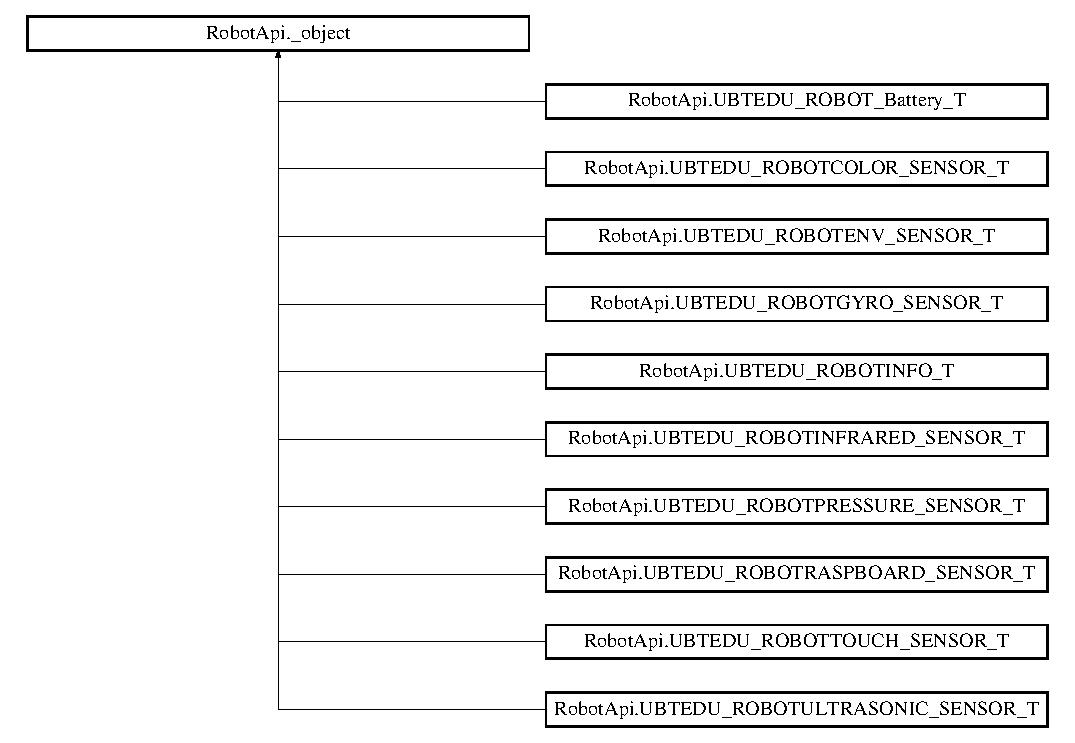
\includegraphics[height=9.535604cm]{classRobotApi_1_1__object}
\end{center}
\end{figure}


The documentation for this class was generated from the following file\+:\begin{DoxyCompactItemize}
\item 
Robot\+Api.\+py\end{DoxyCompactItemize}

\hypertarget{struct__RobotBatteryInfo}{\section{\+\_\+\+Robot\+Battery\+Info Struct Reference}
\label{struct__RobotBatteryInfo}\index{\+\_\+\+Robot\+Battery\+Info@{\+\_\+\+Robot\+Battery\+Info}}
}


Battery data.  




{\ttfamily \#include $<$Robot\+Api.\+h$>$}

\subsection*{Public Attributes}
\begin{DoxyCompactItemize}
\item 
int \hyperlink{struct__RobotBatteryInfo_a32d251261c450710c7fab260507e4383}{i\+Value} \mbox{[}3\mbox{]}
\end{DoxyCompactItemize}


\subsection{Detailed Description}
Battery data. 

\subsection{Member Data Documentation}
\hypertarget{struct__RobotBatteryInfo_a32d251261c450710c7fab260507e4383}{\index{\+\_\+\+Robot\+Battery\+Info@{\+\_\+\+Robot\+Battery\+Info}!i\+Value@{i\+Value}}
\index{i\+Value@{i\+Value}!\+\_\+\+Robot\+Battery\+Info@{\+\_\+\+Robot\+Battery\+Info}}
\subsubsection[{i\+Value}]{\setlength{\rightskip}{0pt plus 5cm}int \+\_\+\+Robot\+Battery\+Info\+::i\+Value\mbox{[}3\mbox{]}}}\label{struct__RobotBatteryInfo_a32d251261c450710c7fab260507e4383}
\mbox{[}0\mbox{]}\+: temperature, \mbox{[}1\mbox{]}\+: humidity, \mbox{[}2\mbox{]}\+: pressure 

The documentation for this struct was generated from the following file\+:\begin{DoxyCompactItemize}
\item 
\hyperlink{RobotApi_8h}{Robot\+Api.\+h}\end{DoxyCompactItemize}

\hypertarget{struct__RobotColorSensor}{\section{\+\_\+\+Robot\+Color\+Sensor Struct Reference}
\label{struct__RobotColorSensor}\index{\+\_\+\+Robot\+Color\+Sensor@{\+\_\+\+Robot\+Color\+Sensor}}
}


Color sensor data.  




{\ttfamily \#include $<$Robot\+Api.\+h$>$}

\subsection*{Public Attributes}
\begin{DoxyCompactItemize}
\item 
int \hyperlink{struct__RobotColorSensor_a38b270be1ee87849b7469d100e335314}{i\+Red\+Value}
\item 
int \hyperlink{struct__RobotColorSensor_acfeb66d972f8c3ab2a5982fd4aa3f630}{i\+Green\+Value}
\item 
int \hyperlink{struct__RobotColorSensor_ad5c72e4e33a2447d6514d1d5a13dc036}{i\+Blue\+Value}
\item 
int \hyperlink{struct__RobotColorSensor_afc18a2ae43409d1b74340f6f9d9fb677}{i\+Clear\+Value}
\end{DoxyCompactItemize}


\subsection{Detailed Description}
Color sensor data. 

\subsection{Member Data Documentation}
\hypertarget{struct__RobotColorSensor_ad5c72e4e33a2447d6514d1d5a13dc036}{\index{\+\_\+\+Robot\+Color\+Sensor@{\+\_\+\+Robot\+Color\+Sensor}!i\+Blue\+Value@{i\+Blue\+Value}}
\index{i\+Blue\+Value@{i\+Blue\+Value}!\+\_\+\+Robot\+Color\+Sensor@{\+\_\+\+Robot\+Color\+Sensor}}
\subsubsection[{i\+Blue\+Value}]{\setlength{\rightskip}{0pt plus 5cm}int \+\_\+\+Robot\+Color\+Sensor\+::i\+Blue\+Value}}\label{struct__RobotColorSensor_ad5c72e4e33a2447d6514d1d5a13dc036}
The Bluevalue of color sensor \hypertarget{struct__RobotColorSensor_afc18a2ae43409d1b74340f6f9d9fb677}{\index{\+\_\+\+Robot\+Color\+Sensor@{\+\_\+\+Robot\+Color\+Sensor}!i\+Clear\+Value@{i\+Clear\+Value}}
\index{i\+Clear\+Value@{i\+Clear\+Value}!\+\_\+\+Robot\+Color\+Sensor@{\+\_\+\+Robot\+Color\+Sensor}}
\subsubsection[{i\+Clear\+Value}]{\setlength{\rightskip}{0pt plus 5cm}int \+\_\+\+Robot\+Color\+Sensor\+::i\+Clear\+Value}}\label{struct__RobotColorSensor_afc18a2ae43409d1b74340f6f9d9fb677}
The Clear value of color sensor \hypertarget{struct__RobotColorSensor_acfeb66d972f8c3ab2a5982fd4aa3f630}{\index{\+\_\+\+Robot\+Color\+Sensor@{\+\_\+\+Robot\+Color\+Sensor}!i\+Green\+Value@{i\+Green\+Value}}
\index{i\+Green\+Value@{i\+Green\+Value}!\+\_\+\+Robot\+Color\+Sensor@{\+\_\+\+Robot\+Color\+Sensor}}
\subsubsection[{i\+Green\+Value}]{\setlength{\rightskip}{0pt plus 5cm}int \+\_\+\+Robot\+Color\+Sensor\+::i\+Green\+Value}}\label{struct__RobotColorSensor_acfeb66d972f8c3ab2a5982fd4aa3f630}
The Green value of color sensor \hypertarget{struct__RobotColorSensor_a38b270be1ee87849b7469d100e335314}{\index{\+\_\+\+Robot\+Color\+Sensor@{\+\_\+\+Robot\+Color\+Sensor}!i\+Red\+Value@{i\+Red\+Value}}
\index{i\+Red\+Value@{i\+Red\+Value}!\+\_\+\+Robot\+Color\+Sensor@{\+\_\+\+Robot\+Color\+Sensor}}
\subsubsection[{i\+Red\+Value}]{\setlength{\rightskip}{0pt plus 5cm}int \+\_\+\+Robot\+Color\+Sensor\+::i\+Red\+Value}}\label{struct__RobotColorSensor_a38b270be1ee87849b7469d100e335314}
The red value of color sensor 

The documentation for this struct was generated from the following file\+:\begin{DoxyCompactItemize}
\item 
\hyperlink{RobotApi_8h}{Robot\+Api.\+h}\end{DoxyCompactItemize}

\hypertarget{struct__RobotEnvSensor}{\section{\+\_\+\+Robot\+Env\+Sensor Struct Reference}
\label{struct__RobotEnvSensor}\index{\+\_\+\+Robot\+Env\+Sensor@{\+\_\+\+Robot\+Env\+Sensor}}
}


Environment sensor data.  




{\ttfamily \#include $<$Robot\+Api.\+h$>$}

\subsection*{Public Attributes}
\begin{DoxyCompactItemize}
\item 
int \hyperlink{struct__RobotEnvSensor_a43ada67fc341dfdadbad4b3c287cf3f4}{i\+Value} \mbox{[}3\mbox{]}
\end{DoxyCompactItemize}


\subsection{Detailed Description}
Environment sensor data. 

\subsection{Member Data Documentation}
\hypertarget{struct__RobotEnvSensor_a43ada67fc341dfdadbad4b3c287cf3f4}{\index{\+\_\+\+Robot\+Env\+Sensor@{\+\_\+\+Robot\+Env\+Sensor}!i\+Value@{i\+Value}}
\index{i\+Value@{i\+Value}!\+\_\+\+Robot\+Env\+Sensor@{\+\_\+\+Robot\+Env\+Sensor}}
\subsubsection[{i\+Value}]{\setlength{\rightskip}{0pt plus 5cm}int \+\_\+\+Robot\+Env\+Sensor\+::i\+Value\mbox{[}3\mbox{]}}}\label{struct__RobotEnvSensor_a43ada67fc341dfdadbad4b3c287cf3f4}
\mbox{[}0\mbox{]}\+: temperature, \mbox{[}1\mbox{]}\+: humidity, \mbox{[}2\mbox{]}\+: pressure 

The documentation for this struct was generated from the following file\+:\begin{DoxyCompactItemize}
\item 
\hyperlink{RobotApi_8h}{Robot\+Api.\+h}\end{DoxyCompactItemize}

\hypertarget{struct__RobotGyroSensor}{\section{\+\_\+\+Robot\+Gyro\+Sensor Struct Reference}
\label{struct__RobotGyroSensor}\index{\+\_\+\+Robot\+Gyro\+Sensor@{\+\_\+\+Robot\+Gyro\+Sensor}}
}


Gyro sensor data.  




{\ttfamily \#include $<$Robot\+Api.\+h$>$}

\subsection*{Public Attributes}
\begin{DoxyCompactItemize}
\item 
double \hyperlink{struct__RobotGyroSensor_a0dbe9c8f5dd0cd4b931565d1db0e0f6e}{d\+Value} \mbox{[}4 $\ast$3\mbox{]}
\end{DoxyCompactItemize}


\subsection{Detailed Description}
Gyro sensor data. 

\subsection{Member Data Documentation}
\hypertarget{struct__RobotGyroSensor_a0dbe9c8f5dd0cd4b931565d1db0e0f6e}{\index{\+\_\+\+Robot\+Gyro\+Sensor@{\+\_\+\+Robot\+Gyro\+Sensor}!d\+Value@{d\+Value}}
\index{d\+Value@{d\+Value}!\+\_\+\+Robot\+Gyro\+Sensor@{\+\_\+\+Robot\+Gyro\+Sensor}}
\subsubsection[{d\+Value}]{\setlength{\rightskip}{0pt plus 5cm}double \+\_\+\+Robot\+Gyro\+Sensor\+::d\+Value\mbox{[}4 $\ast$3\mbox{]}}}\label{struct__RobotGyroSensor_a0dbe9c8f5dd0cd4b931565d1db0e0f6e}
Gyro x,y,z accelerate x,y,z compass x,y,z euler x,y,z 

The documentation for this struct was generated from the following file\+:\begin{DoxyCompactItemize}
\item 
\hyperlink{RobotApi_8h}{Robot\+Api.\+h}\end{DoxyCompactItemize}

\hypertarget{struct__RobotInfo}{\section{\+\_\+\+Robot\+Info Struct Reference}
\label{struct__RobotInfo}\index{\+\_\+\+Robot\+Info@{\+\_\+\+Robot\+Info}}
}


Robot infomation.  




{\ttfamily \#include $<$Robot\+Api.\+h$>$}

\subsection*{Public Attributes}
\begin{DoxyCompactItemize}
\item 
\hypertarget{struct__RobotInfo_a0dc600adfbf72150e776f100d6ec80ad}{char {\bfseries ac\+Name} \mbox{[}U\+B\+T\+E\+D\+U\+\_\+\+R\+O\+B\+O\+T\+\_\+\+N\+A\+M\+E\+\_\+\+L\+E\+N\mbox{]}}\label{struct__RobotInfo_a0dc600adfbf72150e776f100d6ec80ad}

\item 
\hypertarget{struct__RobotInfo_aca220e4bd42b444cc5f105c4ceaf2760}{char {\bfseries ac\+I\+P\+Addr} \mbox{[}U\+B\+T\+E\+D\+U\+\_\+\+R\+O\+B\+O\+T\+\_\+\+I\+P\+\_\+\+A\+D\+D\+R\+\_\+\+L\+E\+N\mbox{]}}\label{struct__RobotInfo_aca220e4bd42b444cc5f105c4ceaf2760}

\end{DoxyCompactItemize}


\subsection{Detailed Description}
Robot infomation. 

The documentation for this struct was generated from the following file\+:\begin{DoxyCompactItemize}
\item 
\hyperlink{RobotApi_8h}{Robot\+Api.\+h}\end{DoxyCompactItemize}

\hypertarget{struct__RobotInfraredSensor}{\section{\+\_\+\+Robot\+Infrared\+Sensor Struct Reference}
\label{struct__RobotInfraredSensor}\index{\+\_\+\+Robot\+Infrared\+Sensor@{\+\_\+\+Robot\+Infrared\+Sensor}}
}


Infrared sensor data.  




{\ttfamily \#include $<$Robot\+Api.\+h$>$}

\subsection*{Public Attributes}
\begin{DoxyCompactItemize}
\item 
int \hyperlink{struct__RobotInfraredSensor_adc590c79e4a6f32cc761bb95f6235986}{i\+Value}
\end{DoxyCompactItemize}


\subsection{Detailed Description}
Infrared sensor data. 

\subsection{Member Data Documentation}
\hypertarget{struct__RobotInfraredSensor_adc590c79e4a6f32cc761bb95f6235986}{\index{\+\_\+\+Robot\+Infrared\+Sensor@{\+\_\+\+Robot\+Infrared\+Sensor}!i\+Value@{i\+Value}}
\index{i\+Value@{i\+Value}!\+\_\+\+Robot\+Infrared\+Sensor@{\+\_\+\+Robot\+Infrared\+Sensor}}
\subsubsection[{i\+Value}]{\setlength{\rightskip}{0pt plus 5cm}int \+\_\+\+Robot\+Infrared\+Sensor\+::i\+Value}}\label{struct__RobotInfraredSensor_adc590c79e4a6f32cc761bb95f6235986}
The distance via infrared sensor 

The documentation for this struct was generated from the following file\+:\begin{DoxyCompactItemize}
\item 
\hyperlink{RobotApi_8h}{Robot\+Api.\+h}\end{DoxyCompactItemize}

\hypertarget{struct__RobotPressureSensor}{\section{\+\_\+\+Robot\+Pressure\+Sensor Struct Reference}
\label{struct__RobotPressureSensor}\index{\+\_\+\+Robot\+Pressure\+Sensor@{\+\_\+\+Robot\+Pressure\+Sensor}}
}


Pressure sensor data.  




{\ttfamily \#include $<$Robot\+Api.\+h$>$}

\subsection*{Public Attributes}
\begin{DoxyCompactItemize}
\item 
int \hyperlink{struct__RobotPressureSensor_aa8cde267cdbc78067d0589e15e9fb15d}{i\+Value}
\end{DoxyCompactItemize}


\subsection{Detailed Description}
Pressure sensor data. 

\subsection{Member Data Documentation}
\hypertarget{struct__RobotPressureSensor_aa8cde267cdbc78067d0589e15e9fb15d}{\index{\+\_\+\+Robot\+Pressure\+Sensor@{\+\_\+\+Robot\+Pressure\+Sensor}!i\+Value@{i\+Value}}
\index{i\+Value@{i\+Value}!\+\_\+\+Robot\+Pressure\+Sensor@{\+\_\+\+Robot\+Pressure\+Sensor}}
\subsubsection[{i\+Value}]{\setlength{\rightskip}{0pt plus 5cm}int \+\_\+\+Robot\+Pressure\+Sensor\+::i\+Value}}\label{struct__RobotPressureSensor_aa8cde267cdbc78067d0589e15e9fb15d}
The Pressure via Pressure sensor 

The documentation for this struct was generated from the following file\+:\begin{DoxyCompactItemize}
\item 
\hyperlink{RobotApi_8h}{Robot\+Api.\+h}\end{DoxyCompactItemize}

\hypertarget{struct__RobotRaspPiBoardSensor}{\section{\+\_\+\+Robot\+Rasp\+Pi\+Board\+Sensor Struct Reference}
\label{struct__RobotRaspPiBoardSensor}\index{\+\_\+\+Robot\+Rasp\+Pi\+Board\+Sensor@{\+\_\+\+Robot\+Rasp\+Pi\+Board\+Sensor}}
}


Raspberry Pi board P\+C\+B data.  




{\ttfamily \#include $<$Robot\+Api.\+h$>$}

\subsection*{Public Attributes}
\begin{DoxyCompactItemize}
\item 
int \hyperlink{struct__RobotRaspPiBoardSensor_a6121402932f93d71f7b1140d087079cf}{i\+Value}
\end{DoxyCompactItemize}


\subsection{Detailed Description}
Raspberry Pi board P\+C\+B data. 

\subsection{Member Data Documentation}
\hypertarget{struct__RobotRaspPiBoardSensor_a6121402932f93d71f7b1140d087079cf}{\index{\+\_\+\+Robot\+Rasp\+Pi\+Board\+Sensor@{\+\_\+\+Robot\+Rasp\+Pi\+Board\+Sensor}!i\+Value@{i\+Value}}
\index{i\+Value@{i\+Value}!\+\_\+\+Robot\+Rasp\+Pi\+Board\+Sensor@{\+\_\+\+Robot\+Rasp\+Pi\+Board\+Sensor}}
\subsubsection[{i\+Value}]{\setlength{\rightskip}{0pt plus 5cm}int \+\_\+\+Robot\+Rasp\+Pi\+Board\+Sensor\+::i\+Value}}\label{struct__RobotRaspPiBoardSensor_a6121402932f93d71f7b1140d087079cf}
Board temperature 

The documentation for this struct was generated from the following file\+:\begin{DoxyCompactItemize}
\item 
\hyperlink{RobotApi_8h}{Robot\+Api.\+h}\end{DoxyCompactItemize}

\hypertarget{struct__RobotTouchSensor}{\section{\+\_\+\+Robot\+Touch\+Sensor Struct Reference}
\label{struct__RobotTouchSensor}\index{\+\_\+\+Robot\+Touch\+Sensor@{\+\_\+\+Robot\+Touch\+Sensor}}
}


Touch sensor data.  




{\ttfamily \#include $<$Robot\+Api.\+h$>$}

\subsection*{Public Attributes}
\begin{DoxyCompactItemize}
\item 
int \hyperlink{struct__RobotTouchSensor_add5e6cd8bce6fb09abbfd6c3f09a3faa}{i\+Value}
\end{DoxyCompactItemize}


\subsection{Detailed Description}
Touch sensor data. 

\subsection{Member Data Documentation}
\hypertarget{struct__RobotTouchSensor_add5e6cd8bce6fb09abbfd6c3f09a3faa}{\index{\+\_\+\+Robot\+Touch\+Sensor@{\+\_\+\+Robot\+Touch\+Sensor}!i\+Value@{i\+Value}}
\index{i\+Value@{i\+Value}!\+\_\+\+Robot\+Touch\+Sensor@{\+\_\+\+Robot\+Touch\+Sensor}}
\subsubsection[{i\+Value}]{\setlength{\rightskip}{0pt plus 5cm}int \+\_\+\+Robot\+Touch\+Sensor\+::i\+Value}}\label{struct__RobotTouchSensor_add5e6cd8bce6fb09abbfd6c3f09a3faa}
The Touch sensor 

The documentation for this struct was generated from the following file\+:\begin{DoxyCompactItemize}
\item 
\hyperlink{RobotApi_8h}{Robot\+Api.\+h}\end{DoxyCompactItemize}

\hypertarget{struct__RobotUltrasonicSensor}{\section{\+\_\+\+Robot\+Ultrasonic\+Sensor Struct Reference}
\label{struct__RobotUltrasonicSensor}\index{\+\_\+\+Robot\+Ultrasonic\+Sensor@{\+\_\+\+Robot\+Ultrasonic\+Sensor}}
}


Ultrasonic sensor data.  




{\ttfamily \#include $<$Robot\+Api.\+h$>$}

\subsection*{Public Attributes}
\begin{DoxyCompactItemize}
\item 
int \hyperlink{struct__RobotUltrasonicSensor_a5ca5e4487dcbe1a83820e06ddcd9c047}{i\+Value}
\end{DoxyCompactItemize}


\subsection{Detailed Description}
Ultrasonic sensor data. 

\subsection{Member Data Documentation}
\hypertarget{struct__RobotUltrasonicSensor_a5ca5e4487dcbe1a83820e06ddcd9c047}{\index{\+\_\+\+Robot\+Ultrasonic\+Sensor@{\+\_\+\+Robot\+Ultrasonic\+Sensor}!i\+Value@{i\+Value}}
\index{i\+Value@{i\+Value}!\+\_\+\+Robot\+Ultrasonic\+Sensor@{\+\_\+\+Robot\+Ultrasonic\+Sensor}}
\subsubsection[{i\+Value}]{\setlength{\rightskip}{0pt plus 5cm}int \+\_\+\+Robot\+Ultrasonic\+Sensor\+::i\+Value}}\label{struct__RobotUltrasonicSensor_a5ca5e4487dcbe1a83820e06ddcd9c047}
The distance via ultrasonic sensor 

The documentation for this struct was generated from the following file\+:\begin{DoxyCompactItemize}
\item 
\hyperlink{RobotApi_8h}{Robot\+Api.\+h}\end{DoxyCompactItemize}

\hypertarget{classRobotApi_1_1UBTEDU__ROBOT__Battery__T}{\section{Robot\+Api.\+U\+B\+T\+E\+D\+U\+\_\+\+R\+O\+B\+O\+T\+\_\+\+Battery\+\_\+\+T Class Reference}
\label{classRobotApi_1_1UBTEDU__ROBOT__Battery__T}\index{Robot\+Api.\+U\+B\+T\+E\+D\+U\+\_\+\+R\+O\+B\+O\+T\+\_\+\+Battery\+\_\+\+T@{Robot\+Api.\+U\+B\+T\+E\+D\+U\+\_\+\+R\+O\+B\+O\+T\+\_\+\+Battery\+\_\+\+T}}
}
Inheritance diagram for Robot\+Api.\+U\+B\+T\+E\+D\+U\+\_\+\+R\+O\+B\+O\+T\+\_\+\+Battery\+\_\+\+T\+:\begin{figure}[H]
\begin{center}
\leavevmode
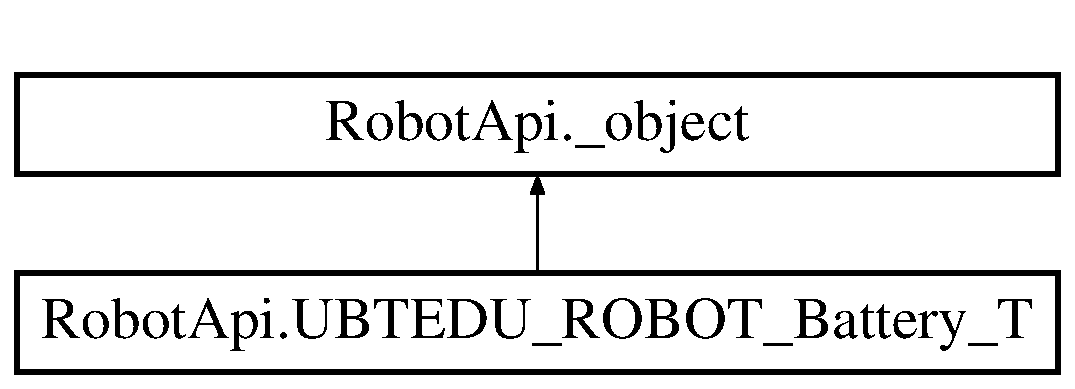
\includegraphics[height=2.000000cm]{classRobotApi_1_1UBTEDU__ROBOT__Battery__T}
\end{center}
\end{figure}
\subsection*{Public Member Functions}
\begin{DoxyCompactItemize}
\item 
\hypertarget{classRobotApi_1_1UBTEDU__ROBOT__Battery__T_a6696b4924b64f4d15dcc4d080af4e63c}{def {\bfseries \+\_\+\+\_\+init\+\_\+\+\_\+}}\label{classRobotApi_1_1UBTEDU__ROBOT__Battery__T_a6696b4924b64f4d15dcc4d080af4e63c}

\end{DoxyCompactItemize}
\subsection*{Public Attributes}
\begin{DoxyCompactItemize}
\item 
\hypertarget{classRobotApi_1_1UBTEDU__ROBOT__Battery__T_a79ac9be20b2d864afb186cd79d6e9ad6}{{\bfseries this}}\label{classRobotApi_1_1UBTEDU__ROBOT__Battery__T_a79ac9be20b2d864afb186cd79d6e9ad6}

\end{DoxyCompactItemize}


The documentation for this class was generated from the following file\+:\begin{DoxyCompactItemize}
\item 
Robot\+Api.\+py\end{DoxyCompactItemize}

\hypertarget{classRobotApi_1_1UBTEDU__ROBOTCOLOR__SENSOR__T}{\section{Robot\+Api.\+U\+B\+T\+E\+D\+U\+\_\+\+R\+O\+B\+O\+T\+C\+O\+L\+O\+R\+\_\+\+S\+E\+N\+S\+O\+R\+\_\+\+T Class Reference}
\label{classRobotApi_1_1UBTEDU__ROBOTCOLOR__SENSOR__T}\index{Robot\+Api.\+U\+B\+T\+E\+D\+U\+\_\+\+R\+O\+B\+O\+T\+C\+O\+L\+O\+R\+\_\+\+S\+E\+N\+S\+O\+R\+\_\+\+T@{Robot\+Api.\+U\+B\+T\+E\+D\+U\+\_\+\+R\+O\+B\+O\+T\+C\+O\+L\+O\+R\+\_\+\+S\+E\+N\+S\+O\+R\+\_\+\+T}}
}
Inheritance diagram for Robot\+Api.\+U\+B\+T\+E\+D\+U\+\_\+\+R\+O\+B\+O\+T\+C\+O\+L\+O\+R\+\_\+\+S\+E\+N\+S\+O\+R\+\_\+\+T\+:\begin{figure}[H]
\begin{center}
\leavevmode
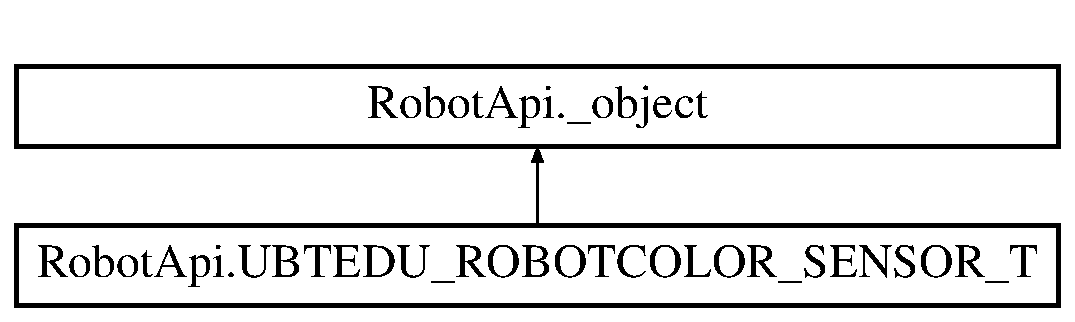
\includegraphics[height=2.000000cm]{classRobotApi_1_1UBTEDU__ROBOTCOLOR__SENSOR__T}
\end{center}
\end{figure}
\subsection*{Public Member Functions}
\begin{DoxyCompactItemize}
\item 
\hypertarget{classRobotApi_1_1UBTEDU__ROBOTCOLOR__SENSOR__T_af3082be93049be25f5cd05910cd990f3}{def {\bfseries \+\_\+\+\_\+init\+\_\+\+\_\+}}\label{classRobotApi_1_1UBTEDU__ROBOTCOLOR__SENSOR__T_af3082be93049be25f5cd05910cd990f3}

\end{DoxyCompactItemize}
\subsection*{Public Attributes}
\begin{DoxyCompactItemize}
\item 
\hypertarget{classRobotApi_1_1UBTEDU__ROBOTCOLOR__SENSOR__T_a12fa414a9c369471637a6afaed937d87}{{\bfseries this}}\label{classRobotApi_1_1UBTEDU__ROBOTCOLOR__SENSOR__T_a12fa414a9c369471637a6afaed937d87}

\end{DoxyCompactItemize}


The documentation for this class was generated from the following file\+:\begin{DoxyCompactItemize}
\item 
Robot\+Api.\+py\end{DoxyCompactItemize}

\hypertarget{classRobotApi_1_1UBTEDU__ROBOTENV__SENSOR__T}{\section{Robot\+Api.\+U\+B\+T\+E\+D\+U\+\_\+\+R\+O\+B\+O\+T\+E\+N\+V\+\_\+\+S\+E\+N\+S\+O\+R\+\_\+\+T Class Reference}
\label{classRobotApi_1_1UBTEDU__ROBOTENV__SENSOR__T}\index{Robot\+Api.\+U\+B\+T\+E\+D\+U\+\_\+\+R\+O\+B\+O\+T\+E\+N\+V\+\_\+\+S\+E\+N\+S\+O\+R\+\_\+\+T@{Robot\+Api.\+U\+B\+T\+E\+D\+U\+\_\+\+R\+O\+B\+O\+T\+E\+N\+V\+\_\+\+S\+E\+N\+S\+O\+R\+\_\+\+T}}
}
Inheritance diagram for Robot\+Api.\+U\+B\+T\+E\+D\+U\+\_\+\+R\+O\+B\+O\+T\+E\+N\+V\+\_\+\+S\+E\+N\+S\+O\+R\+\_\+\+T\+:\begin{figure}[H]
\begin{center}
\leavevmode
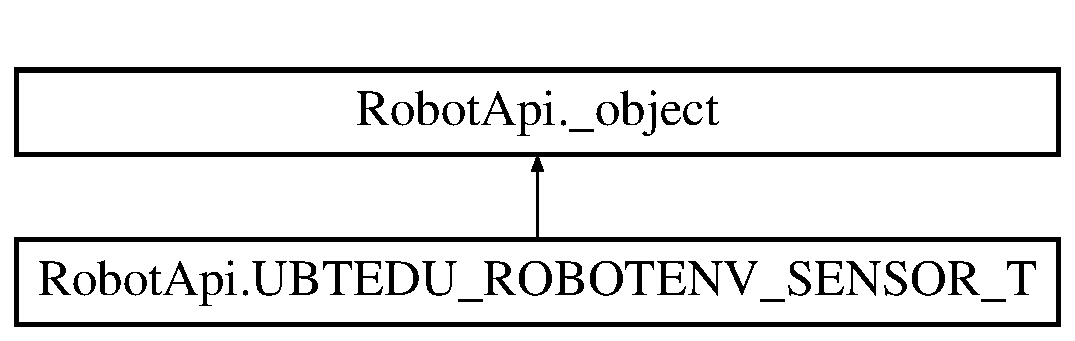
\includegraphics[height=2.000000cm]{classRobotApi_1_1UBTEDU__ROBOTENV__SENSOR__T}
\end{center}
\end{figure}
\subsection*{Public Member Functions}
\begin{DoxyCompactItemize}
\item 
\hypertarget{classRobotApi_1_1UBTEDU__ROBOTENV__SENSOR__T_a2fe446e45a2ded461a9c8a7ca48d88fe}{def {\bfseries \+\_\+\+\_\+init\+\_\+\+\_\+}}\label{classRobotApi_1_1UBTEDU__ROBOTENV__SENSOR__T_a2fe446e45a2ded461a9c8a7ca48d88fe}

\end{DoxyCompactItemize}
\subsection*{Public Attributes}
\begin{DoxyCompactItemize}
\item 
\hypertarget{classRobotApi_1_1UBTEDU__ROBOTENV__SENSOR__T_a15d4edcdaea27efa92b9b5ae31992a41}{{\bfseries this}}\label{classRobotApi_1_1UBTEDU__ROBOTENV__SENSOR__T_a15d4edcdaea27efa92b9b5ae31992a41}

\end{DoxyCompactItemize}


The documentation for this class was generated from the following file\+:\begin{DoxyCompactItemize}
\item 
Robot\+Api.\+py\end{DoxyCompactItemize}

\hypertarget{classRobotApi_1_1UBTEDU__ROBOTGYRO__SENSOR__T}{\section{Robot\+Api.\+U\+B\+T\+E\+D\+U\+\_\+\+R\+O\+B\+O\+T\+G\+Y\+R\+O\+\_\+\+S\+E\+N\+S\+O\+R\+\_\+\+T Class Reference}
\label{classRobotApi_1_1UBTEDU__ROBOTGYRO__SENSOR__T}\index{Robot\+Api.\+U\+B\+T\+E\+D\+U\+\_\+\+R\+O\+B\+O\+T\+G\+Y\+R\+O\+\_\+\+S\+E\+N\+S\+O\+R\+\_\+\+T@{Robot\+Api.\+U\+B\+T\+E\+D\+U\+\_\+\+R\+O\+B\+O\+T\+G\+Y\+R\+O\+\_\+\+S\+E\+N\+S\+O\+R\+\_\+\+T}}
}
Inheritance diagram for Robot\+Api.\+U\+B\+T\+E\+D\+U\+\_\+\+R\+O\+B\+O\+T\+G\+Y\+R\+O\+\_\+\+S\+E\+N\+S\+O\+R\+\_\+\+T\+:\begin{figure}[H]
\begin{center}
\leavevmode
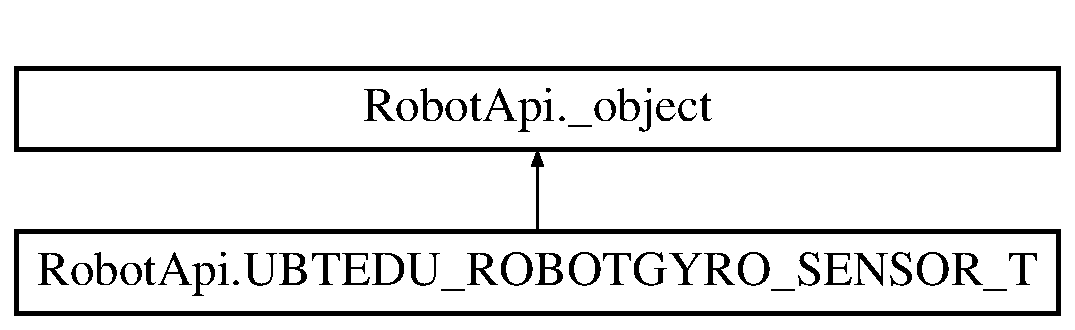
\includegraphics[height=2.000000cm]{classRobotApi_1_1UBTEDU__ROBOTGYRO__SENSOR__T}
\end{center}
\end{figure}
\subsection*{Public Member Functions}
\begin{DoxyCompactItemize}
\item 
\hypertarget{classRobotApi_1_1UBTEDU__ROBOTGYRO__SENSOR__T_a8e59f7437428060495a2c7dbe6eb6d01}{def {\bfseries \+\_\+\+\_\+init\+\_\+\+\_\+}}\label{classRobotApi_1_1UBTEDU__ROBOTGYRO__SENSOR__T_a8e59f7437428060495a2c7dbe6eb6d01}

\end{DoxyCompactItemize}
\subsection*{Public Attributes}
\begin{DoxyCompactItemize}
\item 
\hypertarget{classRobotApi_1_1UBTEDU__ROBOTGYRO__SENSOR__T_a1f5c9b1c0554aba851b7fc131eacbb25}{{\bfseries this}}\label{classRobotApi_1_1UBTEDU__ROBOTGYRO__SENSOR__T_a1f5c9b1c0554aba851b7fc131eacbb25}

\end{DoxyCompactItemize}


The documentation for this class was generated from the following file\+:\begin{DoxyCompactItemize}
\item 
Robot\+Api.\+py\end{DoxyCompactItemize}

\hypertarget{classRobotApi_1_1UBTEDU__ROBOTINFO__T}{\section{Robot\+Api.\+U\+B\+T\+E\+D\+U\+\_\+\+R\+O\+B\+O\+T\+I\+N\+F\+O\+\_\+\+T Class Reference}
\label{classRobotApi_1_1UBTEDU__ROBOTINFO__T}\index{Robot\+Api.\+U\+B\+T\+E\+D\+U\+\_\+\+R\+O\+B\+O\+T\+I\+N\+F\+O\+\_\+\+T@{Robot\+Api.\+U\+B\+T\+E\+D\+U\+\_\+\+R\+O\+B\+O\+T\+I\+N\+F\+O\+\_\+\+T}}
}
Inheritance diagram for Robot\+Api.\+U\+B\+T\+E\+D\+U\+\_\+\+R\+O\+B\+O\+T\+I\+N\+F\+O\+\_\+\+T\+:\begin{figure}[H]
\begin{center}
\leavevmode
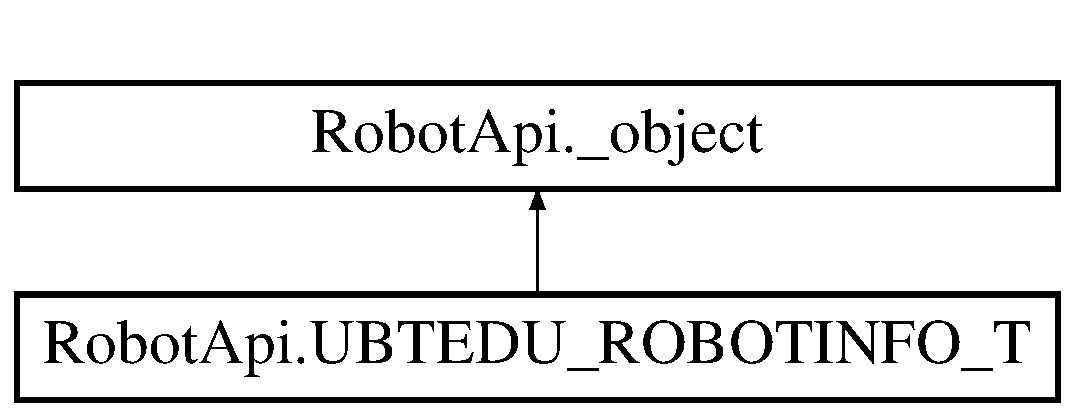
\includegraphics[height=2.000000cm]{classRobotApi_1_1UBTEDU__ROBOTINFO__T}
\end{center}
\end{figure}
\subsection*{Public Member Functions}
\begin{DoxyCompactItemize}
\item 
\hypertarget{classRobotApi_1_1UBTEDU__ROBOTINFO__T_a4a1c2f5b9e2914a135f345e11389b38a}{def {\bfseries \+\_\+\+\_\+init\+\_\+\+\_\+}}\label{classRobotApi_1_1UBTEDU__ROBOTINFO__T_a4a1c2f5b9e2914a135f345e11389b38a}

\end{DoxyCompactItemize}
\subsection*{Public Attributes}
\begin{DoxyCompactItemize}
\item 
\hypertarget{classRobotApi_1_1UBTEDU__ROBOTINFO__T_ab9befe76e1e0980a75d9555bd7b594da}{{\bfseries this}}\label{classRobotApi_1_1UBTEDU__ROBOTINFO__T_ab9befe76e1e0980a75d9555bd7b594da}

\end{DoxyCompactItemize}


The documentation for this class was generated from the following file\+:\begin{DoxyCompactItemize}
\item 
Robot\+Api.\+py\end{DoxyCompactItemize}

\hypertarget{classRobotApi_1_1UBTEDU__ROBOTINFRARED__SENSOR__T}{\section{Robot\+Api.\+U\+B\+T\+E\+D\+U\+\_\+\+R\+O\+B\+O\+T\+I\+N\+F\+R\+A\+R\+E\+D\+\_\+\+S\+E\+N\+S\+O\+R\+\_\+\+T Class Reference}
\label{classRobotApi_1_1UBTEDU__ROBOTINFRARED__SENSOR__T}\index{Robot\+Api.\+U\+B\+T\+E\+D\+U\+\_\+\+R\+O\+B\+O\+T\+I\+N\+F\+R\+A\+R\+E\+D\+\_\+\+S\+E\+N\+S\+O\+R\+\_\+\+T@{Robot\+Api.\+U\+B\+T\+E\+D\+U\+\_\+\+R\+O\+B\+O\+T\+I\+N\+F\+R\+A\+R\+E\+D\+\_\+\+S\+E\+N\+S\+O\+R\+\_\+\+T}}
}
Inheritance diagram for Robot\+Api.\+U\+B\+T\+E\+D\+U\+\_\+\+R\+O\+B\+O\+T\+I\+N\+F\+R\+A\+R\+E\+D\+\_\+\+S\+E\+N\+S\+O\+R\+\_\+\+T\+:\begin{figure}[H]
\begin{center}
\leavevmode
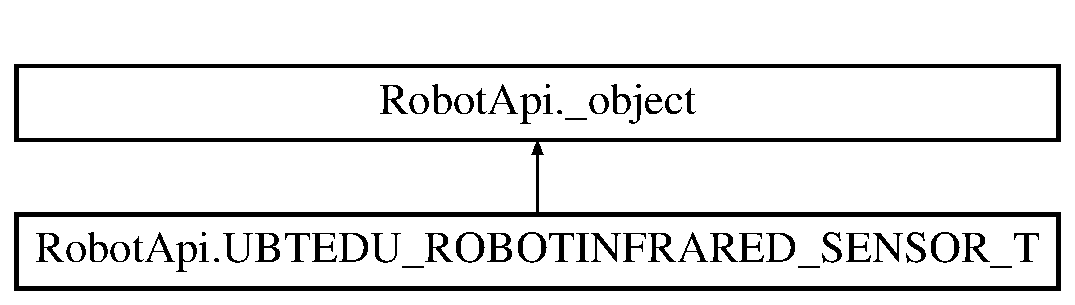
\includegraphics[height=2.000000cm]{classRobotApi_1_1UBTEDU__ROBOTINFRARED__SENSOR__T}
\end{center}
\end{figure}
\subsection*{Public Member Functions}
\begin{DoxyCompactItemize}
\item 
\hypertarget{classRobotApi_1_1UBTEDU__ROBOTINFRARED__SENSOR__T_a6fcdd37a48aa53d3507e440b8fd71fe1}{def {\bfseries \+\_\+\+\_\+init\+\_\+\+\_\+}}\label{classRobotApi_1_1UBTEDU__ROBOTINFRARED__SENSOR__T_a6fcdd37a48aa53d3507e440b8fd71fe1}

\end{DoxyCompactItemize}
\subsection*{Public Attributes}
\begin{DoxyCompactItemize}
\item 
\hypertarget{classRobotApi_1_1UBTEDU__ROBOTINFRARED__SENSOR__T_ab5817918c360ebdf3491c8316c48cead}{{\bfseries this}}\label{classRobotApi_1_1UBTEDU__ROBOTINFRARED__SENSOR__T_ab5817918c360ebdf3491c8316c48cead}

\end{DoxyCompactItemize}


The documentation for this class was generated from the following file\+:\begin{DoxyCompactItemize}
\item 
Robot\+Api.\+py\end{DoxyCompactItemize}

\hypertarget{classRobotApi_1_1UBTEDU__ROBOTPRESSURE__SENSOR__T}{\section{Robot\+Api.\+U\+B\+T\+E\+D\+U\+\_\+\+R\+O\+B\+O\+T\+P\+R\+E\+S\+S\+U\+R\+E\+\_\+\+S\+E\+N\+S\+O\+R\+\_\+\+T Class Reference}
\label{classRobotApi_1_1UBTEDU__ROBOTPRESSURE__SENSOR__T}\index{Robot\+Api.\+U\+B\+T\+E\+D\+U\+\_\+\+R\+O\+B\+O\+T\+P\+R\+E\+S\+S\+U\+R\+E\+\_\+\+S\+E\+N\+S\+O\+R\+\_\+\+T@{Robot\+Api.\+U\+B\+T\+E\+D\+U\+\_\+\+R\+O\+B\+O\+T\+P\+R\+E\+S\+S\+U\+R\+E\+\_\+\+S\+E\+N\+S\+O\+R\+\_\+\+T}}
}
Inheritance diagram for Robot\+Api.\+U\+B\+T\+E\+D\+U\+\_\+\+R\+O\+B\+O\+T\+P\+R\+E\+S\+S\+U\+R\+E\+\_\+\+S\+E\+N\+S\+O\+R\+\_\+\+T\+:\begin{figure}[H]
\begin{center}
\leavevmode
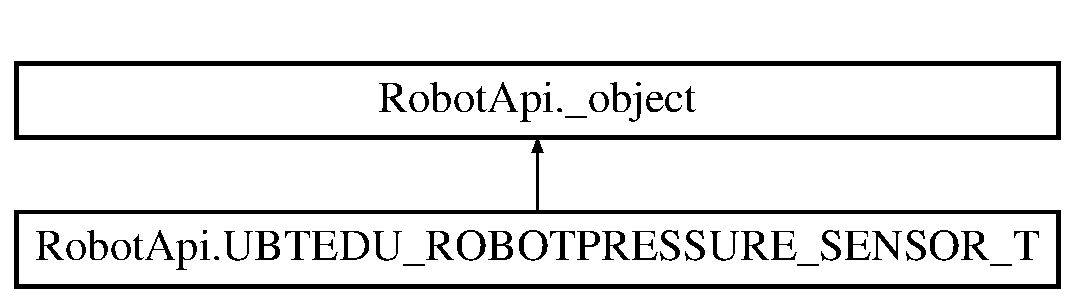
\includegraphics[height=2.000000cm]{classRobotApi_1_1UBTEDU__ROBOTPRESSURE__SENSOR__T}
\end{center}
\end{figure}
\subsection*{Public Member Functions}
\begin{DoxyCompactItemize}
\item 
\hypertarget{classRobotApi_1_1UBTEDU__ROBOTPRESSURE__SENSOR__T_a454f0b56ebd0309d9f0e418694e1443f}{def {\bfseries \+\_\+\+\_\+init\+\_\+\+\_\+}}\label{classRobotApi_1_1UBTEDU__ROBOTPRESSURE__SENSOR__T_a454f0b56ebd0309d9f0e418694e1443f}

\end{DoxyCompactItemize}
\subsection*{Public Attributes}
\begin{DoxyCompactItemize}
\item 
\hypertarget{classRobotApi_1_1UBTEDU__ROBOTPRESSURE__SENSOR__T_a3637350305a0ed076e9e5d0ff0506884}{{\bfseries this}}\label{classRobotApi_1_1UBTEDU__ROBOTPRESSURE__SENSOR__T_a3637350305a0ed076e9e5d0ff0506884}

\end{DoxyCompactItemize}


The documentation for this class was generated from the following file\+:\begin{DoxyCompactItemize}
\item 
Robot\+Api.\+py\end{DoxyCompactItemize}

\hypertarget{classRobotApi_1_1UBTEDU__ROBOTRASPBOARD__SENSOR__T}{\section{Robot\+Api.\+U\+B\+T\+E\+D\+U\+\_\+\+R\+O\+B\+O\+T\+R\+A\+S\+P\+B\+O\+A\+R\+D\+\_\+\+S\+E\+N\+S\+O\+R\+\_\+\+T Class Reference}
\label{classRobotApi_1_1UBTEDU__ROBOTRASPBOARD__SENSOR__T}\index{Robot\+Api.\+U\+B\+T\+E\+D\+U\+\_\+\+R\+O\+B\+O\+T\+R\+A\+S\+P\+B\+O\+A\+R\+D\+\_\+\+S\+E\+N\+S\+O\+R\+\_\+\+T@{Robot\+Api.\+U\+B\+T\+E\+D\+U\+\_\+\+R\+O\+B\+O\+T\+R\+A\+S\+P\+B\+O\+A\+R\+D\+\_\+\+S\+E\+N\+S\+O\+R\+\_\+\+T}}
}
Inheritance diagram for Robot\+Api.\+U\+B\+T\+E\+D\+U\+\_\+\+R\+O\+B\+O\+T\+R\+A\+S\+P\+B\+O\+A\+R\+D\+\_\+\+S\+E\+N\+S\+O\+R\+\_\+\+T\+:\begin{figure}[H]
\begin{center}
\leavevmode
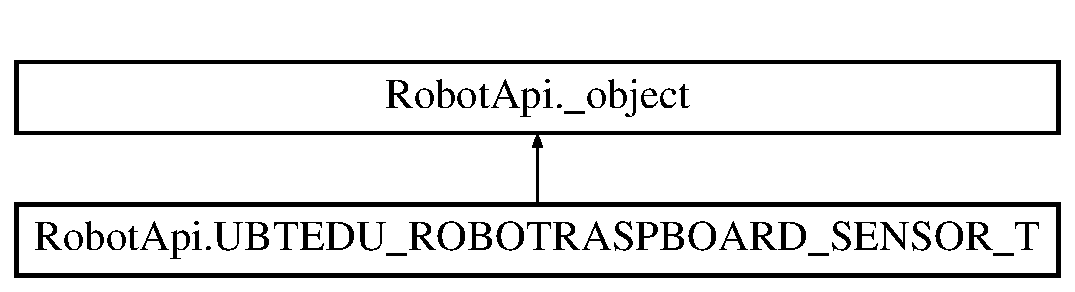
\includegraphics[height=2.000000cm]{classRobotApi_1_1UBTEDU__ROBOTRASPBOARD__SENSOR__T}
\end{center}
\end{figure}
\subsection*{Public Member Functions}
\begin{DoxyCompactItemize}
\item 
\hypertarget{classRobotApi_1_1UBTEDU__ROBOTRASPBOARD__SENSOR__T_a83d482f7d2ef8538211ca356d190ce92}{def {\bfseries \+\_\+\+\_\+init\+\_\+\+\_\+}}\label{classRobotApi_1_1UBTEDU__ROBOTRASPBOARD__SENSOR__T_a83d482f7d2ef8538211ca356d190ce92}

\end{DoxyCompactItemize}
\subsection*{Public Attributes}
\begin{DoxyCompactItemize}
\item 
\hypertarget{classRobotApi_1_1UBTEDU__ROBOTRASPBOARD__SENSOR__T_abee597ebf9d71c1e75580f10a452b662}{{\bfseries this}}\label{classRobotApi_1_1UBTEDU__ROBOTRASPBOARD__SENSOR__T_abee597ebf9d71c1e75580f10a452b662}

\end{DoxyCompactItemize}


The documentation for this class was generated from the following file\+:\begin{DoxyCompactItemize}
\item 
Robot\+Api.\+py\end{DoxyCompactItemize}

\hypertarget{classRobotApi_1_1UBTEDU__ROBOTTOUCH__SENSOR__T}{\section{Robot\+Api.\+U\+B\+T\+E\+D\+U\+\_\+\+R\+O\+B\+O\+T\+T\+O\+U\+C\+H\+\_\+\+S\+E\+N\+S\+O\+R\+\_\+\+T Class Reference}
\label{classRobotApi_1_1UBTEDU__ROBOTTOUCH__SENSOR__T}\index{Robot\+Api.\+U\+B\+T\+E\+D\+U\+\_\+\+R\+O\+B\+O\+T\+T\+O\+U\+C\+H\+\_\+\+S\+E\+N\+S\+O\+R\+\_\+\+T@{Robot\+Api.\+U\+B\+T\+E\+D\+U\+\_\+\+R\+O\+B\+O\+T\+T\+O\+U\+C\+H\+\_\+\+S\+E\+N\+S\+O\+R\+\_\+\+T}}
}
Inheritance diagram for Robot\+Api.\+U\+B\+T\+E\+D\+U\+\_\+\+R\+O\+B\+O\+T\+T\+O\+U\+C\+H\+\_\+\+S\+E\+N\+S\+O\+R\+\_\+\+T\+:\begin{figure}[H]
\begin{center}
\leavevmode
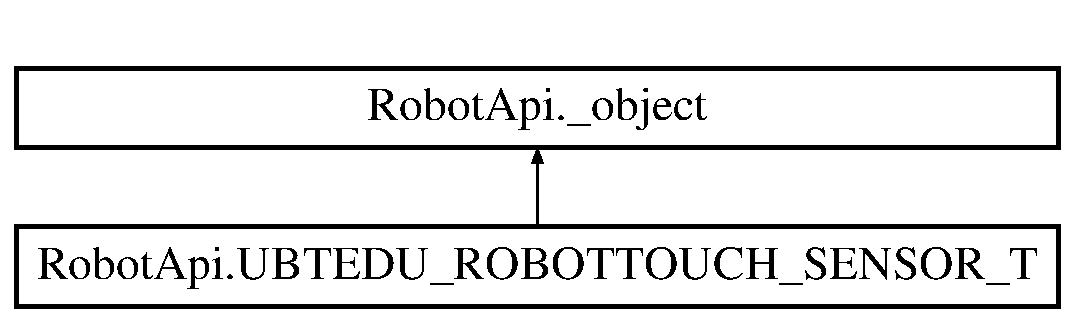
\includegraphics[height=2.000000cm]{classRobotApi_1_1UBTEDU__ROBOTTOUCH__SENSOR__T}
\end{center}
\end{figure}
\subsection*{Public Member Functions}
\begin{DoxyCompactItemize}
\item 
\hypertarget{classRobotApi_1_1UBTEDU__ROBOTTOUCH__SENSOR__T_a578adc374757bf61f2b3f94d7a7cd35e}{def {\bfseries \+\_\+\+\_\+init\+\_\+\+\_\+}}\label{classRobotApi_1_1UBTEDU__ROBOTTOUCH__SENSOR__T_a578adc374757bf61f2b3f94d7a7cd35e}

\end{DoxyCompactItemize}
\subsection*{Public Attributes}
\begin{DoxyCompactItemize}
\item 
\hypertarget{classRobotApi_1_1UBTEDU__ROBOTTOUCH__SENSOR__T_a6620a28cac3af1fb80a2c779c287e597}{{\bfseries this}}\label{classRobotApi_1_1UBTEDU__ROBOTTOUCH__SENSOR__T_a6620a28cac3af1fb80a2c779c287e597}

\end{DoxyCompactItemize}


The documentation for this class was generated from the following file\+:\begin{DoxyCompactItemize}
\item 
Robot\+Api.\+py\end{DoxyCompactItemize}

\hypertarget{classRobotApi_1_1UBTEDU__ROBOTULTRASONIC__SENSOR__T}{\section{Robot\+Api.\+U\+B\+T\+E\+D\+U\+\_\+\+R\+O\+B\+O\+T\+U\+L\+T\+R\+A\+S\+O\+N\+I\+C\+\_\+\+S\+E\+N\+S\+O\+R\+\_\+\+T Class Reference}
\label{classRobotApi_1_1UBTEDU__ROBOTULTRASONIC__SENSOR__T}\index{Robot\+Api.\+U\+B\+T\+E\+D\+U\+\_\+\+R\+O\+B\+O\+T\+U\+L\+T\+R\+A\+S\+O\+N\+I\+C\+\_\+\+S\+E\+N\+S\+O\+R\+\_\+\+T@{Robot\+Api.\+U\+B\+T\+E\+D\+U\+\_\+\+R\+O\+B\+O\+T\+U\+L\+T\+R\+A\+S\+O\+N\+I\+C\+\_\+\+S\+E\+N\+S\+O\+R\+\_\+\+T}}
}
Inheritance diagram for Robot\+Api.\+U\+B\+T\+E\+D\+U\+\_\+\+R\+O\+B\+O\+T\+U\+L\+T\+R\+A\+S\+O\+N\+I\+C\+\_\+\+S\+E\+N\+S\+O\+R\+\_\+\+T\+:\begin{figure}[H]
\begin{center}
\leavevmode
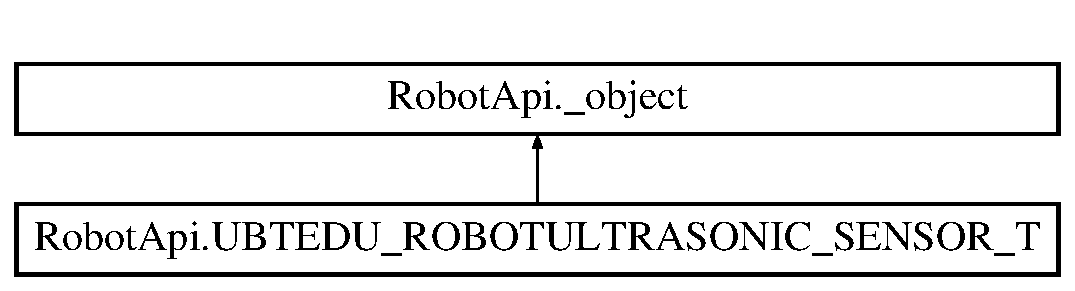
\includegraphics[height=2.000000cm]{classRobotApi_1_1UBTEDU__ROBOTULTRASONIC__SENSOR__T}
\end{center}
\end{figure}
\subsection*{Public Member Functions}
\begin{DoxyCompactItemize}
\item 
\hypertarget{classRobotApi_1_1UBTEDU__ROBOTULTRASONIC__SENSOR__T_ae9a80c764b0ddf164115b236efe19967}{def {\bfseries \+\_\+\+\_\+init\+\_\+\+\_\+}}\label{classRobotApi_1_1UBTEDU__ROBOTULTRASONIC__SENSOR__T_ae9a80c764b0ddf164115b236efe19967}

\end{DoxyCompactItemize}
\subsection*{Public Attributes}
\begin{DoxyCompactItemize}
\item 
\hypertarget{classRobotApi_1_1UBTEDU__ROBOTULTRASONIC__SENSOR__T_a7b83fa3c4a57a14ed367dc3a6e5e9cc0}{{\bfseries this}}\label{classRobotApi_1_1UBTEDU__ROBOTULTRASONIC__SENSOR__T_a7b83fa3c4a57a14ed367dc3a6e5e9cc0}

\end{DoxyCompactItemize}


The documentation for this class was generated from the following file\+:\begin{DoxyCompactItemize}
\item 
Robot\+Api.\+py\end{DoxyCompactItemize}

\hypertarget{classtest__sensor_1_1UbtRobotColor}{\section{test\+\_\+sensor.\+Ubt\+Robot\+Color Class Reference}
\label{classtest__sensor_1_1UbtRobotColor}\index{test\+\_\+sensor.\+Ubt\+Robot\+Color@{test\+\_\+sensor.\+Ubt\+Robot\+Color}}
}
Inheritance diagram for test\+\_\+sensor.\+Ubt\+Robot\+Color\+:\begin{figure}[H]
\begin{center}
\leavevmode
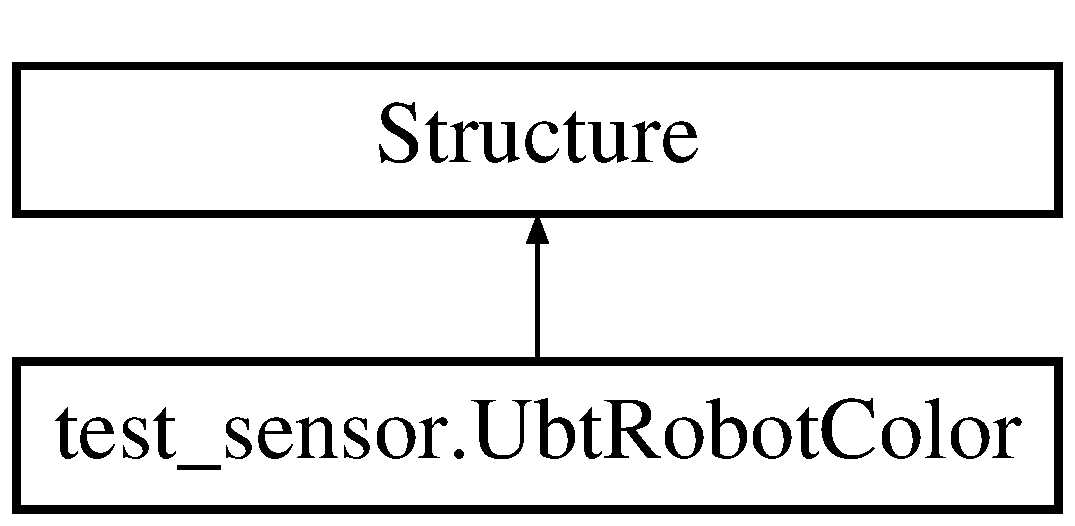
\includegraphics[height=2.000000cm]{classtest__sensor_1_1UbtRobotColor}
\end{center}
\end{figure}


The documentation for this class was generated from the following file\+:\begin{DoxyCompactItemize}
\item 
test\+\_\+sensor.\+py\end{DoxyCompactItemize}

\hypertarget{classtest__sensor_1_1UbtRobotIRorUltrasonic}{\section{test\+\_\+sensor.\+Ubt\+Robot\+I\+Ror\+Ultrasonic Class Reference}
\label{classtest__sensor_1_1UbtRobotIRorUltrasonic}\index{test\+\_\+sensor.\+Ubt\+Robot\+I\+Ror\+Ultrasonic@{test\+\_\+sensor.\+Ubt\+Robot\+I\+Ror\+Ultrasonic}}
}
Inheritance diagram for test\+\_\+sensor.\+Ubt\+Robot\+I\+Ror\+Ultrasonic\+:\begin{figure}[H]
\begin{center}
\leavevmode
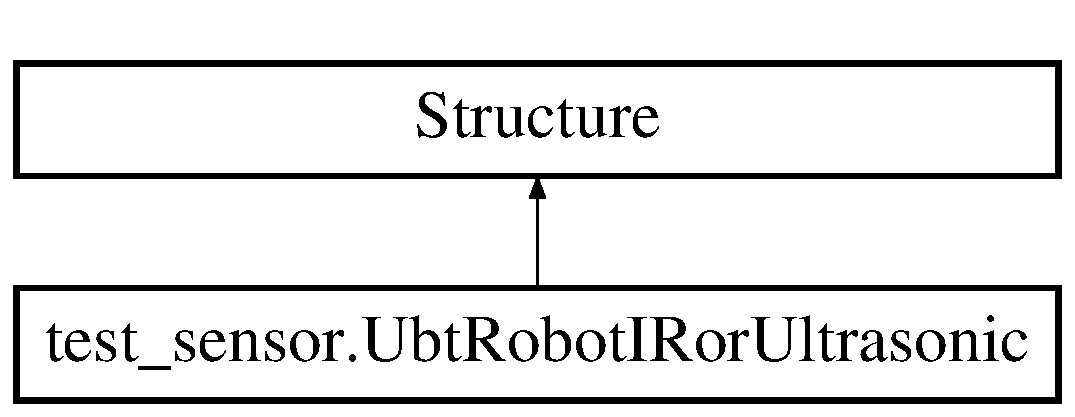
\includegraphics[height=2.000000cm]{classtest__sensor_1_1UbtRobotIRorUltrasonic}
\end{center}
\end{figure}


The documentation for this class was generated from the following file\+:\begin{DoxyCompactItemize}
\item 
test\+\_\+sensor.\+py\end{DoxyCompactItemize}

\hypertarget{classtest__sensor_1_1UbtRobotTemperature}{\section{test\+\_\+sensor.\+Ubt\+Robot\+Temperature Class Reference}
\label{classtest__sensor_1_1UbtRobotTemperature}\index{test\+\_\+sensor.\+Ubt\+Robot\+Temperature@{test\+\_\+sensor.\+Ubt\+Robot\+Temperature}}
}
Inheritance diagram for test\+\_\+sensor.\+Ubt\+Robot\+Temperature\+:\begin{figure}[H]
\begin{center}
\leavevmode
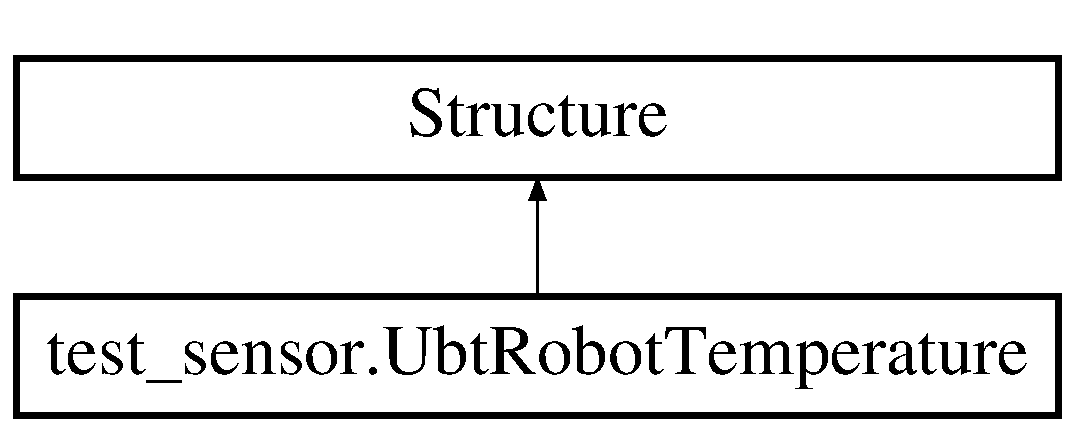
\includegraphics[height=2.000000cm]{classtest__sensor_1_1UbtRobotTemperature}
\end{center}
\end{figure}


The documentation for this class was generated from the following file\+:\begin{DoxyCompactItemize}
\item 
test\+\_\+sensor.\+py\end{DoxyCompactItemize}

\chapter{File Documentation}
\hypertarget{RobotApi_8h}{\section{Robot\+Api.\+h File Reference}
\label{RobotApi_8h}\index{Robot\+Api.\+h@{Robot\+Api.\+h}}
}


Defines the A\+P\+Is for U\+B\+T\+E\+D\+U S\+D\+K.  


\subsection*{Classes}
\begin{DoxyCompactItemize}
\item 
struct \hyperlink{struct__RobotInfo}{\+\_\+\+Robot\+Info}
\begin{DoxyCompactList}\small\item\em Robot infomation. \end{DoxyCompactList}\item 
struct \hyperlink{struct__RobotGyroSensor}{\+\_\+\+Robot\+Gyro\+Sensor}
\begin{DoxyCompactList}\small\item\em Gyro sensor data. \end{DoxyCompactList}\item 
struct \hyperlink{struct__RobotEnvSensor}{\+\_\+\+Robot\+Env\+Sensor}
\begin{DoxyCompactList}\small\item\em Environment sensor data. \end{DoxyCompactList}\item 
struct \hyperlink{struct__RobotRaspPiBoardSensor}{\+\_\+\+Robot\+Rasp\+Pi\+Board\+Sensor}
\begin{DoxyCompactList}\small\item\em Raspberry Pi board P\+C\+B data. \end{DoxyCompactList}\item 
struct \hyperlink{struct__RobotUltrasonicSensor}{\+\_\+\+Robot\+Ultrasonic\+Sensor}
\begin{DoxyCompactList}\small\item\em Ultrasonic sensor data. \end{DoxyCompactList}\item 
struct \hyperlink{struct__RobotInfraredSensor}{\+\_\+\+Robot\+Infrared\+Sensor}
\begin{DoxyCompactList}\small\item\em Infrared sensor data. \end{DoxyCompactList}\item 
struct \hyperlink{struct__RobotTouchSensor}{\+\_\+\+Robot\+Touch\+Sensor}
\begin{DoxyCompactList}\small\item\em Touch sensor data. \end{DoxyCompactList}\item 
struct \hyperlink{struct__RobotColorSensor}{\+\_\+\+Robot\+Color\+Sensor}
\begin{DoxyCompactList}\small\item\em Color sensor data. \end{DoxyCompactList}\item 
struct \hyperlink{struct__RobotPressureSensor}{\+\_\+\+Robot\+Pressure\+Sensor}
\begin{DoxyCompactList}\small\item\em Pressure sensor data. \end{DoxyCompactList}\item 
struct \hyperlink{struct__RobotBatteryInfo}{\+\_\+\+Robot\+Battery\+Info}
\begin{DoxyCompactList}\small\item\em Battery data. \end{DoxyCompactList}\end{DoxyCompactItemize}
\subsection*{Macros}
\begin{DoxyCompactItemize}
\item 
\hypertarget{RobotApi_8h_a15b516e476ff8db35f494b5c3798019b}{\#define {\bfseries U\+B\+T\+E\+D\+U\+\_\+\+S\+D\+K\+\_\+\+S\+W\+\_\+\+V\+E\+R}~\char`\"{}01\char`\"{}}\label{RobotApi_8h_a15b516e476ff8db35f494b5c3798019b}

\item 
\hypertarget{RobotApi_8h_aa37c5da3aea28e1d6eb93c3950ac7afe}{\#define {\bfseries U\+B\+T\+E\+D\+U\+\_\+\+R\+O\+B\+O\+T\+\_\+\+N\+A\+M\+E\+\_\+\+L\+E\+N}~(32)}\label{RobotApi_8h_aa37c5da3aea28e1d6eb93c3950ac7afe}

\item 
\hypertarget{RobotApi_8h_ab92db2df9ca7c3c48ff6495f9bafc53d}{\#define {\bfseries U\+B\+T\+E\+D\+U\+\_\+\+R\+O\+B\+O\+T\+\_\+\+I\+P\+\_\+\+A\+D\+D\+R\+\_\+\+L\+E\+N}~(16)}\label{RobotApi_8h_ab92db2df9ca7c3c48ff6495f9bafc53d}

\end{DoxyCompactItemize}
\subsection*{Typedefs}
\begin{DoxyCompactItemize}
\item 
\hypertarget{RobotApi_8h_aec43ee444eec81491d46180fa38d026f}{typedef struct \hyperlink{struct__RobotInfo}{\+\_\+\+Robot\+Info} \hyperlink{RobotApi_8h_aec43ee444eec81491d46180fa38d026f}{U\+B\+T\+E\+D\+U\+\_\+\+R\+O\+B\+O\+T\+I\+N\+F\+O\+\_\+\+T}}\label{RobotApi_8h_aec43ee444eec81491d46180fa38d026f}

\begin{DoxyCompactList}\small\item\em Robot infomation. \end{DoxyCompactList}\item 
\hypertarget{RobotApi_8h_a6530e7a3744e308a5495914fc2e26b73}{typedef struct \hyperlink{struct__RobotGyroSensor}{\+\_\+\+Robot\+Gyro\+Sensor} \hyperlink{RobotApi_8h_a6530e7a3744e308a5495914fc2e26b73}{U\+B\+T\+E\+D\+U\+\_\+\+R\+O\+B\+O\+T\+G\+Y\+R\+O\+\_\+\+S\+E\+N\+S\+O\+R\+\_\+\+T}}\label{RobotApi_8h_a6530e7a3744e308a5495914fc2e26b73}

\begin{DoxyCompactList}\small\item\em Gyro sensor data. \end{DoxyCompactList}\item 
\hypertarget{RobotApi_8h_ad93975c97078d87731b629c7b8181a41}{typedef struct \hyperlink{struct__RobotEnvSensor}{\+\_\+\+Robot\+Env\+Sensor} \hyperlink{RobotApi_8h_ad93975c97078d87731b629c7b8181a41}{U\+B\+T\+E\+D\+U\+\_\+\+R\+O\+B\+O\+T\+E\+N\+V\+\_\+\+S\+E\+N\+S\+O\+R\+\_\+\+T}}\label{RobotApi_8h_ad93975c97078d87731b629c7b8181a41}

\begin{DoxyCompactList}\small\item\em Environment sensor data. \end{DoxyCompactList}\item 
\hypertarget{RobotApi_8h_ab827cd9f248532706aa7be6ab2c6ffd7}{typedef struct \\*
\hyperlink{struct__RobotRaspPiBoardSensor}{\+\_\+\+Robot\+Rasp\+Pi\+Board\+Sensor} \hyperlink{RobotApi_8h_ab827cd9f248532706aa7be6ab2c6ffd7}{U\+B\+T\+E\+D\+U\+\_\+\+R\+O\+B\+O\+T\+R\+A\+S\+P\+B\+O\+A\+R\+D\+\_\+\+S\+E\+N\+S\+O\+R\+\_\+\+T}}\label{RobotApi_8h_ab827cd9f248532706aa7be6ab2c6ffd7}

\begin{DoxyCompactList}\small\item\em Raspberry Pi board P\+C\+B data. \end{DoxyCompactList}\item 
\hypertarget{RobotApi_8h_ac2eaadaaab9f4e45b0d0aa5c6f9ccef1}{typedef struct \\*
\hyperlink{struct__RobotUltrasonicSensor}{\+\_\+\+Robot\+Ultrasonic\+Sensor} \hyperlink{RobotApi_8h_ac2eaadaaab9f4e45b0d0aa5c6f9ccef1}{U\+B\+T\+E\+D\+U\+\_\+\+R\+O\+B\+O\+T\+U\+L\+T\+R\+A\+S\+O\+N\+I\+C\+\_\+\+S\+E\+N\+S\+O\+R\+\_\+\+T}}\label{RobotApi_8h_ac2eaadaaab9f4e45b0d0aa5c6f9ccef1}

\begin{DoxyCompactList}\small\item\em Ultrasonic sensor data. \end{DoxyCompactList}\item 
\hypertarget{RobotApi_8h_af2269dce746b3ed577df46f1eb2765bb}{typedef struct \hyperlink{struct__RobotInfraredSensor}{\+\_\+\+Robot\+Infrared\+Sensor} \hyperlink{RobotApi_8h_af2269dce746b3ed577df46f1eb2765bb}{U\+B\+T\+E\+D\+U\+\_\+\+R\+O\+B\+O\+T\+I\+N\+F\+R\+A\+R\+E\+D\+\_\+\+S\+E\+N\+S\+O\+R\+\_\+\+T}}\label{RobotApi_8h_af2269dce746b3ed577df46f1eb2765bb}

\begin{DoxyCompactList}\small\item\em Infrared sensor data. \end{DoxyCompactList}\item 
\hypertarget{RobotApi_8h_ac8ffd64e9702593f3a678988f0de9999}{typedef struct \hyperlink{struct__RobotTouchSensor}{\+\_\+\+Robot\+Touch\+Sensor} \hyperlink{RobotApi_8h_ac8ffd64e9702593f3a678988f0de9999}{U\+B\+T\+E\+D\+U\+\_\+\+R\+O\+B\+O\+T\+T\+O\+U\+C\+H\+\_\+\+S\+E\+N\+S\+O\+R\+\_\+\+T}}\label{RobotApi_8h_ac8ffd64e9702593f3a678988f0de9999}

\begin{DoxyCompactList}\small\item\em Touch sensor data. \end{DoxyCompactList}\item 
\hypertarget{RobotApi_8h_aa4969c3b258bf80329c2e1d9f9847e5f}{typedef struct \hyperlink{struct__RobotColorSensor}{\+\_\+\+Robot\+Color\+Sensor} \hyperlink{RobotApi_8h_aa4969c3b258bf80329c2e1d9f9847e5f}{U\+B\+T\+E\+D\+U\+\_\+\+R\+O\+B\+O\+T\+C\+O\+L\+O\+R\+\_\+\+S\+E\+N\+S\+O\+R\+\_\+\+T}}\label{RobotApi_8h_aa4969c3b258bf80329c2e1d9f9847e5f}

\begin{DoxyCompactList}\small\item\em Color sensor data. \end{DoxyCompactList}\item 
\hypertarget{RobotApi_8h_a7e229b309624e28e4b77490561d33ae2}{typedef struct \hyperlink{struct__RobotPressureSensor}{\+\_\+\+Robot\+Pressure\+Sensor} \hyperlink{RobotApi_8h_a7e229b309624e28e4b77490561d33ae2}{U\+B\+T\+E\+D\+U\+\_\+\+R\+O\+B\+O\+T\+P\+R\+E\+S\+S\+U\+R\+E\+\_\+\+S\+E\+N\+S\+O\+R\+\_\+\+T}}\label{RobotApi_8h_a7e229b309624e28e4b77490561d33ae2}

\begin{DoxyCompactList}\small\item\em Pressure sensor data. \end{DoxyCompactList}\item 
\hypertarget{RobotApi_8h_af218f419d970f10bef9d636eefa34849}{typedef struct \hyperlink{struct__RobotBatteryInfo}{\+\_\+\+Robot\+Battery\+Info} \hyperlink{RobotApi_8h_af218f419d970f10bef9d636eefa34849}{U\+B\+T\+E\+D\+U\+\_\+\+R\+O\+B\+O\+T\+\_\+\+Battery\+\_\+\+T}}\label{RobotApi_8h_af218f419d970f10bef9d636eefa34849}

\begin{DoxyCompactList}\small\item\em Battery data. \end{DoxyCompactList}\end{DoxyCompactItemize}
\subsection*{Enumerations}
\begin{DoxyCompactItemize}
\item 
enum \hyperlink{RobotApi_8h_a6cc1b3e4bfe755450bf224e8a79d5278}{U\+B\+T\+E\+D\+U\+\_\+\+R\+O\+B\+O\+T\+\_\+\+S\+T\+A\+T\+U\+S\+\_\+\+T\+Y\+P\+E\+\_\+e} \{ \\*
\hyperlink{RobotApi_8h_a6cc1b3e4bfe755450bf224e8a79d5278a3b91081b4fc4bcfaaa7ec882914a4ec1}{U\+B\+T\+E\+D\+U\+\_\+\+R\+O\+B\+O\+T\+\_\+\+S\+T\+A\+T\+U\+S\+\_\+\+T\+Y\+P\+E\+\_\+\+P\+L\+A\+Y\+A\+C\+T\+I\+O\+N} = 1, 
\hyperlink{RobotApi_8h_a6cc1b3e4bfe755450bf224e8a79d5278a23dc19fd2ef5c7e31071238a0392f65b}{U\+B\+T\+E\+D\+U\+\_\+\+R\+O\+B\+O\+T\+\_\+\+S\+T\+A\+T\+U\+S\+\_\+\+T\+Y\+P\+E\+\_\+\+V\+O\+L\+U\+M\+E}, 
\hyperlink{RobotApi_8h_a6cc1b3e4bfe755450bf224e8a79d5278a89edce1dbe8ac63336cdfb507e9f7b32}{U\+B\+T\+E\+D\+U\+\_\+\+R\+O\+B\+O\+T\+\_\+\+S\+T\+A\+T\+U\+S\+\_\+\+T\+Y\+P\+E\+\_\+\+P\+O\+W\+E\+R\+\_\+\+V\+O\+L\+T\+A\+G\+E}, 
\hyperlink{RobotApi_8h_a6cc1b3e4bfe755450bf224e8a79d5278ab5bd6574e0e272623c8491878eaf615f}{U\+B\+T\+E\+D\+U\+\_\+\+R\+O\+B\+O\+T\+\_\+\+S\+T\+A\+T\+U\+S\+\_\+\+T\+Y\+P\+E\+\_\+\+P\+O\+W\+E\+R\+\_\+\+R\+E\+C\+H\+A\+R\+G\+E}, 
\\*
\hyperlink{RobotApi_8h_a6cc1b3e4bfe755450bf224e8a79d5278ae5d6b683955aa924ab8ea32d5bf04741}{U\+B\+T\+E\+D\+U\+\_\+\+R\+O\+B\+O\+T\+\_\+\+S\+T\+A\+T\+U\+S\+\_\+\+T\+Y\+P\+E\+\_\+\+P\+O\+W\+E\+R\+\_\+\+P\+E\+R\+C\+E\+N\+T}, 
\hyperlink{RobotApi_8h_a6cc1b3e4bfe755450bf224e8a79d5278acfbf49ba0ca676aed962376dd63daca6}{U\+B\+T\+E\+D\+U\+\_\+\+R\+O\+B\+O\+T\+\_\+\+S\+T\+A\+T\+U\+S\+\_\+\+T\+Y\+P\+E\+\_\+\+P\+O\+W\+E\+R\+\_\+\+L\+O\+W\+A\+L\+E\+R\+T}, 
\hyperlink{RobotApi_8h_a6cc1b3e4bfe755450bf224e8a79d5278a18599f77d706c9bb64dcb20696fe2d32}{U\+B\+T\+E\+D\+U\+\_\+\+R\+O\+B\+O\+T\+\_\+\+S\+T\+A\+T\+U\+S\+\_\+\+T\+Y\+P\+E\+\_\+\+I\+N\+V\+A\+L\+I\+D}
 \}
\begin{DoxyCompactList}\small\item\em Robot status type. \end{DoxyCompactList}\item 
enum \hyperlink{RobotApi_8h_aa1a4cf8082958a664cf36c2f1638fb46}{U\+B\+T\+E\+D\+U\+\_\+\+R\+O\+B\+O\+T\+\_\+\+P\+L\+A\+Y\+M\+U\+S\+I\+C\+\_\+\+S\+T\+A\+T\+U\+S\+\_\+e} \{ \\*
\hyperlink{RobotApi_8h_aa1a4cf8082958a664cf36c2f1638fb46a5350aa0b01ece30898e03c112fa90a80}{U\+B\+T\+E\+D\+U\+\_\+\+R\+O\+B\+O\+T\+\_\+\+P\+L\+A\+Y\+\_\+\+S\+T\+A\+T\+U\+S\+\_\+\+I\+D\+L\+E}, 
\hyperlink{RobotApi_8h_aa1a4cf8082958a664cf36c2f1638fb46ad25b97955eb307910d7ca17a0c50b792}{U\+B\+T\+E\+D\+U\+\_\+\+R\+O\+B\+O\+T\+\_\+\+P\+L\+A\+Y\+\_\+\+S\+T\+A\+T\+U\+S\+\_\+\+P\+L\+A\+Y\+I\+N\+G}, 
\hyperlink{RobotApi_8h_aa1a4cf8082958a664cf36c2f1638fb46a084466c986785a392db3c343c805b650}{U\+B\+T\+E\+D\+U\+\_\+\+R\+O\+B\+O\+T\+\_\+\+P\+L\+A\+Y\+\_\+\+S\+T\+A\+T\+U\+S\+\_\+\+P\+A\+U\+S\+E\+D}, 
\hyperlink{RobotApi_8h_aa1a4cf8082958a664cf36c2f1638fb46a0632b70d2578990a9145b0d99a89660c}{U\+B\+T\+E\+D\+U\+\_\+\+R\+O\+B\+O\+T\+\_\+\+P\+L\+A\+Y\+S\+T\+A\+T\+U\+S\+\_\+\+E\+N\+D}, 
\\*
\hyperlink{RobotApi_8h_aa1a4cf8082958a664cf36c2f1638fb46a4d407ef9e493dd6560961237d617a3b2}{U\+B\+T\+E\+D\+U\+\_\+\+R\+O\+B\+O\+T\+\_\+\+P\+L\+A\+Y\+\_\+\+S\+T\+A\+T\+U\+S\+\_\+\+I\+N\+V\+A\+L\+I\+D}
 \}
\begin{DoxyCompactList}\small\item\em Play music status. \end{DoxyCompactList}\item 
enum \hyperlink{RobotApi_8h_acf968c25155e4858eb86474d572f5545}{U\+B\+T\+E\+D\+U\+\_\+\+R\+O\+B\+O\+T\+\_\+\+S\+O\+F\+T\+V\+E\+R\+S\+I\+O\+N\+\_\+\+T\+Y\+P\+E\+\_\+e} \{ \\*
\hyperlink{RobotApi_8h_acf968c25155e4858eb86474d572f5545a66fc95118444744d3b6febdfd847814a}{U\+B\+T\+E\+D\+U\+\_\+\+R\+O\+B\+O\+T\+\_\+\+S\+O\+F\+T\+V\+E\+R\+S\+I\+O\+N\+\_\+\+T\+Y\+P\+E\+\_\+\+S\+T\+M32} = 0, 
\hyperlink{RobotApi_8h_acf968c25155e4858eb86474d572f5545aaea68ee7b7b11575126b7540542bde09}{U\+B\+T\+E\+D\+U\+\_\+\+R\+O\+B\+O\+T\+\_\+\+S\+O\+F\+T\+V\+E\+R\+S\+I\+O\+N\+\_\+\+T\+Y\+P\+E\+\_\+\+S\+E\+R\+V\+O\+S1}, 
{\bfseries U\+B\+T\+E\+D\+U\+\_\+\+R\+O\+B\+O\+T\+\_\+\+S\+O\+F\+T\+V\+E\+R\+S\+I\+O\+N\+\_\+\+T\+Y\+P\+E\+\_\+\+S\+E\+R\+V\+O\+S2}, 
{\bfseries U\+B\+T\+E\+D\+U\+\_\+\+R\+O\+B\+O\+T\+\_\+\+S\+O\+F\+T\+V\+E\+R\+S\+I\+O\+N\+\_\+\+T\+Y\+P\+E\+\_\+\+S\+E\+R\+V\+O\+S3}, 
\\*
{\bfseries U\+B\+T\+E\+D\+U\+\_\+\+R\+O\+B\+O\+T\+\_\+\+S\+O\+F\+T\+V\+E\+R\+S\+I\+O\+N\+\_\+\+T\+Y\+P\+E\+\_\+\+S\+E\+R\+V\+O\+S4}, 
{\bfseries U\+B\+T\+E\+D\+U\+\_\+\+R\+O\+B\+O\+T\+\_\+\+S\+O\+F\+T\+V\+E\+R\+S\+I\+O\+N\+\_\+\+T\+Y\+P\+E\+\_\+\+S\+E\+R\+V\+O\+S5}, 
{\bfseries U\+B\+T\+E\+D\+U\+\_\+\+R\+O\+B\+O\+T\+\_\+\+S\+O\+F\+T\+V\+E\+R\+S\+I\+O\+N\+\_\+\+T\+Y\+P\+E\+\_\+\+S\+E\+R\+V\+O\+S6}, 
{\bfseries U\+B\+T\+E\+D\+U\+\_\+\+R\+O\+B\+O\+T\+\_\+\+S\+O\+F\+T\+V\+E\+R\+S\+I\+O\+N\+\_\+\+T\+Y\+P\+E\+\_\+\+S\+E\+R\+V\+O\+S7}, 
\\*
{\bfseries U\+B\+T\+E\+D\+U\+\_\+\+R\+O\+B\+O\+T\+\_\+\+S\+O\+F\+T\+V\+E\+R\+S\+I\+O\+N\+\_\+\+T\+Y\+P\+E\+\_\+\+S\+E\+R\+V\+O\+S8}, 
{\bfseries U\+B\+T\+E\+D\+U\+\_\+\+R\+O\+B\+O\+T\+\_\+\+S\+O\+F\+T\+V\+E\+R\+S\+I\+O\+N\+\_\+\+T\+Y\+P\+E\+\_\+\+S\+E\+R\+V\+O\+S9}, 
{\bfseries U\+B\+T\+E\+D\+U\+\_\+\+R\+O\+B\+O\+T\+\_\+\+S\+O\+F\+T\+V\+E\+R\+S\+I\+O\+N\+\_\+\+T\+Y\+P\+E\+\_\+\+S\+E\+R\+V\+O\+S10}, 
{\bfseries U\+B\+T\+E\+D\+U\+\_\+\+R\+O\+B\+O\+T\+\_\+\+S\+O\+F\+T\+V\+E\+R\+S\+I\+O\+N\+\_\+\+T\+Y\+P\+E\+\_\+\+S\+E\+R\+V\+O\+S11}, 
\\*
{\bfseries U\+B\+T\+E\+D\+U\+\_\+\+R\+O\+B\+O\+T\+\_\+\+S\+O\+F\+T\+V\+E\+R\+S\+I\+O\+N\+\_\+\+T\+Y\+P\+E\+\_\+\+S\+E\+R\+V\+O\+S12}, 
{\bfseries U\+B\+T\+E\+D\+U\+\_\+\+R\+O\+B\+O\+T\+\_\+\+S\+O\+F\+T\+V\+E\+R\+S\+I\+O\+N\+\_\+\+T\+Y\+P\+E\+\_\+\+S\+E\+R\+V\+O\+S13}, 
{\bfseries U\+B\+T\+E\+D\+U\+\_\+\+R\+O\+B\+O\+T\+\_\+\+S\+O\+F\+T\+V\+E\+R\+S\+I\+O\+N\+\_\+\+T\+Y\+P\+E\+\_\+\+S\+E\+R\+V\+O\+S14}, 
{\bfseries U\+B\+T\+E\+D\+U\+\_\+\+R\+O\+B\+O\+T\+\_\+\+S\+O\+F\+T\+V\+E\+R\+S\+I\+O\+N\+\_\+\+T\+Y\+P\+E\+\_\+\+S\+E\+R\+V\+O\+S15}, 
\\*
{\bfseries U\+B\+T\+E\+D\+U\+\_\+\+R\+O\+B\+O\+T\+\_\+\+S\+O\+F\+T\+V\+E\+R\+S\+I\+O\+N\+\_\+\+T\+Y\+P\+E\+\_\+\+S\+E\+R\+V\+O\+S16}, 
{\bfseries U\+B\+T\+E\+D\+U\+\_\+\+R\+O\+B\+O\+T\+\_\+\+S\+O\+F\+T\+V\+E\+R\+S\+I\+O\+N\+\_\+\+T\+Y\+P\+E\+\_\+\+S\+E\+R\+V\+O\+S17}, 
\hyperlink{RobotApi_8h_acf968c25155e4858eb86474d572f5545a013da89dfee673d5362e986dcf458979}{U\+B\+T\+E\+D\+U\+\_\+\+R\+O\+B\+O\+T\+\_\+\+S\+O\+F\+T\+V\+E\+R\+S\+I\+O\+N\+\_\+\+T\+Y\+P\+E\+\_\+\+S\+D\+K} = 30, 
\hyperlink{RobotApi_8h_acf968c25155e4858eb86474d572f5545a18801a2935ecc0bbed27c232c914150c}{U\+B\+T\+E\+D\+U\+\_\+\+R\+O\+B\+O\+T\+\_\+\+S\+O\+F\+T\+V\+E\+R\+S\+I\+O\+N\+\_\+\+T\+Y\+P\+E\+\_\+\+R\+A\+S\+P\+I} = 31, 
\\*
\hyperlink{RobotApi_8h_acf968c25155e4858eb86474d572f5545a9c6c01aa83db9d78f3093a50db7cf6b9}{U\+B\+T\+E\+D\+U\+\_\+\+R\+O\+B\+O\+T\+\_\+\+S\+O\+F\+T\+V\+E\+R\+S\+I\+O\+N\+\_\+\+T\+Y\+P\+E\+\_\+\+I\+N\+V\+A\+L\+I\+D}
 \}
\begin{DoxyCompactList}\small\item\em Robot software version type. \end{DoxyCompactList}\item 
enum \hyperlink{RobotApi_8h_a34d32d80f25c4eb5c59fefdebbbefa1c}{U\+B\+T\+E\+D\+U\+\_\+\+R\+C\+\_\+\+T} \{ \\*
\hyperlink{RobotApi_8h_a34d32d80f25c4eb5c59fefdebbbefa1ca768cfa78e26859b81feebb55661d3b41}{U\+B\+T\+E\+D\+U\+\_\+\+R\+C\+\_\+\+S\+U\+C\+C\+E\+S\+S} = 0, 
\hyperlink{RobotApi_8h_a34d32d80f25c4eb5c59fefdebbbefa1ca1f9eb8393ca7033378a8ea30d5948050}{U\+B\+T\+E\+D\+U\+\_\+\+R\+C\+\_\+\+F\+A\+I\+L\+E\+D}, 
\hyperlink{RobotApi_8h_a34d32d80f25c4eb5c59fefdebbbefa1caa564c92f1228107d9e60a684ab5b0618}{U\+B\+T\+E\+D\+U\+\_\+\+R\+C\+\_\+\+N\+O\+R\+E\+S\+O\+U\+R\+C\+E}, 
\hyperlink{RobotApi_8h_a34d32d80f25c4eb5c59fefdebbbefa1cabbd1eb9480997280192083c96bcf6490}{U\+B\+T\+E\+D\+U\+\_\+\+R\+C\+\_\+\+N\+O\+T\+\_\+\+F\+O\+U\+N\+D}, 
\\*
\hyperlink{RobotApi_8h_a34d32d80f25c4eb5c59fefdebbbefa1ca1c558f09747e4187517985362ff7a3c2}{U\+B\+T\+E\+D\+U\+\_\+\+R\+C\+\_\+\+W\+R\+O\+N\+G\+\_\+\+P\+A\+R\+A\+M}, 
\hyperlink{RobotApi_8h_a34d32d80f25c4eb5c59fefdebbbefa1cad15ca9d51da819b6afb7b3c7ab027217}{U\+B\+T\+E\+D\+U\+\_\+\+R\+C\+\_\+\+I\+G\+N\+O\+R\+E}, 
\hyperlink{RobotApi_8h_a34d32d80f25c4eb5c59fefdebbbefa1ca24461f0e778c66ed7bcffce6d7695a11}{U\+B\+T\+E\+D\+U\+\_\+\+R\+C\+\_\+\+S\+O\+C\+K\+E\+T\+\_\+\+F\+A\+I\+L\+E\+D} = 100, 
\hyperlink{RobotApi_8h_a34d32d80f25c4eb5c59fefdebbbefa1caa9723bae0b9970991511d7f57ff87620}{U\+B\+T\+E\+D\+U\+\_\+\+R\+C\+\_\+\+S\+O\+C\+K\+E\+T\+\_\+\+N\+O\+R\+E\+S\+O\+U\+R\+C\+E}, 
\\*
\hyperlink{RobotApi_8h_a34d32d80f25c4eb5c59fefdebbbefa1ca79a22ff9360807f60f03e2dbf9143ffc}{U\+B\+T\+E\+D\+U\+\_\+\+R\+C\+\_\+\+S\+O\+C\+K\+E\+T\+\_\+\+T\+I\+M\+E\+O\+U\+T}, 
\hyperlink{RobotApi_8h_a34d32d80f25c4eb5c59fefdebbbefa1ca99307d6318a6ed53f617ed1cd493df0c}{U\+B\+T\+E\+D\+U\+\_\+\+R\+C\+\_\+\+S\+O\+C\+K\+E\+T\+\_\+\+E\+N\+C\+O\+D\+E\+\_\+\+F\+A\+I\+L\+E\+D}, 
\hyperlink{RobotApi_8h_a34d32d80f25c4eb5c59fefdebbbefa1ca17e62780695ac1078a402bf294681b72}{U\+B\+T\+E\+D\+U\+\_\+\+R\+C\+\_\+\+S\+O\+C\+K\+E\+T\+\_\+\+D\+E\+C\+O\+D\+E\+\_\+\+F\+A\+I\+L\+E\+D}, 
\hyperlink{RobotApi_8h_a34d32d80f25c4eb5c59fefdebbbefa1ca7527e9660579b5229728384a63b66a7f}{U\+B\+T\+E\+D\+U\+\_\+\+R\+C\+\_\+\+S\+O\+C\+K\+E\+T\+\_\+\+E\+N\+C\+O\+D\+E\+\_\+\+E\+R\+R\+O\+R}, 
\\*
\hyperlink{RobotApi_8h_a34d32d80f25c4eb5c59fefdebbbefa1ca740c8d6d936049c5116690439a3212c0}{U\+B\+T\+E\+D\+U\+\_\+\+R\+C\+\_\+\+S\+O\+C\+K\+E\+T\+\_\+\+D\+E\+C\+O\+D\+E\+\_\+\+E\+R\+R\+O\+R}, 
\hyperlink{RobotApi_8h_a34d32d80f25c4eb5c59fefdebbbefa1caa4c594bb02be4941e384d586b3e991e1}{U\+B\+T\+E\+D\+U\+\_\+\+R\+C\+\_\+\+S\+O\+C\+K\+E\+T\+\_\+\+S\+E\+N\+D\+E\+R\+R\+O\+R}, 
\hyperlink{RobotApi_8h_a34d32d80f25c4eb5c59fefdebbbefa1ca4c6c318f650d422ce9d1a562e9282722}{U\+B\+T\+E\+D\+U\+\_\+\+R\+C\+\_\+\+V\+O\+I\+C\+E\+\_\+\+F\+A\+I\+L\+E\+D}, 
\hyperlink{RobotApi_8h_a34d32d80f25c4eb5c59fefdebbbefa1ca96680e77719482c73f029aed67ac10f0}{U\+B\+T\+E\+D\+U\+\_\+\+R\+C\+\_\+\+V\+O\+I\+C\+E\+\_\+\+G\+R\+A\+M\+M\+A\+R\+\_\+\+E\+R\+R\+O\+R}, 
\\*
\hyperlink{RobotApi_8h_a34d32d80f25c4eb5c59fefdebbbefa1cacce0b6bf8adb079c9705a4a75686e817}{U\+B\+T\+E\+D\+U\+\_\+\+R\+C\+\_\+\+V\+O\+I\+C\+E\+\_\+\+A\+I\+U\+I\+D\+E\+C\+O\+D\+E\+\_\+\+E\+R\+R\+O\+R}, 
\hyperlink{RobotApi_8h_a34d32d80f25c4eb5c59fefdebbbefa1ca1ab6a8ee17053a30614fafec64722760}{U\+B\+T\+E\+D\+U\+\_\+\+R\+C\+\_\+\+L\+A\+S\+T}
 \}
\begin{DoxyCompactList}\small\item\em Return value for S\+D\+K. \end{DoxyCompactList}\end{DoxyCompactItemize}
\subsection*{Functions}
\begin{DoxyCompactItemize}
\item 
\hyperlink{RobotApi_8h_a34d32d80f25c4eb5c59fefdebbbefa1c}{U\+B\+T\+E\+D\+U\+\_\+\+R\+C\+\_\+\+T} \hyperlink{RobotApi_8h_a191e38ea22f4c7e6498f513193aec827}{ubt\+Get\+S\+W\+Version} (\hyperlink{RobotApi_8h_acf968c25155e4858eb86474d572f5545}{U\+B\+T\+E\+D\+U\+\_\+\+R\+O\+B\+O\+T\+\_\+\+S\+O\+F\+T\+V\+E\+R\+S\+I\+O\+N\+\_\+\+T\+Y\+P\+E\+\_\+e} e\+Type, char $\ast$pc\+Version, int i\+Version\+Len)
\begin{DoxyCompactList}\small\item\em \+: ubt\+Get\+S\+W\+Version \end{DoxyCompactList}\item 
\hyperlink{RobotApi_8h_a34d32d80f25c4eb5c59fefdebbbefa1c}{U\+B\+T\+E\+D\+U\+\_\+\+R\+C\+\_\+\+T} \hyperlink{RobotApi_8h_a52f54f46cd26849ce64a8dde41844f4b}{ubt\+Get\+Robot\+Status} (\hyperlink{RobotApi_8h_a6cc1b3e4bfe755450bf224e8a79d5278}{U\+B\+T\+E\+D\+U\+\_\+\+R\+O\+B\+O\+T\+\_\+\+S\+T\+A\+T\+U\+S\+\_\+\+T\+Y\+P\+E\+\_\+e} e\+Type, void $\ast$pi\+Status)
\begin{DoxyCompactList}\small\item\em \+: ubt\+Get\+Robot\+Status \end{DoxyCompactList}\item 
\hyperlink{RobotApi_8h_a34d32d80f25c4eb5c59fefdebbbefa1c}{U\+B\+T\+E\+D\+U\+\_\+\+R\+C\+\_\+\+T} \hyperlink{RobotApi_8h_a7b53a39f938f1a62b6c50f4afcee5318}{ubt\+Check\+A\+P\+P\+Status} (char $\ast$pc\+Buf, int i\+Wait\+Time)
\begin{DoxyCompactList}\small\item\em \+: ubt\+Check\+A\+P\+P\+Status \end{DoxyCompactList}\item 
\hyperlink{RobotApi_8h_a34d32d80f25c4eb5c59fefdebbbefa1c}{U\+B\+T\+E\+D\+U\+\_\+\+R\+C\+\_\+\+T} \hyperlink{RobotApi_8h_adc5201d34af3a6c58d60c0d4c9139b0d}{ubt\+Detect\+Voice\+Msg} (char $\ast$pc\+Buf, int i\+Timeout)
\begin{DoxyCompactList}\small\item\em \+: ubt\+Detect\+Voice\+Msg \end{DoxyCompactList}\item 
\hyperlink{RobotApi_8h_a34d32d80f25c4eb5c59fefdebbbefa1c}{U\+B\+T\+E\+D\+U\+\_\+\+R\+C\+\_\+\+T} \hyperlink{RobotApi_8h_a99677753c63095804622d927683e7967}{ubt\+Get\+Robot\+Servo} (int i\+Index\+Mask, char $\ast$pc\+Angle, int i\+Angle\+Len)
\begin{DoxyCompactList}\small\item\em \+: ubt\+Get\+Robot\+Servo \end{DoxyCompactList}\item 
\hyperlink{RobotApi_8h_a34d32d80f25c4eb5c59fefdebbbefa1c}{U\+B\+T\+E\+D\+U\+\_\+\+R\+C\+\_\+\+T} \hyperlink{RobotApi_8h_a5513d1f10534ab2f51e69dfe1efe64d3}{ubt\+Set\+Robot\+Servo} (int i\+Index\+Mask, char $\ast$pc\+Angle, int i\+Time)
\begin{DoxyCompactList}\small\item\em \+: ubt\+Set\+Robot\+Servo \end{DoxyCompactList}\item 
\hyperlink{RobotApi_8h_a34d32d80f25c4eb5c59fefdebbbefa1c}{U\+B\+T\+E\+D\+U\+\_\+\+R\+C\+\_\+\+T} \hyperlink{RobotApi_8h_af8ccd1f17fa7aae1f887f59d5267e764}{ubt\+Set\+Robot\+Volume} (int i\+Volume)
\begin{DoxyCompactList}\small\item\em \+: ubt\+Set\+Robot\+Volume \end{DoxyCompactList}\item 
\hyperlink{RobotApi_8h_a34d32d80f25c4eb5c59fefdebbbefa1c}{U\+B\+T\+E\+D\+U\+\_\+\+R\+C\+\_\+\+T} \hyperlink{RobotApi_8h_a9fd59d5f2541f8fe788cd29f56b1a6ef}{ubt\+Set\+Robot\+Motion} (char $\ast$pc\+Type, char $\ast$pc\+Direct, int i\+Speed, int i\+Repeat)
\begin{DoxyCompactList}\small\item\em \+: ubt\+Set\+Robot\+Motion \end{DoxyCompactList}\item 
\hyperlink{RobotApi_8h_a34d32d80f25c4eb5c59fefdebbbefa1c}{U\+B\+T\+E\+D\+U\+\_\+\+R\+C\+\_\+\+T} \hyperlink{RobotApi_8h_a76ec31fabab2b5baeb25f8ef3781aa1b}{ubt\+Read\+Sensor\+Value} (char $\ast$pc\+Sensor\+Type, void $\ast$p\+Value, int i\+Value\+Len)
\begin{DoxyCompactList}\small\item\em \+: ubt\+Read\+Sensor\+Value \end{DoxyCompactList}\item 
\hyperlink{RobotApi_8h_a34d32d80f25c4eb5c59fefdebbbefa1c}{U\+B\+T\+E\+D\+U\+\_\+\+R\+C\+\_\+\+T} \hyperlink{RobotApi_8h_a730a610c78cbdfbbc67fa2f81ad54156}{ubt\+Read\+Sensor\+Value\+By\+Addr} (char $\ast$pc\+Sensor\+Type, int i\+Addr, void $\ast$p\+Value, int i\+Value\+Len)
\begin{DoxyCompactList}\small\item\em \+: ubt\+Read\+Sensor\+Value\+By\+Addr \end{DoxyCompactList}\item 
\hyperlink{RobotApi_8h_a34d32d80f25c4eb5c59fefdebbbefa1c}{U\+B\+T\+E\+D\+U\+\_\+\+R\+C\+\_\+\+T} \hyperlink{RobotApi_8h_acc97a2d4e5f1db8f355b3c8557d8f7ea}{ubt\+Set\+Robot\+L\+E\+D} (char $\ast$pc\+Type, char $\ast$pc\+Color, char $\ast$pc\+Mode)
\begin{DoxyCompactList}\small\item\em \+: ubt\+Set\+Robot\+L\+E\+D \end{DoxyCompactList}\item 
\hyperlink{RobotApi_8h_a34d32d80f25c4eb5c59fefdebbbefa1c}{U\+B\+T\+E\+D\+U\+\_\+\+R\+C\+\_\+\+T} \hyperlink{RobotApi_8h_a9c0c4870b9aa50e4df36d4615af38eba}{ubt\+Start\+Robot\+Action} (char $\ast$pc\+Name, int i\+Repeat)
\begin{DoxyCompactList}\small\item\em \+: ubt\+Start\+Robot\+Action \end{DoxyCompactList}\item 
\hyperlink{RobotApi_8h_a34d32d80f25c4eb5c59fefdebbbefa1c}{U\+B\+T\+E\+D\+U\+\_\+\+R\+C\+\_\+\+T} \hyperlink{RobotApi_8h_afea679f835ca450290dfcc9500d32c4b}{ubt\+Stop\+Robot\+Action} (void)
\begin{DoxyCompactList}\small\item\em Stop to run the robot action file. \end{DoxyCompactList}\item 
\hyperlink{RobotApi_8h_a34d32d80f25c4eb5c59fefdebbbefa1c}{U\+B\+T\+E\+D\+U\+\_\+\+R\+C\+\_\+\+T} \hyperlink{RobotApi_8h_ad440bc6c26844d90b663ef37c20e1467}{ubt\+Voice\+Start} ()
\begin{DoxyCompactList}\small\item\em Start voice recognition. \end{DoxyCompactList}\item 
\hyperlink{RobotApi_8h_a34d32d80f25c4eb5c59fefdebbbefa1c}{U\+B\+T\+E\+D\+U\+\_\+\+R\+C\+\_\+\+T} \hyperlink{RobotApi_8h_a7b41d83f75fd8d7a88d3110290ab7267}{ubt\+Voice\+Stop} ()
\begin{DoxyCompactList}\small\item\em Stop voice recognition. \end{DoxyCompactList}\item 
\hyperlink{RobotApi_8h_a34d32d80f25c4eb5c59fefdebbbefa1c}{U\+B\+T\+E\+D\+U\+\_\+\+R\+C\+\_\+\+T} \hyperlink{RobotApi_8h_a21536f4d2df601f17bce8f94dc73c0ca}{ubt\+Voice\+T\+T\+S} (int is\+Interrputed, char $\ast$pc\+T\+T\+S)
\begin{DoxyCompactList}\small\item\em Play the T\+T\+S voice. \end{DoxyCompactList}\item 
\hyperlink{RobotApi_8h_a34d32d80f25c4eb5c59fefdebbbefa1c}{U\+B\+T\+E\+D\+U\+\_\+\+R\+C\+\_\+\+T} \hyperlink{RobotApi_8h_a245d75a325f326fcee0e910d2fcd7e4e}{ubt\+Play\+Music} (char $\ast$pc\+Play\+Music\+Type, char $\ast$pc\+Name)
\begin{DoxyCompactList}\small\item\em Play a music. \end{DoxyCompactList}\item 
\hyperlink{RobotApi_8h_a34d32d80f25c4eb5c59fefdebbbefa1c}{U\+B\+T\+E\+D\+U\+\_\+\+R\+C\+\_\+\+T} \hyperlink{RobotApi_8h_aff4c343458f2b2500bc41a9fa2482e84}{ubt\+Get\+Music\+List} (char $\ast$pac\+Music\+Name\mbox{[}$\,$\mbox{]}, int i\+Each\+Music\+Name\+Len, int i\+Music\+Name\+Num, int $\ast$pi\+Index)
\begin{DoxyCompactList}\small\item\em \+: ubt\+Get\+Music\+List \end{DoxyCompactList}\item 
\hyperlink{RobotApi_8h_a34d32d80f25c4eb5c59fefdebbbefa1c}{U\+B\+T\+E\+D\+U\+\_\+\+R\+C\+\_\+\+T} \hyperlink{RobotApi_8h_a43402e9818a3c836d2e0e8c2dc19d147}{ubt\+Vision\+Detect} (char $\ast$pc\+Vision\+Type, char $\ast$pc\+Value, int i\+Timeout)
\begin{DoxyCompactList}\small\item\em \+: ubt\+Vision\+Detect \end{DoxyCompactList}\item 
\hyperlink{RobotApi_8h_a34d32d80f25c4eb5c59fefdebbbefa1c}{U\+B\+T\+E\+D\+U\+\_\+\+R\+C\+\_\+\+T} \hyperlink{RobotApi_8h_a30b29443f869dc93383af4ff61926521}{ubt\+Take\+A\+Photo} (char $\ast$pac\+Photo\+Name, int i\+Photo\+Name\+Len)
\begin{DoxyCompactList}\small\item\em \+: ubt\+Take\+A\+Photo \end{DoxyCompactList}\item 
\hyperlink{RobotApi_8h_a34d32d80f25c4eb5c59fefdebbbefa1c}{U\+B\+T\+E\+D\+U\+\_\+\+R\+C\+\_\+\+T} \hyperlink{RobotApi_8h_a775459a10666a3a4df2eec6125779df4}{ubt\+Transmit\+C\+M\+D} (char $\ast$pc\+Remote\+Cmd, char $\ast$pc\+Remote\+Cmd\+Ret\+Data, int i\+Remote\+Cmd\+Ret\+Data\+Len)
\begin{DoxyCompactList}\small\item\em \+: ubt\+Transmit\+C\+M\+D \end{DoxyCompactList}\item 
\hyperlink{RobotApi_8h_a34d32d80f25c4eb5c59fefdebbbefa1c}{U\+B\+T\+E\+D\+U\+\_\+\+R\+C\+\_\+\+T} \hyperlink{RobotApi_8h_a8909494bc51014a9adcce8f1bec5fbe0}{ubt\+Report\+Status\+To\+App} (char $\ast$pc\+Name, char $\ast$pc\+String)
\begin{DoxyCompactList}\small\item\em Send the Blockly run status to mobile A\+P\+P. \end{DoxyCompactList}\item 
\hyperlink{RobotApi_8h_a34d32d80f25c4eb5c59fefdebbbefa1c}{U\+B\+T\+E\+D\+U\+\_\+\+R\+C\+\_\+\+T} \hyperlink{RobotApi_8h_ac92ca095b201f92bac93081de221bbca}{ubt\+Robot\+Discovery} (int i\+Is\+Need\+Send\+Request, char $\ast$pc\+Account, \hyperlink{RobotApi_8h_aec43ee444eec81491d46180fa38d026f}{U\+B\+T\+E\+D\+U\+\_\+\+R\+O\+B\+O\+T\+I\+N\+F\+O\+\_\+\+T} $\ast$pst\+Robot\+Info)
\begin{DoxyCompactList}\small\item\em \+: ubt\+Robot\+Discovery \end{DoxyCompactList}\item 
\hyperlink{RobotApi_8h_a34d32d80f25c4eb5c59fefdebbbefa1c}{U\+B\+T\+E\+D\+U\+\_\+\+R\+C\+\_\+\+T} \hyperlink{RobotApi_8h_a40990fef7ac2832db71cb09ab38117d7}{ubt\+Robot\+Connect} (char $\ast$pc\+Account, char $\ast$pc\+Version, char $\ast$pc\+I\+P\+Addr)
\begin{DoxyCompactList}\small\item\em \+: ubt\+Robot\+Connect \end{DoxyCompactList}\item 
\hyperlink{RobotApi_8h_a34d32d80f25c4eb5c59fefdebbbefa1c}{U\+B\+T\+E\+D\+U\+\_\+\+R\+C\+\_\+\+T} \hyperlink{RobotApi_8h_af46f3b2657ebc40b2dbded0ad073fccd}{ubt\+Robot\+Disconnect} (char $\ast$pc\+Account, char $\ast$pc\+Version, char $\ast$pc\+I\+P\+Addr)
\begin{DoxyCompactList}\small\item\em \+: ubt\+Robot\+Disconnect \end{DoxyCompactList}\item 
\hyperlink{RobotApi_8h_a34d32d80f25c4eb5c59fefdebbbefa1c}{U\+B\+T\+E\+D\+U\+\_\+\+R\+C\+\_\+\+T} \hyperlink{RobotApi_8h_a2885db6bfcd8e54fb3c6da2506cd620c}{ubt\+Robot\+Initialize} ()
\begin{DoxyCompactList}\small\item\em \+: ubt\+Robot\+Initialize \end{DoxyCompactList}\item 
void \hyperlink{RobotApi_8h_a483ccb40c4ee14564e32d1af0c29fb73}{ubt\+Robot\+Deinitialize} ()
\begin{DoxyCompactList}\small\item\em \+: ubt\+Robot\+Deinitialize \end{DoxyCompactList}\end{DoxyCompactItemize}


\subsection{Detailed Description}
Defines the A\+P\+Is for U\+B\+T\+E\+D\+U S\+D\+K. 

\begin{DoxyNote}{Note}
U\+B\+T Education Co., Ltd. All Right Reserved. 
\end{DoxyNote}
\begin{DoxyAuthor}{Author}
Cygnus Yang 
\end{DoxyAuthor}
\begin{DoxyDate}{Date}
2017-\/8-\/14 
\end{DoxyDate}
\begin{DoxyVersion}{Version}
1.\+0.\+0.\+0
\end{DoxyVersion}
\begin{DoxyNote}{Note}


History\+: 

$<$author$>$ $<$time$>$ $<$version$>$ $<$desc$>$ 


\end{DoxyNote}
\begin{DoxyWarning}{Warning}

\end{DoxyWarning}


\subsection{Enumeration Type Documentation}
\hypertarget{RobotApi_8h_a34d32d80f25c4eb5c59fefdebbbefa1c}{\index{Robot\+Api.\+h@{Robot\+Api.\+h}!U\+B\+T\+E\+D\+U\+\_\+\+R\+C\+\_\+\+T@{U\+B\+T\+E\+D\+U\+\_\+\+R\+C\+\_\+\+T}}
\index{U\+B\+T\+E\+D\+U\+\_\+\+R\+C\+\_\+\+T@{U\+B\+T\+E\+D\+U\+\_\+\+R\+C\+\_\+\+T}!Robot\+Api.\+h@{Robot\+Api.\+h}}
\subsubsection[{U\+B\+T\+E\+D\+U\+\_\+\+R\+C\+\_\+\+T}]{\setlength{\rightskip}{0pt plus 5cm}enum {\bf U\+B\+T\+E\+D\+U\+\_\+\+R\+C\+\_\+\+T}}}\label{RobotApi_8h_a34d32d80f25c4eb5c59fefdebbbefa1c}


Return value for S\+D\+K. 

\begin{Desc}
\item[Enumerator]\par
\begin{description}
\index{U\+B\+T\+E\+D\+U\+\_\+\+R\+C\+\_\+\+S\+U\+C\+C\+E\+S\+S@{U\+B\+T\+E\+D\+U\+\_\+\+R\+C\+\_\+\+S\+U\+C\+C\+E\+S\+S}!Robot\+Api.\+h@{Robot\+Api.\+h}}\index{Robot\+Api.\+h@{Robot\+Api.\+h}!U\+B\+T\+E\+D\+U\+\_\+\+R\+C\+\_\+\+S\+U\+C\+C\+E\+S\+S@{U\+B\+T\+E\+D\+U\+\_\+\+R\+C\+\_\+\+S\+U\+C\+C\+E\+S\+S}}\item[{\em 
\hypertarget{RobotApi_8h_a34d32d80f25c4eb5c59fefdebbbefa1ca768cfa78e26859b81feebb55661d3b41}{U\+B\+T\+E\+D\+U\+\_\+\+R\+C\+\_\+\+S\+U\+C\+C\+E\+S\+S}\label{RobotApi_8h_a34d32d80f25c4eb5c59fefdebbbefa1ca768cfa78e26859b81feebb55661d3b41}
}]Success \index{U\+B\+T\+E\+D\+U\+\_\+\+R\+C\+\_\+\+F\+A\+I\+L\+E\+D@{U\+B\+T\+E\+D\+U\+\_\+\+R\+C\+\_\+\+F\+A\+I\+L\+E\+D}!Robot\+Api.\+h@{Robot\+Api.\+h}}\index{Robot\+Api.\+h@{Robot\+Api.\+h}!U\+B\+T\+E\+D\+U\+\_\+\+R\+C\+\_\+\+F\+A\+I\+L\+E\+D@{U\+B\+T\+E\+D\+U\+\_\+\+R\+C\+\_\+\+F\+A\+I\+L\+E\+D}}\item[{\em 
\hypertarget{RobotApi_8h_a34d32d80f25c4eb5c59fefdebbbefa1ca1f9eb8393ca7033378a8ea30d5948050}{U\+B\+T\+E\+D\+U\+\_\+\+R\+C\+\_\+\+F\+A\+I\+L\+E\+D}\label{RobotApi_8h_a34d32d80f25c4eb5c59fefdebbbefa1ca1f9eb8393ca7033378a8ea30d5948050}
}]Failed \index{U\+B\+T\+E\+D\+U\+\_\+\+R\+C\+\_\+\+N\+O\+R\+E\+S\+O\+U\+R\+C\+E@{U\+B\+T\+E\+D\+U\+\_\+\+R\+C\+\_\+\+N\+O\+R\+E\+S\+O\+U\+R\+C\+E}!Robot\+Api.\+h@{Robot\+Api.\+h}}\index{Robot\+Api.\+h@{Robot\+Api.\+h}!U\+B\+T\+E\+D\+U\+\_\+\+R\+C\+\_\+\+N\+O\+R\+E\+S\+O\+U\+R\+C\+E@{U\+B\+T\+E\+D\+U\+\_\+\+R\+C\+\_\+\+N\+O\+R\+E\+S\+O\+U\+R\+C\+E}}\item[{\em 
\hypertarget{RobotApi_8h_a34d32d80f25c4eb5c59fefdebbbefa1caa564c92f1228107d9e60a684ab5b0618}{U\+B\+T\+E\+D\+U\+\_\+\+R\+C\+\_\+\+N\+O\+R\+E\+S\+O\+U\+R\+C\+E}\label{RobotApi_8h_a34d32d80f25c4eb5c59fefdebbbefa1caa564c92f1228107d9e60a684ab5b0618}
}]No resource \index{U\+B\+T\+E\+D\+U\+\_\+\+R\+C\+\_\+\+N\+O\+T\+\_\+\+F\+O\+U\+N\+D@{U\+B\+T\+E\+D\+U\+\_\+\+R\+C\+\_\+\+N\+O\+T\+\_\+\+F\+O\+U\+N\+D}!Robot\+Api.\+h@{Robot\+Api.\+h}}\index{Robot\+Api.\+h@{Robot\+Api.\+h}!U\+B\+T\+E\+D\+U\+\_\+\+R\+C\+\_\+\+N\+O\+T\+\_\+\+F\+O\+U\+N\+D@{U\+B\+T\+E\+D\+U\+\_\+\+R\+C\+\_\+\+N\+O\+T\+\_\+\+F\+O\+U\+N\+D}}\item[{\em 
\hypertarget{RobotApi_8h_a34d32d80f25c4eb5c59fefdebbbefa1cabbd1eb9480997280192083c96bcf6490}{U\+B\+T\+E\+D\+U\+\_\+\+R\+C\+\_\+\+N\+O\+T\+\_\+\+F\+O\+U\+N\+D}\label{RobotApi_8h_a34d32d80f25c4eb5c59fefdebbbefa1cabbd1eb9480997280192083c96bcf6490}
}]Not found \index{U\+B\+T\+E\+D\+U\+\_\+\+R\+C\+\_\+\+W\+R\+O\+N\+G\+\_\+\+P\+A\+R\+A\+M@{U\+B\+T\+E\+D\+U\+\_\+\+R\+C\+\_\+\+W\+R\+O\+N\+G\+\_\+\+P\+A\+R\+A\+M}!Robot\+Api.\+h@{Robot\+Api.\+h}}\index{Robot\+Api.\+h@{Robot\+Api.\+h}!U\+B\+T\+E\+D\+U\+\_\+\+R\+C\+\_\+\+W\+R\+O\+N\+G\+\_\+\+P\+A\+R\+A\+M@{U\+B\+T\+E\+D\+U\+\_\+\+R\+C\+\_\+\+W\+R\+O\+N\+G\+\_\+\+P\+A\+R\+A\+M}}\item[{\em 
\hypertarget{RobotApi_8h_a34d32d80f25c4eb5c59fefdebbbefa1ca1c558f09747e4187517985362ff7a3c2}{U\+B\+T\+E\+D\+U\+\_\+\+R\+C\+\_\+\+W\+R\+O\+N\+G\+\_\+\+P\+A\+R\+A\+M}\label{RobotApi_8h_a34d32d80f25c4eb5c59fefdebbbefa1ca1c558f09747e4187517985362ff7a3c2}
}]Wrong parameter \index{U\+B\+T\+E\+D\+U\+\_\+\+R\+C\+\_\+\+I\+G\+N\+O\+R\+E@{U\+B\+T\+E\+D\+U\+\_\+\+R\+C\+\_\+\+I\+G\+N\+O\+R\+E}!Robot\+Api.\+h@{Robot\+Api.\+h}}\index{Robot\+Api.\+h@{Robot\+Api.\+h}!U\+B\+T\+E\+D\+U\+\_\+\+R\+C\+\_\+\+I\+G\+N\+O\+R\+E@{U\+B\+T\+E\+D\+U\+\_\+\+R\+C\+\_\+\+I\+G\+N\+O\+R\+E}}\item[{\em 
\hypertarget{RobotApi_8h_a34d32d80f25c4eb5c59fefdebbbefa1cad15ca9d51da819b6afb7b3c7ab027217}{U\+B\+T\+E\+D\+U\+\_\+\+R\+C\+\_\+\+I\+G\+N\+O\+R\+E}\label{RobotApi_8h_a34d32d80f25c4eb5c59fefdebbbefa1cad15ca9d51da819b6afb7b3c7ab027217}
}]Ignore this return value \index{U\+B\+T\+E\+D\+U\+\_\+\+R\+C\+\_\+\+S\+O\+C\+K\+E\+T\+\_\+\+F\+A\+I\+L\+E\+D@{U\+B\+T\+E\+D\+U\+\_\+\+R\+C\+\_\+\+S\+O\+C\+K\+E\+T\+\_\+\+F\+A\+I\+L\+E\+D}!Robot\+Api.\+h@{Robot\+Api.\+h}}\index{Robot\+Api.\+h@{Robot\+Api.\+h}!U\+B\+T\+E\+D\+U\+\_\+\+R\+C\+\_\+\+S\+O\+C\+K\+E\+T\+\_\+\+F\+A\+I\+L\+E\+D@{U\+B\+T\+E\+D\+U\+\_\+\+R\+C\+\_\+\+S\+O\+C\+K\+E\+T\+\_\+\+F\+A\+I\+L\+E\+D}}\item[{\em 
\hypertarget{RobotApi_8h_a34d32d80f25c4eb5c59fefdebbbefa1ca24461f0e778c66ed7bcffce6d7695a11}{U\+B\+T\+E\+D\+U\+\_\+\+R\+C\+\_\+\+S\+O\+C\+K\+E\+T\+\_\+\+F\+A\+I\+L\+E\+D}\label{RobotApi_8h_a34d32d80f25c4eb5c59fefdebbbefa1ca24461f0e778c66ed7bcffce6d7695a11}
}]Socket error \index{U\+B\+T\+E\+D\+U\+\_\+\+R\+C\+\_\+\+S\+O\+C\+K\+E\+T\+\_\+\+N\+O\+R\+E\+S\+O\+U\+R\+C\+E@{U\+B\+T\+E\+D\+U\+\_\+\+R\+C\+\_\+\+S\+O\+C\+K\+E\+T\+\_\+\+N\+O\+R\+E\+S\+O\+U\+R\+C\+E}!Robot\+Api.\+h@{Robot\+Api.\+h}}\index{Robot\+Api.\+h@{Robot\+Api.\+h}!U\+B\+T\+E\+D\+U\+\_\+\+R\+C\+\_\+\+S\+O\+C\+K\+E\+T\+\_\+\+N\+O\+R\+E\+S\+O\+U\+R\+C\+E@{U\+B\+T\+E\+D\+U\+\_\+\+R\+C\+\_\+\+S\+O\+C\+K\+E\+T\+\_\+\+N\+O\+R\+E\+S\+O\+U\+R\+C\+E}}\item[{\em 
\hypertarget{RobotApi_8h_a34d32d80f25c4eb5c59fefdebbbefa1caa9723bae0b9970991511d7f57ff87620}{U\+B\+T\+E\+D\+U\+\_\+\+R\+C\+\_\+\+S\+O\+C\+K\+E\+T\+\_\+\+N\+O\+R\+E\+S\+O\+U\+R\+C\+E}\label{RobotApi_8h_a34d32d80f25c4eb5c59fefdebbbefa1caa9723bae0b9970991511d7f57ff87620}
}]No resource when sending message out \index{U\+B\+T\+E\+D\+U\+\_\+\+R\+C\+\_\+\+S\+O\+C\+K\+E\+T\+\_\+\+T\+I\+M\+E\+O\+U\+T@{U\+B\+T\+E\+D\+U\+\_\+\+R\+C\+\_\+\+S\+O\+C\+K\+E\+T\+\_\+\+T\+I\+M\+E\+O\+U\+T}!Robot\+Api.\+h@{Robot\+Api.\+h}}\index{Robot\+Api.\+h@{Robot\+Api.\+h}!U\+B\+T\+E\+D\+U\+\_\+\+R\+C\+\_\+\+S\+O\+C\+K\+E\+T\+\_\+\+T\+I\+M\+E\+O\+U\+T@{U\+B\+T\+E\+D\+U\+\_\+\+R\+C\+\_\+\+S\+O\+C\+K\+E\+T\+\_\+\+T\+I\+M\+E\+O\+U\+T}}\item[{\em 
\hypertarget{RobotApi_8h_a34d32d80f25c4eb5c59fefdebbbefa1ca79a22ff9360807f60f03e2dbf9143ffc}{U\+B\+T\+E\+D\+U\+\_\+\+R\+C\+\_\+\+S\+O\+C\+K\+E\+T\+\_\+\+T\+I\+M\+E\+O\+U\+T}\label{RobotApi_8h_a34d32d80f25c4eb5c59fefdebbbefa1ca79a22ff9360807f60f03e2dbf9143ffc}
}]Recevied message timeout \index{U\+B\+T\+E\+D\+U\+\_\+\+R\+C\+\_\+\+S\+O\+C\+K\+E\+T\+\_\+\+E\+N\+C\+O\+D\+E\+\_\+\+F\+A\+I\+L\+E\+D@{U\+B\+T\+E\+D\+U\+\_\+\+R\+C\+\_\+\+S\+O\+C\+K\+E\+T\+\_\+\+E\+N\+C\+O\+D\+E\+\_\+\+F\+A\+I\+L\+E\+D}!Robot\+Api.\+h@{Robot\+Api.\+h}}\index{Robot\+Api.\+h@{Robot\+Api.\+h}!U\+B\+T\+E\+D\+U\+\_\+\+R\+C\+\_\+\+S\+O\+C\+K\+E\+T\+\_\+\+E\+N\+C\+O\+D\+E\+\_\+\+F\+A\+I\+L\+E\+D@{U\+B\+T\+E\+D\+U\+\_\+\+R\+C\+\_\+\+S\+O\+C\+K\+E\+T\+\_\+\+E\+N\+C\+O\+D\+E\+\_\+\+F\+A\+I\+L\+E\+D}}\item[{\em 
\hypertarget{RobotApi_8h_a34d32d80f25c4eb5c59fefdebbbefa1ca99307d6318a6ed53f617ed1cd493df0c}{U\+B\+T\+E\+D\+U\+\_\+\+R\+C\+\_\+\+S\+O\+C\+K\+E\+T\+\_\+\+E\+N\+C\+O\+D\+E\+\_\+\+F\+A\+I\+L\+E\+D}\label{RobotApi_8h_a34d32d80f25c4eb5c59fefdebbbefa1ca99307d6318a6ed53f617ed1cd493df0c}
}]Encode the message failed \index{U\+B\+T\+E\+D\+U\+\_\+\+R\+C\+\_\+\+S\+O\+C\+K\+E\+T\+\_\+\+D\+E\+C\+O\+D\+E\+\_\+\+F\+A\+I\+L\+E\+D@{U\+B\+T\+E\+D\+U\+\_\+\+R\+C\+\_\+\+S\+O\+C\+K\+E\+T\+\_\+\+D\+E\+C\+O\+D\+E\+\_\+\+F\+A\+I\+L\+E\+D}!Robot\+Api.\+h@{Robot\+Api.\+h}}\index{Robot\+Api.\+h@{Robot\+Api.\+h}!U\+B\+T\+E\+D\+U\+\_\+\+R\+C\+\_\+\+S\+O\+C\+K\+E\+T\+\_\+\+D\+E\+C\+O\+D\+E\+\_\+\+F\+A\+I\+L\+E\+D@{U\+B\+T\+E\+D\+U\+\_\+\+R\+C\+\_\+\+S\+O\+C\+K\+E\+T\+\_\+\+D\+E\+C\+O\+D\+E\+\_\+\+F\+A\+I\+L\+E\+D}}\item[{\em 
\hypertarget{RobotApi_8h_a34d32d80f25c4eb5c59fefdebbbefa1ca17e62780695ac1078a402bf294681b72}{U\+B\+T\+E\+D\+U\+\_\+\+R\+C\+\_\+\+S\+O\+C\+K\+E\+T\+\_\+\+D\+E\+C\+O\+D\+E\+\_\+\+F\+A\+I\+L\+E\+D}\label{RobotApi_8h_a34d32d80f25c4eb5c59fefdebbbefa1ca17e62780695ac1078a402bf294681b72}
}]Decode the message failed \index{U\+B\+T\+E\+D\+U\+\_\+\+R\+C\+\_\+\+S\+O\+C\+K\+E\+T\+\_\+\+E\+N\+C\+O\+D\+E\+\_\+\+E\+R\+R\+O\+R@{U\+B\+T\+E\+D\+U\+\_\+\+R\+C\+\_\+\+S\+O\+C\+K\+E\+T\+\_\+\+E\+N\+C\+O\+D\+E\+\_\+\+E\+R\+R\+O\+R}!Robot\+Api.\+h@{Robot\+Api.\+h}}\index{Robot\+Api.\+h@{Robot\+Api.\+h}!U\+B\+T\+E\+D\+U\+\_\+\+R\+C\+\_\+\+S\+O\+C\+K\+E\+T\+\_\+\+E\+N\+C\+O\+D\+E\+\_\+\+E\+R\+R\+O\+R@{U\+B\+T\+E\+D\+U\+\_\+\+R\+C\+\_\+\+S\+O\+C\+K\+E\+T\+\_\+\+E\+N\+C\+O\+D\+E\+\_\+\+E\+R\+R\+O\+R}}\item[{\em 
\hypertarget{RobotApi_8h_a34d32d80f25c4eb5c59fefdebbbefa1ca7527e9660579b5229728384a63b66a7f}{U\+B\+T\+E\+D\+U\+\_\+\+R\+C\+\_\+\+S\+O\+C\+K\+E\+T\+\_\+\+E\+N\+C\+O\+D\+E\+\_\+\+E\+R\+R\+O\+R}\label{RobotApi_8h_a34d32d80f25c4eb5c59fefdebbbefa1ca7527e9660579b5229728384a63b66a7f}
}]Encode the message error \index{U\+B\+T\+E\+D\+U\+\_\+\+R\+C\+\_\+\+S\+O\+C\+K\+E\+T\+\_\+\+D\+E\+C\+O\+D\+E\+\_\+\+E\+R\+R\+O\+R@{U\+B\+T\+E\+D\+U\+\_\+\+R\+C\+\_\+\+S\+O\+C\+K\+E\+T\+\_\+\+D\+E\+C\+O\+D\+E\+\_\+\+E\+R\+R\+O\+R}!Robot\+Api.\+h@{Robot\+Api.\+h}}\index{Robot\+Api.\+h@{Robot\+Api.\+h}!U\+B\+T\+E\+D\+U\+\_\+\+R\+C\+\_\+\+S\+O\+C\+K\+E\+T\+\_\+\+D\+E\+C\+O\+D\+E\+\_\+\+E\+R\+R\+O\+R@{U\+B\+T\+E\+D\+U\+\_\+\+R\+C\+\_\+\+S\+O\+C\+K\+E\+T\+\_\+\+D\+E\+C\+O\+D\+E\+\_\+\+E\+R\+R\+O\+R}}\item[{\em 
\hypertarget{RobotApi_8h_a34d32d80f25c4eb5c59fefdebbbefa1ca740c8d6d936049c5116690439a3212c0}{U\+B\+T\+E\+D\+U\+\_\+\+R\+C\+\_\+\+S\+O\+C\+K\+E\+T\+\_\+\+D\+E\+C\+O\+D\+E\+\_\+\+E\+R\+R\+O\+R}\label{RobotApi_8h_a34d32d80f25c4eb5c59fefdebbbefa1ca740c8d6d936049c5116690439a3212c0}
}]Decode the message error. It is possible that received a wrong message \index{U\+B\+T\+E\+D\+U\+\_\+\+R\+C\+\_\+\+S\+O\+C\+K\+E\+T\+\_\+\+S\+E\+N\+D\+E\+R\+R\+O\+R@{U\+B\+T\+E\+D\+U\+\_\+\+R\+C\+\_\+\+S\+O\+C\+K\+E\+T\+\_\+\+S\+E\+N\+D\+E\+R\+R\+O\+R}!Robot\+Api.\+h@{Robot\+Api.\+h}}\index{Robot\+Api.\+h@{Robot\+Api.\+h}!U\+B\+T\+E\+D\+U\+\_\+\+R\+C\+\_\+\+S\+O\+C\+K\+E\+T\+\_\+\+S\+E\+N\+D\+E\+R\+R\+O\+R@{U\+B\+T\+E\+D\+U\+\_\+\+R\+C\+\_\+\+S\+O\+C\+K\+E\+T\+\_\+\+S\+E\+N\+D\+E\+R\+R\+O\+R}}\item[{\em 
\hypertarget{RobotApi_8h_a34d32d80f25c4eb5c59fefdebbbefa1caa4c594bb02be4941e384d586b3e991e1}{U\+B\+T\+E\+D\+U\+\_\+\+R\+C\+\_\+\+S\+O\+C\+K\+E\+T\+\_\+\+S\+E\+N\+D\+E\+R\+R\+O\+R}\label{RobotApi_8h_a34d32d80f25c4eb5c59fefdebbbefa1caa4c594bb02be4941e384d586b3e991e1}
}]Error when sending message out \index{U\+B\+T\+E\+D\+U\+\_\+\+R\+C\+\_\+\+V\+O\+I\+C\+E\+\_\+\+F\+A\+I\+L\+E\+D@{U\+B\+T\+E\+D\+U\+\_\+\+R\+C\+\_\+\+V\+O\+I\+C\+E\+\_\+\+F\+A\+I\+L\+E\+D}!Robot\+Api.\+h@{Robot\+Api.\+h}}\index{Robot\+Api.\+h@{Robot\+Api.\+h}!U\+B\+T\+E\+D\+U\+\_\+\+R\+C\+\_\+\+V\+O\+I\+C\+E\+\_\+\+F\+A\+I\+L\+E\+D@{U\+B\+T\+E\+D\+U\+\_\+\+R\+C\+\_\+\+V\+O\+I\+C\+E\+\_\+\+F\+A\+I\+L\+E\+D}}\item[{\em 
\hypertarget{RobotApi_8h_a34d32d80f25c4eb5c59fefdebbbefa1ca4c6c318f650d422ce9d1a562e9282722}{U\+B\+T\+E\+D\+U\+\_\+\+R\+C\+\_\+\+V\+O\+I\+C\+E\+\_\+\+F\+A\+I\+L\+E\+D}\label{RobotApi_8h_a34d32d80f25c4eb5c59fefdebbbefa1ca4c6c318f650d422ce9d1a562e9282722}
}]Voice recognition failed \index{U\+B\+T\+E\+D\+U\+\_\+\+R\+C\+\_\+\+V\+O\+I\+C\+E\+\_\+\+G\+R\+A\+M\+M\+A\+R\+\_\+\+E\+R\+R\+O\+R@{U\+B\+T\+E\+D\+U\+\_\+\+R\+C\+\_\+\+V\+O\+I\+C\+E\+\_\+\+G\+R\+A\+M\+M\+A\+R\+\_\+\+E\+R\+R\+O\+R}!Robot\+Api.\+h@{Robot\+Api.\+h}}\index{Robot\+Api.\+h@{Robot\+Api.\+h}!U\+B\+T\+E\+D\+U\+\_\+\+R\+C\+\_\+\+V\+O\+I\+C\+E\+\_\+\+G\+R\+A\+M\+M\+A\+R\+\_\+\+E\+R\+R\+O\+R@{U\+B\+T\+E\+D\+U\+\_\+\+R\+C\+\_\+\+V\+O\+I\+C\+E\+\_\+\+G\+R\+A\+M\+M\+A\+R\+\_\+\+E\+R\+R\+O\+R}}\item[{\em 
\hypertarget{RobotApi_8h_a34d32d80f25c4eb5c59fefdebbbefa1ca96680e77719482c73f029aed67ac10f0}{U\+B\+T\+E\+D\+U\+\_\+\+R\+C\+\_\+\+V\+O\+I\+C\+E\+\_\+\+G\+R\+A\+M\+M\+A\+R\+\_\+\+E\+R\+R\+O\+R}\label{RobotApi_8h_a34d32d80f25c4eb5c59fefdebbbefa1ca96680e77719482c73f029aed67ac10f0}
}]Voiice recognition grammer error \index{U\+B\+T\+E\+D\+U\+\_\+\+R\+C\+\_\+\+V\+O\+I\+C\+E\+\_\+\+A\+I\+U\+I\+D\+E\+C\+O\+D\+E\+\_\+\+E\+R\+R\+O\+R@{U\+B\+T\+E\+D\+U\+\_\+\+R\+C\+\_\+\+V\+O\+I\+C\+E\+\_\+\+A\+I\+U\+I\+D\+E\+C\+O\+D\+E\+\_\+\+E\+R\+R\+O\+R}!Robot\+Api.\+h@{Robot\+Api.\+h}}\index{Robot\+Api.\+h@{Robot\+Api.\+h}!U\+B\+T\+E\+D\+U\+\_\+\+R\+C\+\_\+\+V\+O\+I\+C\+E\+\_\+\+A\+I\+U\+I\+D\+E\+C\+O\+D\+E\+\_\+\+E\+R\+R\+O\+R@{U\+B\+T\+E\+D\+U\+\_\+\+R\+C\+\_\+\+V\+O\+I\+C\+E\+\_\+\+A\+I\+U\+I\+D\+E\+C\+O\+D\+E\+\_\+\+E\+R\+R\+O\+R}}\item[{\em 
\hypertarget{RobotApi_8h_a34d32d80f25c4eb5c59fefdebbbefa1cacce0b6bf8adb079c9705a4a75686e817}{U\+B\+T\+E\+D\+U\+\_\+\+R\+C\+\_\+\+V\+O\+I\+C\+E\+\_\+\+A\+I\+U\+I\+D\+E\+C\+O\+D\+E\+\_\+\+E\+R\+R\+O\+R}\label{RobotApi_8h_a34d32d80f25c4eb5c59fefdebbbefa1cacce0b6bf8adb079c9705a4a75686e817}
}]Decode A\+I\+U\+I message failed \index{U\+B\+T\+E\+D\+U\+\_\+\+R\+C\+\_\+\+L\+A\+S\+T@{U\+B\+T\+E\+D\+U\+\_\+\+R\+C\+\_\+\+L\+A\+S\+T}!Robot\+Api.\+h@{Robot\+Api.\+h}}\index{Robot\+Api.\+h@{Robot\+Api.\+h}!U\+B\+T\+E\+D\+U\+\_\+\+R\+C\+\_\+\+L\+A\+S\+T@{U\+B\+T\+E\+D\+U\+\_\+\+R\+C\+\_\+\+L\+A\+S\+T}}\item[{\em 
\hypertarget{RobotApi_8h_a34d32d80f25c4eb5c59fefdebbbefa1ca1ab6a8ee17053a30614fafec64722760}{U\+B\+T\+E\+D\+U\+\_\+\+R\+C\+\_\+\+L\+A\+S\+T}\label{RobotApi_8h_a34d32d80f25c4eb5c59fefdebbbefa1ca1ab6a8ee17053a30614fafec64722760}
}]The last return value \end{description}
\end{Desc}
\hypertarget{RobotApi_8h_aa1a4cf8082958a664cf36c2f1638fb46}{\index{Robot\+Api.\+h@{Robot\+Api.\+h}!U\+B\+T\+E\+D\+U\+\_\+\+R\+O\+B\+O\+T\+\_\+\+P\+L\+A\+Y\+M\+U\+S\+I\+C\+\_\+\+S\+T\+A\+T\+U\+S\+\_\+e@{U\+B\+T\+E\+D\+U\+\_\+\+R\+O\+B\+O\+T\+\_\+\+P\+L\+A\+Y\+M\+U\+S\+I\+C\+\_\+\+S\+T\+A\+T\+U\+S\+\_\+e}}
\index{U\+B\+T\+E\+D\+U\+\_\+\+R\+O\+B\+O\+T\+\_\+\+P\+L\+A\+Y\+M\+U\+S\+I\+C\+\_\+\+S\+T\+A\+T\+U\+S\+\_\+e@{U\+B\+T\+E\+D\+U\+\_\+\+R\+O\+B\+O\+T\+\_\+\+P\+L\+A\+Y\+M\+U\+S\+I\+C\+\_\+\+S\+T\+A\+T\+U\+S\+\_\+e}!Robot\+Api.\+h@{Robot\+Api.\+h}}
\subsubsection[{U\+B\+T\+E\+D\+U\+\_\+\+R\+O\+B\+O\+T\+\_\+\+P\+L\+A\+Y\+M\+U\+S\+I\+C\+\_\+\+S\+T\+A\+T\+U\+S\+\_\+e}]{\setlength{\rightskip}{0pt plus 5cm}enum {\bf U\+B\+T\+E\+D\+U\+\_\+\+R\+O\+B\+O\+T\+\_\+\+P\+L\+A\+Y\+M\+U\+S\+I\+C\+\_\+\+S\+T\+A\+T\+U\+S\+\_\+e}}}\label{RobotApi_8h_aa1a4cf8082958a664cf36c2f1638fb46}


Play music status. 

\begin{Desc}
\item[Enumerator]\par
\begin{description}
\index{U\+B\+T\+E\+D\+U\+\_\+\+R\+O\+B\+O\+T\+\_\+\+P\+L\+A\+Y\+\_\+\+S\+T\+A\+T\+U\+S\+\_\+\+I\+D\+L\+E@{U\+B\+T\+E\+D\+U\+\_\+\+R\+O\+B\+O\+T\+\_\+\+P\+L\+A\+Y\+\_\+\+S\+T\+A\+T\+U\+S\+\_\+\+I\+D\+L\+E}!Robot\+Api.\+h@{Robot\+Api.\+h}}\index{Robot\+Api.\+h@{Robot\+Api.\+h}!U\+B\+T\+E\+D\+U\+\_\+\+R\+O\+B\+O\+T\+\_\+\+P\+L\+A\+Y\+\_\+\+S\+T\+A\+T\+U\+S\+\_\+\+I\+D\+L\+E@{U\+B\+T\+E\+D\+U\+\_\+\+R\+O\+B\+O\+T\+\_\+\+P\+L\+A\+Y\+\_\+\+S\+T\+A\+T\+U\+S\+\_\+\+I\+D\+L\+E}}\item[{\em 
\hypertarget{RobotApi_8h_aa1a4cf8082958a664cf36c2f1638fb46a5350aa0b01ece30898e03c112fa90a80}{U\+B\+T\+E\+D\+U\+\_\+\+R\+O\+B\+O\+T\+\_\+\+P\+L\+A\+Y\+\_\+\+S\+T\+A\+T\+U\+S\+\_\+\+I\+D\+L\+E}\label{RobotApi_8h_aa1a4cf8082958a664cf36c2f1638fb46a5350aa0b01ece30898e03c112fa90a80}
}]Idle status \index{U\+B\+T\+E\+D\+U\+\_\+\+R\+O\+B\+O\+T\+\_\+\+P\+L\+A\+Y\+\_\+\+S\+T\+A\+T\+U\+S\+\_\+\+P\+L\+A\+Y\+I\+N\+G@{U\+B\+T\+E\+D\+U\+\_\+\+R\+O\+B\+O\+T\+\_\+\+P\+L\+A\+Y\+\_\+\+S\+T\+A\+T\+U\+S\+\_\+\+P\+L\+A\+Y\+I\+N\+G}!Robot\+Api.\+h@{Robot\+Api.\+h}}\index{Robot\+Api.\+h@{Robot\+Api.\+h}!U\+B\+T\+E\+D\+U\+\_\+\+R\+O\+B\+O\+T\+\_\+\+P\+L\+A\+Y\+\_\+\+S\+T\+A\+T\+U\+S\+\_\+\+P\+L\+A\+Y\+I\+N\+G@{U\+B\+T\+E\+D\+U\+\_\+\+R\+O\+B\+O\+T\+\_\+\+P\+L\+A\+Y\+\_\+\+S\+T\+A\+T\+U\+S\+\_\+\+P\+L\+A\+Y\+I\+N\+G}}\item[{\em 
\hypertarget{RobotApi_8h_aa1a4cf8082958a664cf36c2f1638fb46ad25b97955eb307910d7ca17a0c50b792}{U\+B\+T\+E\+D\+U\+\_\+\+R\+O\+B\+O\+T\+\_\+\+P\+L\+A\+Y\+\_\+\+S\+T\+A\+T\+U\+S\+\_\+\+P\+L\+A\+Y\+I\+N\+G}\label{RobotApi_8h_aa1a4cf8082958a664cf36c2f1638fb46ad25b97955eb307910d7ca17a0c50b792}
}]Playing \index{U\+B\+T\+E\+D\+U\+\_\+\+R\+O\+B\+O\+T\+\_\+\+P\+L\+A\+Y\+\_\+\+S\+T\+A\+T\+U\+S\+\_\+\+P\+A\+U\+S\+E\+D@{U\+B\+T\+E\+D\+U\+\_\+\+R\+O\+B\+O\+T\+\_\+\+P\+L\+A\+Y\+\_\+\+S\+T\+A\+T\+U\+S\+\_\+\+P\+A\+U\+S\+E\+D}!Robot\+Api.\+h@{Robot\+Api.\+h}}\index{Robot\+Api.\+h@{Robot\+Api.\+h}!U\+B\+T\+E\+D\+U\+\_\+\+R\+O\+B\+O\+T\+\_\+\+P\+L\+A\+Y\+\_\+\+S\+T\+A\+T\+U\+S\+\_\+\+P\+A\+U\+S\+E\+D@{U\+B\+T\+E\+D\+U\+\_\+\+R\+O\+B\+O\+T\+\_\+\+P\+L\+A\+Y\+\_\+\+S\+T\+A\+T\+U\+S\+\_\+\+P\+A\+U\+S\+E\+D}}\item[{\em 
\hypertarget{RobotApi_8h_aa1a4cf8082958a664cf36c2f1638fb46a084466c986785a392db3c343c805b650}{U\+B\+T\+E\+D\+U\+\_\+\+R\+O\+B\+O\+T\+\_\+\+P\+L\+A\+Y\+\_\+\+S\+T\+A\+T\+U\+S\+\_\+\+P\+A\+U\+S\+E\+D}\label{RobotApi_8h_aa1a4cf8082958a664cf36c2f1638fb46a084466c986785a392db3c343c805b650}
}]Paused \index{U\+B\+T\+E\+D\+U\+\_\+\+R\+O\+B\+O\+T\+\_\+\+P\+L\+A\+Y\+S\+T\+A\+T\+U\+S\+\_\+\+E\+N\+D@{U\+B\+T\+E\+D\+U\+\_\+\+R\+O\+B\+O\+T\+\_\+\+P\+L\+A\+Y\+S\+T\+A\+T\+U\+S\+\_\+\+E\+N\+D}!Robot\+Api.\+h@{Robot\+Api.\+h}}\index{Robot\+Api.\+h@{Robot\+Api.\+h}!U\+B\+T\+E\+D\+U\+\_\+\+R\+O\+B\+O\+T\+\_\+\+P\+L\+A\+Y\+S\+T\+A\+T\+U\+S\+\_\+\+E\+N\+D@{U\+B\+T\+E\+D\+U\+\_\+\+R\+O\+B\+O\+T\+\_\+\+P\+L\+A\+Y\+S\+T\+A\+T\+U\+S\+\_\+\+E\+N\+D}}\item[{\em 
\hypertarget{RobotApi_8h_aa1a4cf8082958a664cf36c2f1638fb46a0632b70d2578990a9145b0d99a89660c}{U\+B\+T\+E\+D\+U\+\_\+\+R\+O\+B\+O\+T\+\_\+\+P\+L\+A\+Y\+S\+T\+A\+T\+U\+S\+\_\+\+E\+N\+D}\label{RobotApi_8h_aa1a4cf8082958a664cf36c2f1638fb46a0632b70d2578990a9145b0d99a89660c}
}]End \index{U\+B\+T\+E\+D\+U\+\_\+\+R\+O\+B\+O\+T\+\_\+\+P\+L\+A\+Y\+\_\+\+S\+T\+A\+T\+U\+S\+\_\+\+I\+N\+V\+A\+L\+I\+D@{U\+B\+T\+E\+D\+U\+\_\+\+R\+O\+B\+O\+T\+\_\+\+P\+L\+A\+Y\+\_\+\+S\+T\+A\+T\+U\+S\+\_\+\+I\+N\+V\+A\+L\+I\+D}!Robot\+Api.\+h@{Robot\+Api.\+h}}\index{Robot\+Api.\+h@{Robot\+Api.\+h}!U\+B\+T\+E\+D\+U\+\_\+\+R\+O\+B\+O\+T\+\_\+\+P\+L\+A\+Y\+\_\+\+S\+T\+A\+T\+U\+S\+\_\+\+I\+N\+V\+A\+L\+I\+D@{U\+B\+T\+E\+D\+U\+\_\+\+R\+O\+B\+O\+T\+\_\+\+P\+L\+A\+Y\+\_\+\+S\+T\+A\+T\+U\+S\+\_\+\+I\+N\+V\+A\+L\+I\+D}}\item[{\em 
\hypertarget{RobotApi_8h_aa1a4cf8082958a664cf36c2f1638fb46a4d407ef9e493dd6560961237d617a3b2}{U\+B\+T\+E\+D\+U\+\_\+\+R\+O\+B\+O\+T\+\_\+\+P\+L\+A\+Y\+\_\+\+S\+T\+A\+T\+U\+S\+\_\+\+I\+N\+V\+A\+L\+I\+D}\label{RobotApi_8h_aa1a4cf8082958a664cf36c2f1638fb46a4d407ef9e493dd6560961237d617a3b2}
}]Invalid status \end{description}
\end{Desc}
\hypertarget{RobotApi_8h_acf968c25155e4858eb86474d572f5545}{\index{Robot\+Api.\+h@{Robot\+Api.\+h}!U\+B\+T\+E\+D\+U\+\_\+\+R\+O\+B\+O\+T\+\_\+\+S\+O\+F\+T\+V\+E\+R\+S\+I\+O\+N\+\_\+\+T\+Y\+P\+E\+\_\+e@{U\+B\+T\+E\+D\+U\+\_\+\+R\+O\+B\+O\+T\+\_\+\+S\+O\+F\+T\+V\+E\+R\+S\+I\+O\+N\+\_\+\+T\+Y\+P\+E\+\_\+e}}
\index{U\+B\+T\+E\+D\+U\+\_\+\+R\+O\+B\+O\+T\+\_\+\+S\+O\+F\+T\+V\+E\+R\+S\+I\+O\+N\+\_\+\+T\+Y\+P\+E\+\_\+e@{U\+B\+T\+E\+D\+U\+\_\+\+R\+O\+B\+O\+T\+\_\+\+S\+O\+F\+T\+V\+E\+R\+S\+I\+O\+N\+\_\+\+T\+Y\+P\+E\+\_\+e}!Robot\+Api.\+h@{Robot\+Api.\+h}}
\subsubsection[{U\+B\+T\+E\+D\+U\+\_\+\+R\+O\+B\+O\+T\+\_\+\+S\+O\+F\+T\+V\+E\+R\+S\+I\+O\+N\+\_\+\+T\+Y\+P\+E\+\_\+e}]{\setlength{\rightskip}{0pt plus 5cm}enum {\bf U\+B\+T\+E\+D\+U\+\_\+\+R\+O\+B\+O\+T\+\_\+\+S\+O\+F\+T\+V\+E\+R\+S\+I\+O\+N\+\_\+\+T\+Y\+P\+E\+\_\+e}}}\label{RobotApi_8h_acf968c25155e4858eb86474d572f5545}


Robot software version type. 

\begin{Desc}
\item[Enumerator]\par
\begin{description}
\index{U\+B\+T\+E\+D\+U\+\_\+\+R\+O\+B\+O\+T\+\_\+\+S\+O\+F\+T\+V\+E\+R\+S\+I\+O\+N\+\_\+\+T\+Y\+P\+E\+\_\+\+S\+T\+M32@{U\+B\+T\+E\+D\+U\+\_\+\+R\+O\+B\+O\+T\+\_\+\+S\+O\+F\+T\+V\+E\+R\+S\+I\+O\+N\+\_\+\+T\+Y\+P\+E\+\_\+\+S\+T\+M32}!Robot\+Api.\+h@{Robot\+Api.\+h}}\index{Robot\+Api.\+h@{Robot\+Api.\+h}!U\+B\+T\+E\+D\+U\+\_\+\+R\+O\+B\+O\+T\+\_\+\+S\+O\+F\+T\+V\+E\+R\+S\+I\+O\+N\+\_\+\+T\+Y\+P\+E\+\_\+\+S\+T\+M32@{U\+B\+T\+E\+D\+U\+\_\+\+R\+O\+B\+O\+T\+\_\+\+S\+O\+F\+T\+V\+E\+R\+S\+I\+O\+N\+\_\+\+T\+Y\+P\+E\+\_\+\+S\+T\+M32}}\item[{\em 
\hypertarget{RobotApi_8h_acf968c25155e4858eb86474d572f5545a66fc95118444744d3b6febdfd847814a}{U\+B\+T\+E\+D\+U\+\_\+\+R\+O\+B\+O\+T\+\_\+\+S\+O\+F\+T\+V\+E\+R\+S\+I\+O\+N\+\_\+\+T\+Y\+P\+E\+\_\+\+S\+T\+M32}\label{RobotApi_8h_acf968c25155e4858eb86474d572f5545a66fc95118444744d3b6febdfd847814a}
}]Embedded system version \index{U\+B\+T\+E\+D\+U\+\_\+\+R\+O\+B\+O\+T\+\_\+\+S\+O\+F\+T\+V\+E\+R\+S\+I\+O\+N\+\_\+\+T\+Y\+P\+E\+\_\+\+S\+E\+R\+V\+O\+S1@{U\+B\+T\+E\+D\+U\+\_\+\+R\+O\+B\+O\+T\+\_\+\+S\+O\+F\+T\+V\+E\+R\+S\+I\+O\+N\+\_\+\+T\+Y\+P\+E\+\_\+\+S\+E\+R\+V\+O\+S1}!Robot\+Api.\+h@{Robot\+Api.\+h}}\index{Robot\+Api.\+h@{Robot\+Api.\+h}!U\+B\+T\+E\+D\+U\+\_\+\+R\+O\+B\+O\+T\+\_\+\+S\+O\+F\+T\+V\+E\+R\+S\+I\+O\+N\+\_\+\+T\+Y\+P\+E\+\_\+\+S\+E\+R\+V\+O\+S1@{U\+B\+T\+E\+D\+U\+\_\+\+R\+O\+B\+O\+T\+\_\+\+S\+O\+F\+T\+V\+E\+R\+S\+I\+O\+N\+\_\+\+T\+Y\+P\+E\+\_\+\+S\+E\+R\+V\+O\+S1}}\item[{\em 
\hypertarget{RobotApi_8h_acf968c25155e4858eb86474d572f5545aaea68ee7b7b11575126b7540542bde09}{U\+B\+T\+E\+D\+U\+\_\+\+R\+O\+B\+O\+T\+\_\+\+S\+O\+F\+T\+V\+E\+R\+S\+I\+O\+N\+\_\+\+T\+Y\+P\+E\+\_\+\+S\+E\+R\+V\+O\+S1}\label{RobotApi_8h_acf968c25155e4858eb86474d572f5545aaea68ee7b7b11575126b7540542bde09}
}]Servos' version \index{U\+B\+T\+E\+D\+U\+\_\+\+R\+O\+B\+O\+T\+\_\+\+S\+O\+F\+T\+V\+E\+R\+S\+I\+O\+N\+\_\+\+T\+Y\+P\+E\+\_\+\+S\+D\+K@{U\+B\+T\+E\+D\+U\+\_\+\+R\+O\+B\+O\+T\+\_\+\+S\+O\+F\+T\+V\+E\+R\+S\+I\+O\+N\+\_\+\+T\+Y\+P\+E\+\_\+\+S\+D\+K}!Robot\+Api.\+h@{Robot\+Api.\+h}}\index{Robot\+Api.\+h@{Robot\+Api.\+h}!U\+B\+T\+E\+D\+U\+\_\+\+R\+O\+B\+O\+T\+\_\+\+S\+O\+F\+T\+V\+E\+R\+S\+I\+O\+N\+\_\+\+T\+Y\+P\+E\+\_\+\+S\+D\+K@{U\+B\+T\+E\+D\+U\+\_\+\+R\+O\+B\+O\+T\+\_\+\+S\+O\+F\+T\+V\+E\+R\+S\+I\+O\+N\+\_\+\+T\+Y\+P\+E\+\_\+\+S\+D\+K}}\item[{\em 
\hypertarget{RobotApi_8h_acf968c25155e4858eb86474d572f5545a013da89dfee673d5362e986dcf458979}{U\+B\+T\+E\+D\+U\+\_\+\+R\+O\+B\+O\+T\+\_\+\+S\+O\+F\+T\+V\+E\+R\+S\+I\+O\+N\+\_\+\+T\+Y\+P\+E\+\_\+\+S\+D\+K}\label{RobotApi_8h_acf968c25155e4858eb86474d572f5545a013da89dfee673d5362e986dcf458979}
}]S\+D\+K version \index{U\+B\+T\+E\+D\+U\+\_\+\+R\+O\+B\+O\+T\+\_\+\+S\+O\+F\+T\+V\+E\+R\+S\+I\+O\+N\+\_\+\+T\+Y\+P\+E\+\_\+\+R\+A\+S\+P\+I@{U\+B\+T\+E\+D\+U\+\_\+\+R\+O\+B\+O\+T\+\_\+\+S\+O\+F\+T\+V\+E\+R\+S\+I\+O\+N\+\_\+\+T\+Y\+P\+E\+\_\+\+R\+A\+S\+P\+I}!Robot\+Api.\+h@{Robot\+Api.\+h}}\index{Robot\+Api.\+h@{Robot\+Api.\+h}!U\+B\+T\+E\+D\+U\+\_\+\+R\+O\+B\+O\+T\+\_\+\+S\+O\+F\+T\+V\+E\+R\+S\+I\+O\+N\+\_\+\+T\+Y\+P\+E\+\_\+\+R\+A\+S\+P\+I@{U\+B\+T\+E\+D\+U\+\_\+\+R\+O\+B\+O\+T\+\_\+\+S\+O\+F\+T\+V\+E\+R\+S\+I\+O\+N\+\_\+\+T\+Y\+P\+E\+\_\+\+R\+A\+S\+P\+I}}\item[{\em 
\hypertarget{RobotApi_8h_acf968c25155e4858eb86474d572f5545a18801a2935ecc0bbed27c232c914150c}{U\+B\+T\+E\+D\+U\+\_\+\+R\+O\+B\+O\+T\+\_\+\+S\+O\+F\+T\+V\+E\+R\+S\+I\+O\+N\+\_\+\+T\+Y\+P\+E\+\_\+\+R\+A\+S\+P\+I}\label{RobotApi_8h_acf968c25155e4858eb86474d572f5545a18801a2935ecc0bbed27c232c914150c}
}]Robot management application version \index{U\+B\+T\+E\+D\+U\+\_\+\+R\+O\+B\+O\+T\+\_\+\+S\+O\+F\+T\+V\+E\+R\+S\+I\+O\+N\+\_\+\+T\+Y\+P\+E\+\_\+\+I\+N\+V\+A\+L\+I\+D@{U\+B\+T\+E\+D\+U\+\_\+\+R\+O\+B\+O\+T\+\_\+\+S\+O\+F\+T\+V\+E\+R\+S\+I\+O\+N\+\_\+\+T\+Y\+P\+E\+\_\+\+I\+N\+V\+A\+L\+I\+D}!Robot\+Api.\+h@{Robot\+Api.\+h}}\index{Robot\+Api.\+h@{Robot\+Api.\+h}!U\+B\+T\+E\+D\+U\+\_\+\+R\+O\+B\+O\+T\+\_\+\+S\+O\+F\+T\+V\+E\+R\+S\+I\+O\+N\+\_\+\+T\+Y\+P\+E\+\_\+\+I\+N\+V\+A\+L\+I\+D@{U\+B\+T\+E\+D\+U\+\_\+\+R\+O\+B\+O\+T\+\_\+\+S\+O\+F\+T\+V\+E\+R\+S\+I\+O\+N\+\_\+\+T\+Y\+P\+E\+\_\+\+I\+N\+V\+A\+L\+I\+D}}\item[{\em 
\hypertarget{RobotApi_8h_acf968c25155e4858eb86474d572f5545a9c6c01aa83db9d78f3093a50db7cf6b9}{U\+B\+T\+E\+D\+U\+\_\+\+R\+O\+B\+O\+T\+\_\+\+S\+O\+F\+T\+V\+E\+R\+S\+I\+O\+N\+\_\+\+T\+Y\+P\+E\+\_\+\+I\+N\+V\+A\+L\+I\+D}\label{RobotApi_8h_acf968c25155e4858eb86474d572f5545a9c6c01aa83db9d78f3093a50db7cf6b9}
}]Invalid type \end{description}
\end{Desc}
\hypertarget{RobotApi_8h_a6cc1b3e4bfe755450bf224e8a79d5278}{\index{Robot\+Api.\+h@{Robot\+Api.\+h}!U\+B\+T\+E\+D\+U\+\_\+\+R\+O\+B\+O\+T\+\_\+\+S\+T\+A\+T\+U\+S\+\_\+\+T\+Y\+P\+E\+\_\+e@{U\+B\+T\+E\+D\+U\+\_\+\+R\+O\+B\+O\+T\+\_\+\+S\+T\+A\+T\+U\+S\+\_\+\+T\+Y\+P\+E\+\_\+e}}
\index{U\+B\+T\+E\+D\+U\+\_\+\+R\+O\+B\+O\+T\+\_\+\+S\+T\+A\+T\+U\+S\+\_\+\+T\+Y\+P\+E\+\_\+e@{U\+B\+T\+E\+D\+U\+\_\+\+R\+O\+B\+O\+T\+\_\+\+S\+T\+A\+T\+U\+S\+\_\+\+T\+Y\+P\+E\+\_\+e}!Robot\+Api.\+h@{Robot\+Api.\+h}}
\subsubsection[{U\+B\+T\+E\+D\+U\+\_\+\+R\+O\+B\+O\+T\+\_\+\+S\+T\+A\+T\+U\+S\+\_\+\+T\+Y\+P\+E\+\_\+e}]{\setlength{\rightskip}{0pt plus 5cm}enum {\bf U\+B\+T\+E\+D\+U\+\_\+\+R\+O\+B\+O\+T\+\_\+\+S\+T\+A\+T\+U\+S\+\_\+\+T\+Y\+P\+E\+\_\+e}}}\label{RobotApi_8h_a6cc1b3e4bfe755450bf224e8a79d5278}


Robot status type. 

\begin{Desc}
\item[Enumerator]\par
\begin{description}
\index{U\+B\+T\+E\+D\+U\+\_\+\+R\+O\+B\+O\+T\+\_\+\+S\+T\+A\+T\+U\+S\+\_\+\+T\+Y\+P\+E\+\_\+\+P\+L\+A\+Y\+A\+C\+T\+I\+O\+N@{U\+B\+T\+E\+D\+U\+\_\+\+R\+O\+B\+O\+T\+\_\+\+S\+T\+A\+T\+U\+S\+\_\+\+T\+Y\+P\+E\+\_\+\+P\+L\+A\+Y\+A\+C\+T\+I\+O\+N}!Robot\+Api.\+h@{Robot\+Api.\+h}}\index{Robot\+Api.\+h@{Robot\+Api.\+h}!U\+B\+T\+E\+D\+U\+\_\+\+R\+O\+B\+O\+T\+\_\+\+S\+T\+A\+T\+U\+S\+\_\+\+T\+Y\+P\+E\+\_\+\+P\+L\+A\+Y\+A\+C\+T\+I\+O\+N@{U\+B\+T\+E\+D\+U\+\_\+\+R\+O\+B\+O\+T\+\_\+\+S\+T\+A\+T\+U\+S\+\_\+\+T\+Y\+P\+E\+\_\+\+P\+L\+A\+Y\+A\+C\+T\+I\+O\+N}}\item[{\em 
\hypertarget{RobotApi_8h_a6cc1b3e4bfe755450bf224e8a79d5278a3b91081b4fc4bcfaaa7ec882914a4ec1}{U\+B\+T\+E\+D\+U\+\_\+\+R\+O\+B\+O\+T\+\_\+\+S\+T\+A\+T\+U\+S\+\_\+\+T\+Y\+P\+E\+\_\+\+P\+L\+A\+Y\+A\+C\+T\+I\+O\+N}\label{RobotApi_8h_a6cc1b3e4bfe755450bf224e8a79d5278a3b91081b4fc4bcfaaa7ec882914a4ec1}
}]Play an action file \index{U\+B\+T\+E\+D\+U\+\_\+\+R\+O\+B\+O\+T\+\_\+\+S\+T\+A\+T\+U\+S\+\_\+\+T\+Y\+P\+E\+\_\+\+V\+O\+L\+U\+M\+E@{U\+B\+T\+E\+D\+U\+\_\+\+R\+O\+B\+O\+T\+\_\+\+S\+T\+A\+T\+U\+S\+\_\+\+T\+Y\+P\+E\+\_\+\+V\+O\+L\+U\+M\+E}!Robot\+Api.\+h@{Robot\+Api.\+h}}\index{Robot\+Api.\+h@{Robot\+Api.\+h}!U\+B\+T\+E\+D\+U\+\_\+\+R\+O\+B\+O\+T\+\_\+\+S\+T\+A\+T\+U\+S\+\_\+\+T\+Y\+P\+E\+\_\+\+V\+O\+L\+U\+M\+E@{U\+B\+T\+E\+D\+U\+\_\+\+R\+O\+B\+O\+T\+\_\+\+S\+T\+A\+T\+U\+S\+\_\+\+T\+Y\+P\+E\+\_\+\+V\+O\+L\+U\+M\+E}}\item[{\em 
\hypertarget{RobotApi_8h_a6cc1b3e4bfe755450bf224e8a79d5278a23dc19fd2ef5c7e31071238a0392f65b}{U\+B\+T\+E\+D\+U\+\_\+\+R\+O\+B\+O\+T\+\_\+\+S\+T\+A\+T\+U\+S\+\_\+\+T\+Y\+P\+E\+\_\+\+V\+O\+L\+U\+M\+E}\label{RobotApi_8h_a6cc1b3e4bfe755450bf224e8a79d5278a23dc19fd2ef5c7e31071238a0392f65b}
}]Volume status \index{U\+B\+T\+E\+D\+U\+\_\+\+R\+O\+B\+O\+T\+\_\+\+S\+T\+A\+T\+U\+S\+\_\+\+T\+Y\+P\+E\+\_\+\+P\+O\+W\+E\+R\+\_\+\+V\+O\+L\+T\+A\+G\+E@{U\+B\+T\+E\+D\+U\+\_\+\+R\+O\+B\+O\+T\+\_\+\+S\+T\+A\+T\+U\+S\+\_\+\+T\+Y\+P\+E\+\_\+\+P\+O\+W\+E\+R\+\_\+\+V\+O\+L\+T\+A\+G\+E}!Robot\+Api.\+h@{Robot\+Api.\+h}}\index{Robot\+Api.\+h@{Robot\+Api.\+h}!U\+B\+T\+E\+D\+U\+\_\+\+R\+O\+B\+O\+T\+\_\+\+S\+T\+A\+T\+U\+S\+\_\+\+T\+Y\+P\+E\+\_\+\+P\+O\+W\+E\+R\+\_\+\+V\+O\+L\+T\+A\+G\+E@{U\+B\+T\+E\+D\+U\+\_\+\+R\+O\+B\+O\+T\+\_\+\+S\+T\+A\+T\+U\+S\+\_\+\+T\+Y\+P\+E\+\_\+\+P\+O\+W\+E\+R\+\_\+\+V\+O\+L\+T\+A\+G\+E}}\item[{\em 
\hypertarget{RobotApi_8h_a6cc1b3e4bfe755450bf224e8a79d5278a89edce1dbe8ac63336cdfb507e9f7b32}{U\+B\+T\+E\+D\+U\+\_\+\+R\+O\+B\+O\+T\+\_\+\+S\+T\+A\+T\+U\+S\+\_\+\+T\+Y\+P\+E\+\_\+\+P\+O\+W\+E\+R\+\_\+\+V\+O\+L\+T\+A\+G\+E}\label{RobotApi_8h_a6cc1b3e4bfe755450bf224e8a79d5278a89edce1dbe8ac63336cdfb507e9f7b32}
}]Power voltage status \index{U\+B\+T\+E\+D\+U\+\_\+\+R\+O\+B\+O\+T\+\_\+\+S\+T\+A\+T\+U\+S\+\_\+\+T\+Y\+P\+E\+\_\+\+P\+O\+W\+E\+R\+\_\+\+R\+E\+C\+H\+A\+R\+G\+E@{U\+B\+T\+E\+D\+U\+\_\+\+R\+O\+B\+O\+T\+\_\+\+S\+T\+A\+T\+U\+S\+\_\+\+T\+Y\+P\+E\+\_\+\+P\+O\+W\+E\+R\+\_\+\+R\+E\+C\+H\+A\+R\+G\+E}!Robot\+Api.\+h@{Robot\+Api.\+h}}\index{Robot\+Api.\+h@{Robot\+Api.\+h}!U\+B\+T\+E\+D\+U\+\_\+\+R\+O\+B\+O\+T\+\_\+\+S\+T\+A\+T\+U\+S\+\_\+\+T\+Y\+P\+E\+\_\+\+P\+O\+W\+E\+R\+\_\+\+R\+E\+C\+H\+A\+R\+G\+E@{U\+B\+T\+E\+D\+U\+\_\+\+R\+O\+B\+O\+T\+\_\+\+S\+T\+A\+T\+U\+S\+\_\+\+T\+Y\+P\+E\+\_\+\+P\+O\+W\+E\+R\+\_\+\+R\+E\+C\+H\+A\+R\+G\+E}}\item[{\em 
\hypertarget{RobotApi_8h_a6cc1b3e4bfe755450bf224e8a79d5278ab5bd6574e0e272623c8491878eaf615f}{U\+B\+T\+E\+D\+U\+\_\+\+R\+O\+B\+O\+T\+\_\+\+S\+T\+A\+T\+U\+S\+\_\+\+T\+Y\+P\+E\+\_\+\+P\+O\+W\+E\+R\+\_\+\+R\+E\+C\+H\+A\+R\+G\+E}\label{RobotApi_8h_a6cc1b3e4bfe755450bf224e8a79d5278ab5bd6574e0e272623c8491878eaf615f}
}]Power recharge status \index{U\+B\+T\+E\+D\+U\+\_\+\+R\+O\+B\+O\+T\+\_\+\+S\+T\+A\+T\+U\+S\+\_\+\+T\+Y\+P\+E\+\_\+\+P\+O\+W\+E\+R\+\_\+\+P\+E\+R\+C\+E\+N\+T@{U\+B\+T\+E\+D\+U\+\_\+\+R\+O\+B\+O\+T\+\_\+\+S\+T\+A\+T\+U\+S\+\_\+\+T\+Y\+P\+E\+\_\+\+P\+O\+W\+E\+R\+\_\+\+P\+E\+R\+C\+E\+N\+T}!Robot\+Api.\+h@{Robot\+Api.\+h}}\index{Robot\+Api.\+h@{Robot\+Api.\+h}!U\+B\+T\+E\+D\+U\+\_\+\+R\+O\+B\+O\+T\+\_\+\+S\+T\+A\+T\+U\+S\+\_\+\+T\+Y\+P\+E\+\_\+\+P\+O\+W\+E\+R\+\_\+\+P\+E\+R\+C\+E\+N\+T@{U\+B\+T\+E\+D\+U\+\_\+\+R\+O\+B\+O\+T\+\_\+\+S\+T\+A\+T\+U\+S\+\_\+\+T\+Y\+P\+E\+\_\+\+P\+O\+W\+E\+R\+\_\+\+P\+E\+R\+C\+E\+N\+T}}\item[{\em 
\hypertarget{RobotApi_8h_a6cc1b3e4bfe755450bf224e8a79d5278ae5d6b683955aa924ab8ea32d5bf04741}{U\+B\+T\+E\+D\+U\+\_\+\+R\+O\+B\+O\+T\+\_\+\+S\+T\+A\+T\+U\+S\+\_\+\+T\+Y\+P\+E\+\_\+\+P\+O\+W\+E\+R\+\_\+\+P\+E\+R\+C\+E\+N\+T}\label{RobotApi_8h_a6cc1b3e4bfe755450bf224e8a79d5278ae5d6b683955aa924ab8ea32d5bf04741}
}]Power percent status \index{U\+B\+T\+E\+D\+U\+\_\+\+R\+O\+B\+O\+T\+\_\+\+S\+T\+A\+T\+U\+S\+\_\+\+T\+Y\+P\+E\+\_\+\+P\+O\+W\+E\+R\+\_\+\+L\+O\+W\+A\+L\+E\+R\+T@{U\+B\+T\+E\+D\+U\+\_\+\+R\+O\+B\+O\+T\+\_\+\+S\+T\+A\+T\+U\+S\+\_\+\+T\+Y\+P\+E\+\_\+\+P\+O\+W\+E\+R\+\_\+\+L\+O\+W\+A\+L\+E\+R\+T}!Robot\+Api.\+h@{Robot\+Api.\+h}}\index{Robot\+Api.\+h@{Robot\+Api.\+h}!U\+B\+T\+E\+D\+U\+\_\+\+R\+O\+B\+O\+T\+\_\+\+S\+T\+A\+T\+U\+S\+\_\+\+T\+Y\+P\+E\+\_\+\+P\+O\+W\+E\+R\+\_\+\+L\+O\+W\+A\+L\+E\+R\+T@{U\+B\+T\+E\+D\+U\+\_\+\+R\+O\+B\+O\+T\+\_\+\+S\+T\+A\+T\+U\+S\+\_\+\+T\+Y\+P\+E\+\_\+\+P\+O\+W\+E\+R\+\_\+\+L\+O\+W\+A\+L\+E\+R\+T}}\item[{\em 
\hypertarget{RobotApi_8h_a6cc1b3e4bfe755450bf224e8a79d5278acfbf49ba0ca676aed962376dd63daca6}{U\+B\+T\+E\+D\+U\+\_\+\+R\+O\+B\+O\+T\+\_\+\+S\+T\+A\+T\+U\+S\+\_\+\+T\+Y\+P\+E\+\_\+\+P\+O\+W\+E\+R\+\_\+\+L\+O\+W\+A\+L\+E\+R\+T}\label{RobotApi_8h_a6cc1b3e4bfe755450bf224e8a79d5278acfbf49ba0ca676aed962376dd63daca6}
}]Low power alert status \index{U\+B\+T\+E\+D\+U\+\_\+\+R\+O\+B\+O\+T\+\_\+\+S\+T\+A\+T\+U\+S\+\_\+\+T\+Y\+P\+E\+\_\+\+I\+N\+V\+A\+L\+I\+D@{U\+B\+T\+E\+D\+U\+\_\+\+R\+O\+B\+O\+T\+\_\+\+S\+T\+A\+T\+U\+S\+\_\+\+T\+Y\+P\+E\+\_\+\+I\+N\+V\+A\+L\+I\+D}!Robot\+Api.\+h@{Robot\+Api.\+h}}\index{Robot\+Api.\+h@{Robot\+Api.\+h}!U\+B\+T\+E\+D\+U\+\_\+\+R\+O\+B\+O\+T\+\_\+\+S\+T\+A\+T\+U\+S\+\_\+\+T\+Y\+P\+E\+\_\+\+I\+N\+V\+A\+L\+I\+D@{U\+B\+T\+E\+D\+U\+\_\+\+R\+O\+B\+O\+T\+\_\+\+S\+T\+A\+T\+U\+S\+\_\+\+T\+Y\+P\+E\+\_\+\+I\+N\+V\+A\+L\+I\+D}}\item[{\em 
\hypertarget{RobotApi_8h_a6cc1b3e4bfe755450bf224e8a79d5278a18599f77d706c9bb64dcb20696fe2d32}{U\+B\+T\+E\+D\+U\+\_\+\+R\+O\+B\+O\+T\+\_\+\+S\+T\+A\+T\+U\+S\+\_\+\+T\+Y\+P\+E\+\_\+\+I\+N\+V\+A\+L\+I\+D}\label{RobotApi_8h_a6cc1b3e4bfe755450bf224e8a79d5278a18599f77d706c9bb64dcb20696fe2d32}
}]Invalid type \end{description}
\end{Desc}


\subsection{Function Documentation}
\hypertarget{RobotApi_8h_a7b53a39f938f1a62b6c50f4afcee5318}{\index{Robot\+Api.\+h@{Robot\+Api.\+h}!ubt\+Check\+A\+P\+P\+Status@{ubt\+Check\+A\+P\+P\+Status}}
\index{ubt\+Check\+A\+P\+P\+Status@{ubt\+Check\+A\+P\+P\+Status}!Robot\+Api.\+h@{Robot\+Api.\+h}}
\subsubsection[{ubt\+Check\+A\+P\+P\+Status}]{\setlength{\rightskip}{0pt plus 5cm}{\bf U\+B\+T\+E\+D\+U\+\_\+\+R\+C\+\_\+\+T} ubt\+Check\+A\+P\+P\+Status (
\begin{DoxyParamCaption}
\item[{char $\ast$}]{pc\+Buf, }
\item[{int}]{i\+Wait\+Time}
\end{DoxyParamCaption}
)}}\label{RobotApi_8h_a7b53a39f938f1a62b6c50f4afcee5318}


\+: ubt\+Check\+A\+P\+P\+Status 

\+: Get the status of the mobile phone 
\begin{DoxyParams}[1]{Parameters}
\mbox{\tt in}  & {\em char} & $\ast$pc\+Buf static, slant\+\_\+forward, slant\+\_\+backward, slant\+\_\+left, slant\+\_\+right forward\+\_\+and\+\_\+back, swaying \\
\hline
\mbox{\tt in}  & {\em int} & i\+Wait\+Time The min value is 10s, the max value is 600s \\
\hline
\mbox{\tt out}  & {\em None} & \\
\hline
\end{DoxyParams}

\begin{DoxyRetVals}{Return values}
{\em } & \\
\hline
\end{DoxyRetVals}
\hypertarget{RobotApi_8h_adc5201d34af3a6c58d60c0d4c9139b0d}{\index{Robot\+Api.\+h@{Robot\+Api.\+h}!ubt\+Detect\+Voice\+Msg@{ubt\+Detect\+Voice\+Msg}}
\index{ubt\+Detect\+Voice\+Msg@{ubt\+Detect\+Voice\+Msg}!Robot\+Api.\+h@{Robot\+Api.\+h}}
\subsubsection[{ubt\+Detect\+Voice\+Msg}]{\setlength{\rightskip}{0pt plus 5cm}{\bf U\+B\+T\+E\+D\+U\+\_\+\+R\+C\+\_\+\+T} ubt\+Detect\+Voice\+Msg (
\begin{DoxyParamCaption}
\item[{char $\ast$}]{pc\+Buf, }
\item[{int}]{i\+Timeout}
\end{DoxyParamCaption}
)}}\label{RobotApi_8h_adc5201d34af3a6c58d60c0d4c9139b0d}


\+: ubt\+Detect\+Voice\+Msg 

\+: Detect a text message from robot voice recognition 
\begin{DoxyParams}[1]{Parameters}
\mbox{\tt in}  & {\em char} & $\ast$pc\+Buf The message to be detected \\
\hline
\mbox{\tt in}  & {\em int} & i\+Timeout The max time for detecting \\
\hline
\mbox{\tt out}  & {\em None} & \\
\hline
\end{DoxyParams}

\begin{DoxyRetVals}{Return values}
{\em } & \\
\hline
\end{DoxyRetVals}
\hypertarget{RobotApi_8h_aff4c343458f2b2500bc41a9fa2482e84}{\index{Robot\+Api.\+h@{Robot\+Api.\+h}!ubt\+Get\+Music\+List@{ubt\+Get\+Music\+List}}
\index{ubt\+Get\+Music\+List@{ubt\+Get\+Music\+List}!Robot\+Api.\+h@{Robot\+Api.\+h}}
\subsubsection[{ubt\+Get\+Music\+List}]{\setlength{\rightskip}{0pt plus 5cm}{\bf U\+B\+T\+E\+D\+U\+\_\+\+R\+C\+\_\+\+T} ubt\+Get\+Music\+List (
\begin{DoxyParamCaption}
\item[{char $\ast$}]{pac\+Music\+Name\mbox{[}$\,$\mbox{]}, }
\item[{int}]{i\+Each\+Music\+Name\+Len, }
\item[{int}]{i\+Music\+Name\+Num, }
\item[{int $\ast$}]{pi\+Index}
\end{DoxyParamCaption}
)}}\label{RobotApi_8h_aff4c343458f2b2500bc41a9fa2482e84}


\+: ubt\+Get\+Music\+List 

\+: Get the music list from robot 
\begin{DoxyParams}[1]{Parameters}
\mbox{\tt out}  & {\em char} & $\ast$pc\+Music\+Name\mbox{[}\mbox{]} The music file name list. \\
\hline
\mbox{\tt in}  & {\em int} & i\+Each\+Music\+Name\+Len The max length for earch music file name. \\
\hline
\mbox{\tt in}  & {\em int} & i\+Music\+Name\+Num The max number of music file name for pc\+Music\+Name \\
\hline
 & {\em in/out\mbox{]}} & int $\ast$pi\+Index The music file index, it can used when you trying to get all the music \\
\hline
\mbox{\tt out}  & {\em None} & \\
\hline
\end{DoxyParams}

\begin{DoxyRetVals}{Return values}
{\em } & \\
\hline
\end{DoxyRetVals}
\hypertarget{RobotApi_8h_a99677753c63095804622d927683e7967}{\index{Robot\+Api.\+h@{Robot\+Api.\+h}!ubt\+Get\+Robot\+Servo@{ubt\+Get\+Robot\+Servo}}
\index{ubt\+Get\+Robot\+Servo@{ubt\+Get\+Robot\+Servo}!Robot\+Api.\+h@{Robot\+Api.\+h}}
\subsubsection[{ubt\+Get\+Robot\+Servo}]{\setlength{\rightskip}{0pt plus 5cm}{\bf U\+B\+T\+E\+D\+U\+\_\+\+R\+C\+\_\+\+T} ubt\+Get\+Robot\+Servo (
\begin{DoxyParamCaption}
\item[{int}]{i\+Index\+Mask, }
\item[{char $\ast$}]{pc\+Angle, }
\item[{int}]{i\+Angle\+Len}
\end{DoxyParamCaption}
)}}\label{RobotApi_8h_a99677753c63095804622d927683e7967}


\+: ubt\+Get\+Robot\+Servo 

\+: Read one/multiple/all servo's angle 
\begin{DoxyParams}[1]{Parameters}
\mbox{\tt in}  & {\em int} & i\+Index\+Mask bit0 -\/ 16 Servo's index. 1 Read 0 ignore \\
\hline
\mbox{\tt in}  & {\em char} & $\ast$pc\+Angle \\
\hline
\mbox{\tt in}  & {\em int} & i\+Angle\+Len \mbox{[}0 -\/ m\mbox{]} The servos' angle. bit 0 indicates the first servo's angle. F\+F means the invalid value. \\
\hline
\mbox{\tt out}  & {\em None} & \\
\hline
\end{DoxyParams}

\begin{DoxyRetVals}{Return values}
{\em } & \\
\hline
\end{DoxyRetVals}
\hypertarget{RobotApi_8h_a52f54f46cd26849ce64a8dde41844f4b}{\index{Robot\+Api.\+h@{Robot\+Api.\+h}!ubt\+Get\+Robot\+Status@{ubt\+Get\+Robot\+Status}}
\index{ubt\+Get\+Robot\+Status@{ubt\+Get\+Robot\+Status}!Robot\+Api.\+h@{Robot\+Api.\+h}}
\subsubsection[{ubt\+Get\+Robot\+Status}]{\setlength{\rightskip}{0pt plus 5cm}{\bf U\+B\+T\+E\+D\+U\+\_\+\+R\+C\+\_\+\+T} ubt\+Get\+Robot\+Status (
\begin{DoxyParamCaption}
\item[{{\bf U\+B\+T\+E\+D\+U\+\_\+\+R\+O\+B\+O\+T\+\_\+\+S\+T\+A\+T\+U\+S\+\_\+\+T\+Y\+P\+E\+\_\+e}}]{e\+Type, }
\item[{void $\ast$}]{pi\+Status}
\end{DoxyParamCaption}
)}}\label{RobotApi_8h_a52f54f46cd26849ce64a8dde41844f4b}


\+: ubt\+Get\+Robot\+Status 

\+: Get the status of the robot 
\begin{DoxyParams}[1]{Parameters}
\mbox{\tt in}  & {\em U\+B\+T\+E\+D\+U\+\_\+\+R\+O\+B\+O\+T\+\_\+\+S\+T\+A\+T\+U\+S\+\_\+\+T\+Y\+P\+E\+\_\+e} & e\+Type Please see the defination for U\+B\+T\+E\+D\+U\+\_\+\+R\+O\+B\+O\+T\+\_\+\+S\+T\+A\+T\+U\+S\+\_\+\+T\+Y\+P\+E\+\_\+e \\
\hline
\mbox{\tt in}  & {\em int} & $\ast$pi\+Status 0 Sound status (Status\+:1 Mute,0 Turn on) 1 Playing music status (Status\+:1 Playing; 0 Pause) 2 Volume status (Status\+:0$\sim$ff) 3 Power status (Status\+:Voltage(mv), Recharge(0 No,1 Yes,2 No battery), Percent(Range 0$\sim$64) 4 Low voltage alert (Status\+:1 Low voltage 0 O\+K) \\
\hline
\mbox{\tt out}  & {\em None} & \\
\hline
\end{DoxyParams}

\begin{DoxyRetVals}{Return values}
{\em } & \\
\hline
\end{DoxyRetVals}
\hypertarget{RobotApi_8h_a191e38ea22f4c7e6498f513193aec827}{\index{Robot\+Api.\+h@{Robot\+Api.\+h}!ubt\+Get\+S\+W\+Version@{ubt\+Get\+S\+W\+Version}}
\index{ubt\+Get\+S\+W\+Version@{ubt\+Get\+S\+W\+Version}!Robot\+Api.\+h@{Robot\+Api.\+h}}
\subsubsection[{ubt\+Get\+S\+W\+Version}]{\setlength{\rightskip}{0pt plus 5cm}{\bf U\+B\+T\+E\+D\+U\+\_\+\+R\+C\+\_\+\+T} ubt\+Get\+S\+W\+Version (
\begin{DoxyParamCaption}
\item[{{\bf U\+B\+T\+E\+D\+U\+\_\+\+R\+O\+B\+O\+T\+\_\+\+S\+O\+F\+T\+V\+E\+R\+S\+I\+O\+N\+\_\+\+T\+Y\+P\+E\+\_\+e}}]{e\+Type, }
\item[{char $\ast$}]{pc\+Version, }
\item[{int}]{i\+Version\+Len}
\end{DoxyParamCaption}
)}}\label{RobotApi_8h_a191e38ea22f4c7e6498f513193aec827}


\+: ubt\+Get\+S\+W\+Version 

\+: Get the robot versions including embedded system, raspberry, S\+D\+K and servos 
\begin{DoxyParams}[1]{Parameters}
\mbox{\tt in}  & {\em U\+B\+T\+E\+D\+U\+\_\+\+R\+O\+B\+O\+T\+\_\+\+S\+O\+F\+T\+V\+E\+R\+S\+I\+O\+N\+\_\+\+T\+Y\+P\+E\+\_\+e} & e\+Type Please see the defination U\+B\+T\+E\+D\+U\+\_\+\+R\+O\+B\+O\+T\+\_\+\+S\+O\+F\+T\+V\+E\+R\+S\+I\+O\+N\+\_\+\+T\+Y\+P\+E\+\_\+e \\
\hline
\mbox{\tt out}  & {\em char} & $\ast$pc\+Version The output buffer for versions. In most cases, the version length is no more than 20 bytes. \\
\hline
\mbox{\tt in}  & {\em int} & i\+Version\+Len The max output buffer for versions length. \\
\hline
\mbox{\tt out}  & {\em None} & \\
\hline
\end{DoxyParams}

\begin{DoxyRetVals}{Return values}
{\em } & U\+B\+T\+E\+D\+U\+\_\+\+R\+C\+\_\+\+T \\
\hline
\end{DoxyRetVals}
\hypertarget{RobotApi_8h_a245d75a325f326fcee0e910d2fcd7e4e}{\index{Robot\+Api.\+h@{Robot\+Api.\+h}!ubt\+Play\+Music@{ubt\+Play\+Music}}
\index{ubt\+Play\+Music@{ubt\+Play\+Music}!Robot\+Api.\+h@{Robot\+Api.\+h}}
\subsubsection[{ubt\+Play\+Music}]{\setlength{\rightskip}{0pt plus 5cm}{\bf U\+B\+T\+E\+D\+U\+\_\+\+R\+C\+\_\+\+T} ubt\+Play\+Music (
\begin{DoxyParamCaption}
\item[{char $\ast$}]{pc\+Play\+Music\+Type, }
\item[{char $\ast$}]{pc\+Name}
\end{DoxyParamCaption}
)}}\label{RobotApi_8h_a245d75a325f326fcee0e910d2fcd7e4e}


Play a music. 

\begin{DoxyReturn}{Returns}
U\+B\+T\+E\+D\+U\+\_\+\+R\+C\+\_\+\+T 0 Success, Others Failed 
\end{DoxyReturn}

\begin{DoxyParams}{Parameters}
{\em char$\ast$} & pc\+Path The directory of the music file in Robot \\
\hline
{\em char$\ast$} & pc\+Name Music file name. Only support wav file without \char`\"{}.\+wav\char`\"{} \\
\hline
\end{DoxyParams}
\hypertarget{RobotApi_8h_a76ec31fabab2b5baeb25f8ef3781aa1b}{\index{Robot\+Api.\+h@{Robot\+Api.\+h}!ubt\+Read\+Sensor\+Value@{ubt\+Read\+Sensor\+Value}}
\index{ubt\+Read\+Sensor\+Value@{ubt\+Read\+Sensor\+Value}!Robot\+Api.\+h@{Robot\+Api.\+h}}
\subsubsection[{ubt\+Read\+Sensor\+Value}]{\setlength{\rightskip}{0pt plus 5cm}{\bf U\+B\+T\+E\+D\+U\+\_\+\+R\+C\+\_\+\+T} ubt\+Read\+Sensor\+Value (
\begin{DoxyParamCaption}
\item[{char $\ast$}]{pc\+Sensor\+Type, }
\item[{void $\ast$}]{p\+Value, }
\item[{int}]{i\+Value\+Len}
\end{DoxyParamCaption}
)}}\label{RobotApi_8h_a76ec31fabab2b5baeb25f8ef3781aa1b}


\+: ubt\+Read\+Sensor\+Value 

\+: Read the sensor's value 
\begin{DoxyParams}[1]{Parameters}
\mbox{\tt in}  & {\em char} & $\ast$pc\+Sensor\+Type The sensor's type. gryo environment board infrared ultrasonic touch color pressure gas \\
\hline
\mbox{\tt out}  & {\em void} & $\ast$p\+Value The sensor value. More details please see the defination as below variable type U\+B\+T\+E\+D\+U\+\_\+\+R\+O\+B\+O\+T\+G\+Y\+R\+O\+\_\+\+S\+E\+N\+S\+O\+R\+\_\+\+T U\+B\+T\+E\+D\+U\+\_\+\+R\+O\+B\+O\+T\+E\+N\+V\+\_\+\+S\+E\+N\+S\+O\+R\+\_\+\+T U\+B\+T\+E\+D\+U\+\_\+\+R\+O\+B\+O\+T\+R\+A\+S\+P\+B\+O\+A\+R\+D\+\_\+\+S\+E\+N\+S\+O\+R\+\_\+\+T U\+B\+T\+E\+D\+U\+\_\+\+R\+O\+B\+O\+T\+I\+N\+F\+R\+A\+R\+E\+D\+\_\+\+S\+E\+N\+S\+O\+R\+\_\+\+T U\+B\+T\+E\+D\+U\+\_\+\+R\+O\+B\+O\+T\+U\+L\+T\+R\+A\+S\+O\+N\+I\+C\+\_\+\+S\+E\+N\+S\+O\+R\+\_\+\+T U\+B\+T\+E\+D\+U\+\_\+\+R\+O\+B\+O\+T\+T\+O\+U\+C\+H\+\_\+\+S\+E\+N\+S\+O\+R\+\_\+\+T U\+B\+T\+E\+D\+U\+\_\+\+R\+O\+B\+O\+T\+C\+O\+L\+O\+R\+\_\+\+S\+E\+N\+S\+O\+R\+\_\+\+T U\+B\+T\+E\+D\+U\+\_\+\+R\+O\+B\+O\+T\+P\+R\+E\+S\+S\+U\+R\+E\+\_\+\+S\+E\+N\+S\+O\+R\+\_\+\+T U\+B\+T\+E\+D\+U\+\_\+\+R\+O\+B\+O\+T\+G\+A\+S\+\_\+\+S\+E\+N\+S\+O\+R\+\_\+\+T \\
\hline
\mbox{\tt in}  & {\em int} & i\+Value\+Len The max length of p\+Value \\
\hline
\end{DoxyParams}

\begin{DoxyRetVals}{Return values}
{\em } & \\
\hline
\end{DoxyRetVals}
\hypertarget{RobotApi_8h_a730a610c78cbdfbbc67fa2f81ad54156}{\index{Robot\+Api.\+h@{Robot\+Api.\+h}!ubt\+Read\+Sensor\+Value\+By\+Addr@{ubt\+Read\+Sensor\+Value\+By\+Addr}}
\index{ubt\+Read\+Sensor\+Value\+By\+Addr@{ubt\+Read\+Sensor\+Value\+By\+Addr}!Robot\+Api.\+h@{Robot\+Api.\+h}}
\subsubsection[{ubt\+Read\+Sensor\+Value\+By\+Addr}]{\setlength{\rightskip}{0pt plus 5cm}{\bf U\+B\+T\+E\+D\+U\+\_\+\+R\+C\+\_\+\+T} ubt\+Read\+Sensor\+Value\+By\+Addr (
\begin{DoxyParamCaption}
\item[{char $\ast$}]{pc\+Sensor\+Type, }
\item[{int}]{i\+Addr, }
\item[{void $\ast$}]{p\+Value, }
\item[{int}]{i\+Value\+Len}
\end{DoxyParamCaption}
)}}\label{RobotApi_8h_a730a610c78cbdfbbc67fa2f81ad54156}


\+: ubt\+Read\+Sensor\+Value\+By\+Addr 

\+: Read the sensor's value by it's type and address 
\begin{DoxyParams}[1]{Parameters}
\mbox{\tt in}  & {\em char} & $\ast$pc\+Sensor\+Type The sensor's type. gryo environment board infrared ultrasonic touch color pressure gas \\
\hline
\mbox{\tt in}  & {\em int} & i\+Addr The sensor's 7bit I2\+C address \\
\hline
\mbox{\tt out}  & {\em void} & $\ast$p\+Value The sensor value. More details please see the defination as below variable type U\+B\+T\+E\+D\+U\+\_\+\+R\+O\+B\+O\+T\+G\+Y\+R\+O\+\_\+\+S\+E\+N\+S\+O\+R\+\_\+\+T U\+B\+T\+E\+D\+U\+\_\+\+R\+O\+B\+O\+T\+E\+N\+V\+\_\+\+S\+E\+N\+S\+O\+R\+\_\+\+T U\+B\+T\+E\+D\+U\+\_\+\+R\+O\+B\+O\+T\+R\+A\+S\+P\+B\+O\+A\+R\+D\+\_\+\+S\+E\+N\+S\+O\+R\+\_\+\+T U\+B\+T\+E\+D\+U\+\_\+\+R\+O\+B\+O\+T\+I\+N\+F\+R\+A\+R\+E\+D\+\_\+\+S\+E\+N\+S\+O\+R\+\_\+\+T U\+B\+T\+E\+D\+U\+\_\+\+R\+O\+B\+O\+T\+U\+L\+T\+R\+A\+S\+O\+N\+I\+C\+\_\+\+S\+E\+N\+S\+O\+R\+\_\+\+T U\+B\+T\+E\+D\+U\+\_\+\+R\+O\+B\+O\+T\+T\+O\+U\+C\+H\+\_\+\+S\+E\+N\+S\+O\+R\+\_\+\+T U\+B\+T\+E\+D\+U\+\_\+\+R\+O\+B\+O\+T\+C\+O\+L\+O\+R\+\_\+\+S\+E\+N\+S\+O\+R\+\_\+\+T U\+B\+T\+E\+D\+U\+\_\+\+R\+O\+B\+O\+T\+P\+R\+E\+S\+S\+U\+R\+E\+\_\+\+S\+E\+N\+S\+O\+R\+\_\+\+T U\+B\+T\+E\+D\+U\+\_\+\+R\+O\+B\+O\+T\+G\+A\+S\+\_\+\+S\+E\+N\+S\+O\+R\+\_\+\+T \\
\hline
\mbox{\tt in}  & {\em int} & i\+Value\+Len The max length of p\+Value \\
\hline
\end{DoxyParams}

\begin{DoxyRetVals}{Return values}
{\em } & \\
\hline
\end{DoxyRetVals}
\hypertarget{RobotApi_8h_a8909494bc51014a9adcce8f1bec5fbe0}{\index{Robot\+Api.\+h@{Robot\+Api.\+h}!ubt\+Report\+Status\+To\+App@{ubt\+Report\+Status\+To\+App}}
\index{ubt\+Report\+Status\+To\+App@{ubt\+Report\+Status\+To\+App}!Robot\+Api.\+h@{Robot\+Api.\+h}}
\subsubsection[{ubt\+Report\+Status\+To\+App}]{\setlength{\rightskip}{0pt plus 5cm}{\bf U\+B\+T\+E\+D\+U\+\_\+\+R\+C\+\_\+\+T} ubt\+Report\+Status\+To\+App (
\begin{DoxyParamCaption}
\item[{char $\ast$}]{pc\+Name, }
\item[{char $\ast$}]{pc\+String}
\end{DoxyParamCaption}
)}}\label{RobotApi_8h_a8909494bc51014a9adcce8f1bec5fbe0}


Send the Blockly run status to mobile A\+P\+P. 

\begin{DoxyReturn}{Returns}
U\+B\+T\+E\+D\+U\+\_\+\+R\+C\+\_\+\+T 0 Success, Others Failed 
\end{DoxyReturn}

\begin{DoxyParams}{Parameters}
{\em char$\ast$} & pc\+Name -\/ \mbox{[}in\mbox{]} The name \\
\hline
{\em char$\ast$} & pc\+String -\/ \mbox{[}in\mbox{]} The status \\
\hline
\end{DoxyParams}
\hypertarget{RobotApi_8h_a40990fef7ac2832db71cb09ab38117d7}{\index{Robot\+Api.\+h@{Robot\+Api.\+h}!ubt\+Robot\+Connect@{ubt\+Robot\+Connect}}
\index{ubt\+Robot\+Connect@{ubt\+Robot\+Connect}!Robot\+Api.\+h@{Robot\+Api.\+h}}
\subsubsection[{ubt\+Robot\+Connect}]{\setlength{\rightskip}{0pt plus 5cm}{\bf U\+B\+T\+E\+D\+U\+\_\+\+R\+C\+\_\+\+T} ubt\+Robot\+Connect (
\begin{DoxyParamCaption}
\item[{char $\ast$}]{pc\+Account, }
\item[{char $\ast$}]{pc\+Version, }
\item[{char $\ast$}]{pc\+I\+P\+Addr}
\end{DoxyParamCaption}
)}}\label{RobotApi_8h_a40990fef7ac2832db71cb09ab38117d7}


\+: ubt\+Robot\+Connect 

\+: Connect to Robot 
\begin{DoxyParams}[1]{Parameters}
\mbox{\tt in}  & {\em char} & $\ast$pc\+Account The account which connected to robot \\
\hline
\mbox{\tt in}  & {\em char} & $\ast$pc\+Version The S\+D\+K version \\
\hline
\mbox{\tt in}  & {\em char} & $\ast$pc\+I\+P\+Addr Robot I\+P address \\
\hline
\mbox{\tt out}  & {\em None} & \\
\hline
\end{DoxyParams}

\begin{DoxyRetVals}{Return values}
{\em } & \\
\hline
\end{DoxyRetVals}
\hypertarget{RobotApi_8h_a483ccb40c4ee14564e32d1af0c29fb73}{\index{Robot\+Api.\+h@{Robot\+Api.\+h}!ubt\+Robot\+Deinitialize@{ubt\+Robot\+Deinitialize}}
\index{ubt\+Robot\+Deinitialize@{ubt\+Robot\+Deinitialize}!Robot\+Api.\+h@{Robot\+Api.\+h}}
\subsubsection[{ubt\+Robot\+Deinitialize}]{\setlength{\rightskip}{0pt plus 5cm}void ubt\+Robot\+Deinitialize (
\begin{DoxyParamCaption}
{}
\end{DoxyParamCaption}
)}}\label{RobotApi_8h_a483ccb40c4ee14564e32d1af0c29fb73}


\+: ubt\+Robot\+Deinitialize 

\+: Destroy the S\+D\+K for 1x 
\begin{DoxyParams}[1]{Parameters}
\mbox{\tt in}  & {\em None} & \\
\hline
\mbox{\tt out}  & {\em None} & \\
\hline
\end{DoxyParams}

\begin{DoxyRetVals}{Return values}
{\em } & \\
\hline
\end{DoxyRetVals}
\hypertarget{RobotApi_8h_af46f3b2657ebc40b2dbded0ad073fccd}{\index{Robot\+Api.\+h@{Robot\+Api.\+h}!ubt\+Robot\+Disconnect@{ubt\+Robot\+Disconnect}}
\index{ubt\+Robot\+Disconnect@{ubt\+Robot\+Disconnect}!Robot\+Api.\+h@{Robot\+Api.\+h}}
\subsubsection[{ubt\+Robot\+Disconnect}]{\setlength{\rightskip}{0pt plus 5cm}{\bf U\+B\+T\+E\+D\+U\+\_\+\+R\+C\+\_\+\+T} ubt\+Robot\+Disconnect (
\begin{DoxyParamCaption}
\item[{char $\ast$}]{pc\+Account, }
\item[{char $\ast$}]{pc\+Version, }
\item[{char $\ast$}]{pc\+I\+P\+Addr}
\end{DoxyParamCaption}
)}}\label{RobotApi_8h_af46f3b2657ebc40b2dbded0ad073fccd}


\+: ubt\+Robot\+Disconnect 

\+: Disconnect from the robot 
\begin{DoxyParams}[1]{Parameters}
\mbox{\tt in}  & {\em char} & $\ast$pc\+Account The account which connected to robot \\
\hline
\mbox{\tt in}  & {\em char} & $\ast$pc\+Version The S\+D\+K version \\
\hline
\mbox{\tt in}  & {\em char} & $\ast$pc\+I\+P\+Addr Robot I\+P address \\
\hline
\mbox{\tt out}  & {\em None} & \\
\hline
\end{DoxyParams}

\begin{DoxyRetVals}{Return values}
{\em } & \\
\hline
\end{DoxyRetVals}
\hypertarget{RobotApi_8h_ac92ca095b201f92bac93081de221bbca}{\index{Robot\+Api.\+h@{Robot\+Api.\+h}!ubt\+Robot\+Discovery@{ubt\+Robot\+Discovery}}
\index{ubt\+Robot\+Discovery@{ubt\+Robot\+Discovery}!Robot\+Api.\+h@{Robot\+Api.\+h}}
\subsubsection[{ubt\+Robot\+Discovery}]{\setlength{\rightskip}{0pt plus 5cm}{\bf U\+B\+T\+E\+D\+U\+\_\+\+R\+C\+\_\+\+T} ubt\+Robot\+Discovery (
\begin{DoxyParamCaption}
\item[{int}]{i\+Is\+Need\+Send\+Request, }
\item[{char $\ast$}]{pc\+Account, }
\item[{{\bf U\+B\+T\+E\+D\+U\+\_\+\+R\+O\+B\+O\+T\+I\+N\+F\+O\+\_\+\+T} $\ast$}]{pst\+Robot\+Info}
\end{DoxyParamCaption}
)}}\label{RobotApi_8h_ac92ca095b201f92bac93081de221bbca}


\+: ubt\+Robot\+Discovery 

\+: Search the robot in the local subnet. If there is more than one robot in the local subnet, please call this function multi times with i\+Is\+Need\+Send\+Request = 0 
\begin{DoxyParams}[1]{Parameters}
\mbox{\tt in}  & {\em int} & i\+Is\+Need\+Send\+Request 1\+: Send the search request, 0\+: Do not send search request \\
\hline
\mbox{\tt in}  & {\em char} & $\ast$pc\+Account The user account \\
\hline
\mbox{\tt in}  & {\em U\+B\+T\+E\+D\+U\+\_\+\+R\+O\+B\+O\+T\+I\+N\+F\+O\+\_\+\+T} & $\ast$pst\+Robot\+Info The robot infomation \\
\hline
\mbox{\tt out}  & {\em None} & \\
\hline
\end{DoxyParams}

\begin{DoxyRetVals}{Return values}
{\em } & \\
\hline
\end{DoxyRetVals}
\hypertarget{RobotApi_8h_a2885db6bfcd8e54fb3c6da2506cd620c}{\index{Robot\+Api.\+h@{Robot\+Api.\+h}!ubt\+Robot\+Initialize@{ubt\+Robot\+Initialize}}
\index{ubt\+Robot\+Initialize@{ubt\+Robot\+Initialize}!Robot\+Api.\+h@{Robot\+Api.\+h}}
\subsubsection[{ubt\+Robot\+Initialize}]{\setlength{\rightskip}{0pt plus 5cm}{\bf U\+B\+T\+E\+D\+U\+\_\+\+R\+C\+\_\+\+T} ubt\+Robot\+Initialize (
\begin{DoxyParamCaption}
{}
\end{DoxyParamCaption}
)}}\label{RobotApi_8h_a2885db6bfcd8e54fb3c6da2506cd620c}


\+: ubt\+Robot\+Initialize 

\+: Init the S\+D\+K for 1x 
\begin{DoxyParams}[1]{Parameters}
\mbox{\tt in}  & {\em None} & \\
\hline
\mbox{\tt out}  & {\em None} & \\
\hline
\end{DoxyParams}

\begin{DoxyRetVals}{Return values}
{\em } & \\
\hline
\end{DoxyRetVals}
\hypertarget{RobotApi_8h_acc97a2d4e5f1db8f355b3c8557d8f7ea}{\index{Robot\+Api.\+h@{Robot\+Api.\+h}!ubt\+Set\+Robot\+L\+E\+D@{ubt\+Set\+Robot\+L\+E\+D}}
\index{ubt\+Set\+Robot\+L\+E\+D@{ubt\+Set\+Robot\+L\+E\+D}!Robot\+Api.\+h@{Robot\+Api.\+h}}
\subsubsection[{ubt\+Set\+Robot\+L\+E\+D}]{\setlength{\rightskip}{0pt plus 5cm}{\bf U\+B\+T\+E\+D\+U\+\_\+\+R\+C\+\_\+\+T} ubt\+Set\+Robot\+L\+E\+D (
\begin{DoxyParamCaption}
\item[{char $\ast$}]{pc\+Type, }
\item[{char $\ast$}]{pc\+Color, }
\item[{char $\ast$}]{pc\+Mode}
\end{DoxyParamCaption}
)}}\label{RobotApi_8h_acc97a2d4e5f1db8f355b3c8557d8f7ea}


\+: ubt\+Set\+Robot\+L\+E\+D 

\+: Set the L\+E\+D mode 
\begin{DoxyParams}[1]{Parameters}
\mbox{\tt in}  & {\em char} & $\ast$pc\+Type botton camera mic \\
\hline
\mbox{\tt in}  & {\em char} & $\ast$pc\+Color When pc\+Type == \char`\"{}botton\char`\"{} pc\+Color can be set as white red green blue yellow purple cyan When pc\+Type == \char`\"{}camera\char`\"{} pc\+Color can be set as red green blue When pc\+Type == \char`\"{}mic\char`\"{} pc\+Color can be set as green \\
\hline
\mbox{\tt in}  & {\em char} & $\ast$pc\+Mode When pc\+Type == \char`\"{}button\char`\"{} pc\+M\+Ode can be set as off on blink breath colorful When pc\+Type == \char`\"{}camera\char`\"{} pc\+M\+Ode can be set as on off When pc\+Type == \char`\"{}mic\char`\"{} pc\+M\+Ode can be set as on off\\
\hline
\mbox{\tt out}  & {\em None} & \\
\hline
\end{DoxyParams}

\begin{DoxyRetVals}{Return values}
{\em } & \\
\hline
\end{DoxyRetVals}
\hypertarget{RobotApi_8h_a9fd59d5f2541f8fe788cd29f56b1a6ef}{\index{Robot\+Api.\+h@{Robot\+Api.\+h}!ubt\+Set\+Robot\+Motion@{ubt\+Set\+Robot\+Motion}}
\index{ubt\+Set\+Robot\+Motion@{ubt\+Set\+Robot\+Motion}!Robot\+Api.\+h@{Robot\+Api.\+h}}
\subsubsection[{ubt\+Set\+Robot\+Motion}]{\setlength{\rightskip}{0pt plus 5cm}{\bf U\+B\+T\+E\+D\+U\+\_\+\+R\+C\+\_\+\+T} ubt\+Set\+Robot\+Motion (
\begin{DoxyParamCaption}
\item[{char $\ast$}]{pc\+Type, }
\item[{char $\ast$}]{pc\+Direct, }
\item[{int}]{i\+Speed, }
\item[{int}]{i\+Repeat}
\end{DoxyParamCaption}
)}}\label{RobotApi_8h_a9fd59d5f2541f8fe788cd29f56b1a6ef}


\+: ubt\+Set\+Robot\+Motion 

\+: Set the robot's action 
\begin{DoxyParams}[1]{Parameters}
\mbox{\tt in}  & {\em char} & $\ast$pc\+Type crouch raise stretch come on wave bend walk turn around bow \\
\hline
\mbox{\tt in}  & {\em char} & $\ast$pc\+Direct left right both front back \\
\hline
\mbox{\tt in}  & {\em int} & i\+Speed 1/2/3/4/5 The default value is 3 \\
\hline
\mbox{\tt in}  & {\em int} & i\+Repeat Repeat times. 0 means infinite \\
\hline
\mbox{\tt out}  & {\em None} & \\
\hline
\end{DoxyParams}

\begin{DoxyRetVals}{Return values}
{\em } & \\
\hline
\end{DoxyRetVals}
\hypertarget{RobotApi_8h_a5513d1f10534ab2f51e69dfe1efe64d3}{\index{Robot\+Api.\+h@{Robot\+Api.\+h}!ubt\+Set\+Robot\+Servo@{ubt\+Set\+Robot\+Servo}}
\index{ubt\+Set\+Robot\+Servo@{ubt\+Set\+Robot\+Servo}!Robot\+Api.\+h@{Robot\+Api.\+h}}
\subsubsection[{ubt\+Set\+Robot\+Servo}]{\setlength{\rightskip}{0pt plus 5cm}{\bf U\+B\+T\+E\+D\+U\+\_\+\+R\+C\+\_\+\+T} ubt\+Set\+Robot\+Servo (
\begin{DoxyParamCaption}
\item[{int}]{i\+Index\+Mask, }
\item[{char $\ast$}]{pc\+Angle, }
\item[{int}]{i\+Time}
\end{DoxyParamCaption}
)}}\label{RobotApi_8h_a5513d1f10534ab2f51e69dfe1efe64d3}


\+: ubt\+Set\+Robot\+Servo 

\+: Set the servo's ac\+Angle with speed 
\begin{DoxyParams}[1]{Parameters}
\mbox{\tt in}  & {\em int} & i\+Index\+Mask bit0 -\/ 16 Servo's index. \\
\hline
\mbox{\tt in}  & {\em char} & $\ast$pc\+Angle The angle for the servos \\
\hline
\mbox{\tt in}  & {\em int} & i\+Time It is the time for servo, the value is smaller, the speed is faster. \\
\hline
\mbox{\tt out}  & {\em None} & \\
\hline
\end{DoxyParams}

\begin{DoxyRetVals}{Return values}
{\em } & \\
\hline
\end{DoxyRetVals}
\hypertarget{RobotApi_8h_af8ccd1f17fa7aae1f887f59d5267e764}{\index{Robot\+Api.\+h@{Robot\+Api.\+h}!ubt\+Set\+Robot\+Volume@{ubt\+Set\+Robot\+Volume}}
\index{ubt\+Set\+Robot\+Volume@{ubt\+Set\+Robot\+Volume}!Robot\+Api.\+h@{Robot\+Api.\+h}}
\subsubsection[{ubt\+Set\+Robot\+Volume}]{\setlength{\rightskip}{0pt plus 5cm}{\bf U\+B\+T\+E\+D\+U\+\_\+\+R\+C\+\_\+\+T} ubt\+Set\+Robot\+Volume (
\begin{DoxyParamCaption}
\item[{int}]{i\+Volume}
\end{DoxyParamCaption}
)}}\label{RobotApi_8h_af8ccd1f17fa7aae1f887f59d5267e764}


\+: ubt\+Set\+Robot\+Volume 

\+: Set the volume for the Robot 
\begin{DoxyParams}[1]{Parameters}
\mbox{\tt in}  & {\em int} & i\+Volume \mbox{[}0-\/100\mbox{]} Volume percent \\
\hline
\mbox{\tt out}  & {\em None} & \\
\hline
\end{DoxyParams}

\begin{DoxyRetVals}{Return values}
{\em } & \\
\hline
\end{DoxyRetVals}
\hypertarget{RobotApi_8h_a9c0c4870b9aa50e4df36d4615af38eba}{\index{Robot\+Api.\+h@{Robot\+Api.\+h}!ubt\+Start\+Robot\+Action@{ubt\+Start\+Robot\+Action}}
\index{ubt\+Start\+Robot\+Action@{ubt\+Start\+Robot\+Action}!Robot\+Api.\+h@{Robot\+Api.\+h}}
\subsubsection[{ubt\+Start\+Robot\+Action}]{\setlength{\rightskip}{0pt plus 5cm}{\bf U\+B\+T\+E\+D\+U\+\_\+\+R\+C\+\_\+\+T} ubt\+Start\+Robot\+Action (
\begin{DoxyParamCaption}
\item[{char $\ast$}]{pc\+Name, }
\item[{int}]{i\+Repeat}
\end{DoxyParamCaption}
)}}\label{RobotApi_8h_a9c0c4870b9aa50e4df36d4615af38eba}


\+: ubt\+Start\+Robot\+Action 

\+: Let the robot play an action 
\begin{DoxyParams}[1]{Parameters}
\mbox{\tt in}  & {\em char} & $\ast$pc\+Name The action file's name For example\+: push up, bow \\
\hline
\mbox{\tt in}  & {\em int} & i\+Repeat Repeat times. 0 means infinite \\
\hline
\mbox{\tt out}  & {\em None} & \\
\hline
\end{DoxyParams}

\begin{DoxyRetVals}{Return values}
{\em } & \\
\hline
\end{DoxyRetVals}
\hypertarget{RobotApi_8h_afea679f835ca450290dfcc9500d32c4b}{\index{Robot\+Api.\+h@{Robot\+Api.\+h}!ubt\+Stop\+Robot\+Action@{ubt\+Stop\+Robot\+Action}}
\index{ubt\+Stop\+Robot\+Action@{ubt\+Stop\+Robot\+Action}!Robot\+Api.\+h@{Robot\+Api.\+h}}
\subsubsection[{ubt\+Stop\+Robot\+Action}]{\setlength{\rightskip}{0pt plus 5cm}{\bf U\+B\+T\+E\+D\+U\+\_\+\+R\+C\+\_\+\+T} ubt\+Stop\+Robot\+Action (
\begin{DoxyParamCaption}
\item[{void}]{}
\end{DoxyParamCaption}
)}}\label{RobotApi_8h_afea679f835ca450290dfcc9500d32c4b}


Stop to run the robot action file. 

\begin{DoxyReturn}{Returns}
U\+B\+T\+E\+D\+U\+\_\+\+R\+C\+\_\+\+T 0 Success, Others Failed 
\end{DoxyReturn}
\hypertarget{RobotApi_8h_a30b29443f869dc93383af4ff61926521}{\index{Robot\+Api.\+h@{Robot\+Api.\+h}!ubt\+Take\+A\+Photo@{ubt\+Take\+A\+Photo}}
\index{ubt\+Take\+A\+Photo@{ubt\+Take\+A\+Photo}!Robot\+Api.\+h@{Robot\+Api.\+h}}
\subsubsection[{ubt\+Take\+A\+Photo}]{\setlength{\rightskip}{0pt plus 5cm}{\bf U\+B\+T\+E\+D\+U\+\_\+\+R\+C\+\_\+\+T} ubt\+Take\+A\+Photo (
\begin{DoxyParamCaption}
\item[{char $\ast$}]{pac\+Photo\+Name, }
\item[{int}]{i\+Photo\+Name\+Len}
\end{DoxyParamCaption}
)}}\label{RobotApi_8h_a30b29443f869dc93383af4ff61926521}


\+: ubt\+Take\+A\+Photo 

\+: Take a photo. Not working yet 
\begin{DoxyParams}[1]{Parameters}
\mbox{\tt in}  & {\em char} & $\ast$pac\+Photo\+Name \\
\hline
\mbox{\tt in}  & {\em int} & i\+Photo\+Name\+Len \\
\hline
\mbox{\tt out}  & {\em None} & \\
\hline
\end{DoxyParams}

\begin{DoxyRetVals}{Return values}
{\em } & \\
\hline
\end{DoxyRetVals}
\hypertarget{RobotApi_8h_a775459a10666a3a4df2eec6125779df4}{\index{Robot\+Api.\+h@{Robot\+Api.\+h}!ubt\+Transmit\+C\+M\+D@{ubt\+Transmit\+C\+M\+D}}
\index{ubt\+Transmit\+C\+M\+D@{ubt\+Transmit\+C\+M\+D}!Robot\+Api.\+h@{Robot\+Api.\+h}}
\subsubsection[{ubt\+Transmit\+C\+M\+D}]{\setlength{\rightskip}{0pt plus 5cm}{\bf U\+B\+T\+E\+D\+U\+\_\+\+R\+C\+\_\+\+T} ubt\+Transmit\+C\+M\+D (
\begin{DoxyParamCaption}
\item[{char $\ast$}]{pc\+Remote\+Cmd, }
\item[{char $\ast$}]{pc\+Remote\+Cmd\+Ret\+Data, }
\item[{int}]{i\+Remote\+Cmd\+Ret\+Data\+Len}
\end{DoxyParamCaption}
)}}\label{RobotApi_8h_a775459a10666a3a4df2eec6125779df4}


\+: ubt\+Transmit\+C\+M\+D 

\+: Send the commands to servo. 
\begin{DoxyParams}[1]{Parameters}
\mbox{\tt in}  & {\em char} & $\ast$pc\+Remote\+Cmd The content sent to servo \\
\hline
\mbox{\tt in}  & {\em char} & $\ast$pc\+Remote\+Cmd\+Ret\+Data The message received from servo \\
\hline
\mbox{\tt in}  & {\em int} & i\+Remote\+Cmd\+Ret\+Data\+Len The max length of pc\+Remote\+Cmd\+Ret\+Data \\
\hline
\mbox{\tt out}  & {\em None} & \\
\hline
\end{DoxyParams}

\begin{DoxyRetVals}{Return values}
{\em } & \\
\hline
\end{DoxyRetVals}
\hypertarget{RobotApi_8h_a43402e9818a3c836d2e0e8c2dc19d147}{\index{Robot\+Api.\+h@{Robot\+Api.\+h}!ubt\+Vision\+Detect@{ubt\+Vision\+Detect}}
\index{ubt\+Vision\+Detect@{ubt\+Vision\+Detect}!Robot\+Api.\+h@{Robot\+Api.\+h}}
\subsubsection[{ubt\+Vision\+Detect}]{\setlength{\rightskip}{0pt plus 5cm}{\bf U\+B\+T\+E\+D\+U\+\_\+\+R\+C\+\_\+\+T} ubt\+Vision\+Detect (
\begin{DoxyParamCaption}
\item[{char $\ast$}]{pc\+Vision\+Type, }
\item[{char $\ast$}]{pc\+Value, }
\item[{int}]{i\+Timeout}
\end{DoxyParamCaption}
)}}\label{RobotApi_8h_a43402e9818a3c836d2e0e8c2dc19d147}


\+: ubt\+Vision\+Detect 

\+: Detect Vision content include face gesture and object 
\begin{DoxyParams}[1]{Parameters}
\mbox{\tt in}  & {\em pc\+Vision\+Type} & \\
\hline
\mbox{\tt in}  & {\em i\+Timeout} & \\
\hline
\mbox{\tt out}  & {\em pc\+Value} & \\
\hline
\end{DoxyParams}

\begin{DoxyRetVals}{Return values}
{\em } & \\
\hline
\end{DoxyRetVals}
\hypertarget{RobotApi_8h_ad440bc6c26844d90b663ef37c20e1467}{\index{Robot\+Api.\+h@{Robot\+Api.\+h}!ubt\+Voice\+Start@{ubt\+Voice\+Start}}
\index{ubt\+Voice\+Start@{ubt\+Voice\+Start}!Robot\+Api.\+h@{Robot\+Api.\+h}}
\subsubsection[{ubt\+Voice\+Start}]{\setlength{\rightskip}{0pt plus 5cm}{\bf U\+B\+T\+E\+D\+U\+\_\+\+R\+C\+\_\+\+T} ubt\+Voice\+Start (
\begin{DoxyParamCaption}
{}
\end{DoxyParamCaption}
)}}\label{RobotApi_8h_ad440bc6c26844d90b663ef37c20e1467}


Start voice recognition. 

\begin{DoxyReturn}{Returns}
U\+B\+T\+E\+D\+U\+\_\+\+R\+C\+\_\+\+T 0 Success, Others Failed 
\end{DoxyReturn}
\hypertarget{RobotApi_8h_a7b41d83f75fd8d7a88d3110290ab7267}{\index{Robot\+Api.\+h@{Robot\+Api.\+h}!ubt\+Voice\+Stop@{ubt\+Voice\+Stop}}
\index{ubt\+Voice\+Stop@{ubt\+Voice\+Stop}!Robot\+Api.\+h@{Robot\+Api.\+h}}
\subsubsection[{ubt\+Voice\+Stop}]{\setlength{\rightskip}{0pt plus 5cm}{\bf U\+B\+T\+E\+D\+U\+\_\+\+R\+C\+\_\+\+T} ubt\+Voice\+Stop (
\begin{DoxyParamCaption}
{}
\end{DoxyParamCaption}
)}}\label{RobotApi_8h_a7b41d83f75fd8d7a88d3110290ab7267}


Stop voice recognition. 

\begin{DoxyReturn}{Returns}
U\+B\+T\+E\+D\+U\+\_\+\+R\+C\+\_\+\+T 0 Success, Others Failed 
\end{DoxyReturn}
\hypertarget{RobotApi_8h_a21536f4d2df601f17bce8f94dc73c0ca}{\index{Robot\+Api.\+h@{Robot\+Api.\+h}!ubt\+Voice\+T\+T\+S@{ubt\+Voice\+T\+T\+S}}
\index{ubt\+Voice\+T\+T\+S@{ubt\+Voice\+T\+T\+S}!Robot\+Api.\+h@{Robot\+Api.\+h}}
\subsubsection[{ubt\+Voice\+T\+T\+S}]{\setlength{\rightskip}{0pt plus 5cm}{\bf U\+B\+T\+E\+D\+U\+\_\+\+R\+C\+\_\+\+T} ubt\+Voice\+T\+T\+S (
\begin{DoxyParamCaption}
\item[{int}]{is\+Interrputed, }
\item[{char $\ast$}]{pc\+T\+T\+S}
\end{DoxyParamCaption}
)}}\label{RobotApi_8h_a21536f4d2df601f17bce8f94dc73c0ca}


Play the T\+T\+S voice. 

\begin{DoxyReturn}{Returns}
U\+B\+T\+E\+D\+U\+\_\+\+R\+C\+\_\+\+T 0 Success, Others Failed 
\end{DoxyReturn}

\begin{DoxyParams}{Parameters}
{\em int} & is\+Interrputed Interrupt the previous T\+T\+S, if it is not finished. 0 Not interrupt the previous T\+T\+S 1 Interrupt the previous T\+T\+S, start the current T\+T\+S immediately \\
\hline
{\em char$\ast$} & pc\+T\+T\+S The message to be sent to T\+T\+S \\
\hline
\end{DoxyParams}

%--- End generated contents ---

% Index
\newpage
\phantomsection
\addcontentsline{toc}{chapter}{Index}
\printindex

\end{document}
